
\begin{flushright} {\tiny {\color{gray} geodynamics\_benchmarks.tex}} \end{flushright}

Some published numerical experiments have over time become benchmarks for other codes, while some 
others showcased comparisons between codes. Here is a short list of 'famous' benchmarks' in the 
computational geodynamics community.

\begin{itemize}

\item the plastic brick (See section~\ref{ss:plasticbrick}): \\
      Lemiale \etal (2008) \cite{lemm08}, 
      Kaus (2010) \cite{kaus10}, 
      Quinteros \etal (2009) \cite{qurj09}, 
      Mishin (2011) \cite{mishin11}, 
      Mulhaus \etal (2011) \cite{muso11}, 
      Maierova (2012) \cite{maie12}, 
      Spiegelman \etal (2016) \cite{spmw16}, 
      Kaus \etal (2016) \cite{kapb16}, 
      Glerum \etal (2018) \cite{gltf18}, 
      Fraters \etal (2019) \cite{frbt19}.

\item indentor, punch problem (see Section~\ref{sec:punch}):\\
      Vilotte \etal \cite{vidm82,vidm84,vimd86},
      Hubert-Ferrari \etal (2003) \cite{hukm03}, 
      Fournier \etal (2004) \cite{fojd04}, 
      Thieulot \etal (2008) \cite{thfb08},
      Gerbault (2012) \cite{gerb12}, 
      Glerum \etal (2018) \cite{gltf18},
      Stone 8.

\item 2D Rayleigh-Benard convection (see Section~\ref{ss:blbc89}).


\item 2D Rayleigh-Benard convection, lateral heating, 30+ codes: 
      de Vahl Davis \& Jones (1983) \cite{dejo83}.
\item 2D Rayleigh-Benard convection with nonlinear rheology:  
      Tosi \etal (2015) \cite{tosn15}, \aspect{} manual \cite{aspectmanual}, Stone 28.
\item 2D Rayleigh-Benard laminar plumes, comparison of laboratory and numerical modeling : 
      Vatteville \etal (2009) \cite{vavl09}

\item 2D Rayleigh-Taylor convection/instability:\\ 
      Prosperetti (1981) \cite{pros81},
      Travis \etal (1990) \cite{trab90},
      Weinberg \& Schmeling (1992) \cite{wesc92},
      Poliakov \& Podlachikov (1992) \cite{popo92},
      Ogawa (1993) \cite{ogaw93},
      Conrad \& Molnar (1997) \cite{como97},
      van Keken \etal (1997) \cite{vaks97},
      de Smet \etal (2000) \cite{devv00a},
      Soboutia \etal (2001) \cite{soga01},
      Babeyko \etal (2002) \cite{bast02},
      Tackley \& King (2003) \cite{taki03},
      Bourgouin \etal (2006) \cite{bomh06},
      Battaglia \etal (2008) \cite{basd08},
      Deubelbeiss \& Kauss (2008) \cite{deka08},
      Quinteros \etal (2009) \cite{qurj09},
      Samuel \& Evonuk (2010) \cite{saev10},
      Suckale \etal (2010) \cite{sunh10},
      Leng \& Zhong (2011) \cite{lezh11},
      Mishin (2011) \cite{mishin11}, 
      Logg \etal (2012) \cite{lomw12}, 
      Maierova (2012) \cite{maie12},
      Vynnytska \etal (2913) \cite{vyrc13}, 
      Choi \etal (2013) \cite{chtl13},
      Robey \& Puckett (2019) \cite{ropu19},
      Robey (2019) \cite{robe19}, 
      Fuchs \& Schmeling \cite{fusc13}, 
      Davies \etal (2007) \cite{dadh07},
      de Montserrat \etal (2019) \cite{demh19},
      Louis-Napoleon \etal (2020) \cite{logb20},
      Schuh-Senlis \etal (2020) \cite{sctc20}
      \aspect manual \cite{aspectmanual}.
\item 3D Rayleigh-Taylor instability:
      Furuichi \etal (2008) \cite{fukk08},
      von Tscharner \& Schmalholtz (2015) \cite{vosc15}

\item subduction problems: Spiegelman \& Katz \cite{spka06}, Schmeling \etal \cite{scbe08}, 
                           van Keken \etal \cite{vack08}, Cerpa \etal \cite{cehg14},
                           Glerum \etal (2018) \cite{gltf18}, in 3D OzBench \etal \cite{ozrs08}.
\item Benchmark of 3D numerical models of subduction against a laboratory experiment: 
      Meriaux \etal (2018)  \cite{memm18}

\item numerical sandbox \cite{bube06,bube06,maie12,busa16,gltf18}
\item the Stokes sphere: Gale manual \cite{galemanual}, \aspect{} manual \cite{aspectmanual}, 
                         in visco-plastic fluid: Liu \etal \cite{limd02}, Deglo de Besses \etal \cite{demj04}. 
      Finite deformation in and around a fluid sphere \cite{sccm88,crud88}.
\item the sinking block (sinker) \cite{thie11,cehg14,gery10,geyu03,mamo08,mishin11,fumt11,maie12,sctc20} 
      (see Section~\ref{sec:sinker})
\item multiple sinkers \cite{mabl14,mabl15,clhe21}
\item Thin layer entrainment (see Section~\ref{sec:tlentr})
\item 1D compression \cite{modm02}
\item 2D compressible Stokes flow problem \cite{itki94,tagu07,lezh08,kilv10,lizh13}
\item 3D convection at infinite Prandtl number with modest viscosity variation:
      Busse \etal (1993) \cite{bucc93},
      Trompert \& Hansen \cite{trha98},
      Kameyama \etal (2005) \cite{kaks05},
      O'Neill \etal \cite{onmm06},
      Kronbichler \etal \cite{krhb12}

      \begin{center}
      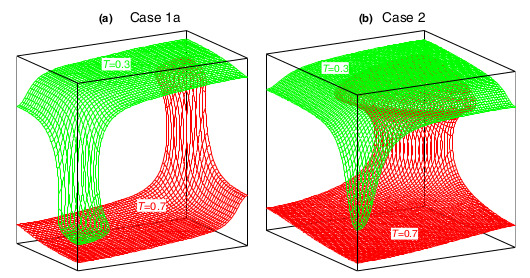
\includegraphics[height=4cm]{images/busse93/kaks05}
      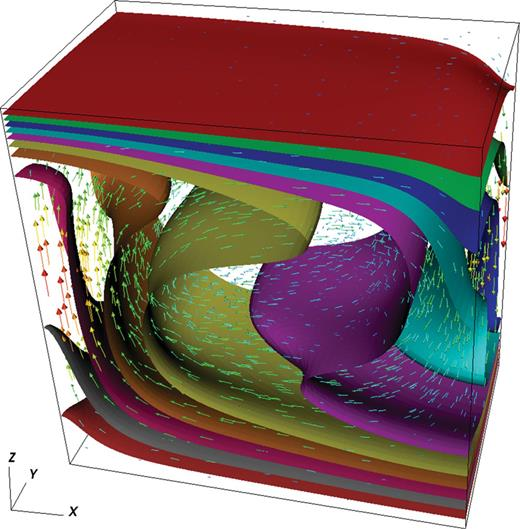
\includegraphics[height=4cm]{images/busse93/krhb12}\\
      {\captionfont Left: Taken from Kameyama \etal (2005).
      a) Isothermal surfaces obtained for the benchmark calculations 
      of stationary convections in Busse \etal. (1993). (a) Case 1a is for
      constant viscosity, while (b) Case 2 is for modestly temperature-dependent 
      viscosity whose viscosity contrast is 20. The calculations
      were carried out with (a) 64x32x64 and (b) 64x64x64 mesh divisions.
      Right: Taken from Kronbichler \etal (2012).}
      \end{center}

\item Numerical simulations of three-dimensional thermal convection in a fluid with strongly
      temperature-dependent viscosity: Ogawa \etal \cite{ogsz91,kaks05} 

\item Free surface evolution: Crameri \etal (2012) \cite{crsg12}, \aspect{} manual \cite{aspectmanual},
                              Schuh-Senlis \etal (2020) \cite{sctc20}
\item Love's problem: Becker \& Bevis (2004) \cite{bebe04}
\item Poiseuille flow: \cite{fojg94,fuku11,tagm09} (see Section~\ref{ss:poiseuille})
\item Couette flow with temperature dependent viscosity \cite{egat10,demh19}
\item Couette flow with shear heating \cite{egat10}
\item Poiseuille-Couette flow \cite{fusc13}
\item Lid driven cavity \cite{kawa61,chor67,shry78,foth79,ghgs82,kost84,bope98,xika01,brsa06,ertu09}
\item Lid driven cavity with analytical solution (see Section~\ref{sec:ldc_anal})
\item Lid driven cavity with nonlinear rheology \cite{been80,svna18}
\item Wannier flow \cite{wann50,yemu99,cehg14}
\item bending of elastic plate/beam \cite{cehg14,boht08a,vosc15,egat10,demh19,modm02,litu02}
\item flexure of finite length elastic plate \cite{chtl13}
\item thermal diffusion of half-cooling space (see Section~\ref{sec:hcsp}) 
\item thermal diffusion of Gaussian distribution (see compgeo notes, elefant manual)
\item stress build-up in Maxwell visco-elastic material \cite{geyu07,chtl13,egat10,demh19}
\item plastic oedometer test  \cite{chtl13}
\item channel flow (nonlinear) \cite{maie12,frbt19,gery10,egat10} (\bscthesis) \index{general}{BSc Thesis}
\item relaxation of sinusoidal interface \cite{crsg12,robh17}
\item single layer visco-elastic folding \cite{scps01,vosc15}
\item Three-dimensional folding of an embedded viscous layer in pure shear \cite{flet91}
\item dam-break problem \cite{moeb99,bacp07,liir07,lemx08,homa09,anco09,grdn97,hini81,basd08}
\item hot blob problem \cite{bugs09,fumt11} (see Section~\ref{sec:hotblob})
\item viscous(-elastic) flow around a cylinder in a channel (see Section~\ref{sec:flowcyl})
\item Sinking cylinder (2D Stokes sphere): appendix A of \cite{boht08a}, \cite{wali04}.
\item Infinite plate with a circular hole \cite{yiha10,rama16}
\item Semi-infinite elastic half plane with a circular hole \cite{verr98}
\item Slope stability for elasto-plastic materials \cite{rama16}
\item Time-dependent flow in an annulus \cite{galb19} (see Section \ref{sec:tdba})
\item Convection in 2D-box \cite{galb19} (see Section~\ref{sec:citb})
\item Onset of convection \cite{aspectmanual}
\item Polydiapirism \cite{wesc92,aspectmanual}
\item Slab detachment benchmark (see Section~\ref{sec:slabdetach}) 
\item 3D Hollow sphere Stokes flow benchmark:\\
      Thieulot (2017) \cite{thie17},
      Horbach \etal (2020) \cite{homb20}
\item Axisymmetric hollow sphere compressible Stokes flow benchmark:\\
      Machetel \& yuen (1989) \cite{mayu89}
\item Annulus benchmark \cite{aspectmanual}, \cite{ples11}

\item Viscosity grooves benchmark \cite{aspectmanual}
\item Latent heat benchmark \cite{aspectmanual}
\item Layered flow with viscosity contrast \cite{aspectmanual} (see Section \ref{sec:layfl}) 
\item Brittle thrust wedges benchmark \cite{busa16,aspectmanual}
\item mantle convection in 3D spherical shell:
      Ratcliff \etal \cite{rasz96},
      Iwase (1996) \cite{iwas96},
      Zhong \etal (2000) \cite{zhzm00},
      Yoshida \& Kageyama \cite{yoka04},
      Stemmer \etal (2006) \cite{sthh06},
      Choblet \etal (2007) \cite{chcc07},
      Zhong \etal (2008) \cite{zhmt08},
      Kameyama \etal (2008) \cite{kaks08},
      Wright \etal (2010) \cite{wrfy10},
      Davies \etal (2013) \cite{dadb13},
      Burstedde \etal (2013) \cite{busa13},
      Arrial \etal (2014) \cite{arfw14},
      Liu \& King (2019) \cite{liki19}
\item Heat flow around a cylinder (see Section~\ref{sec:hfcyl})
\item Laplace equation on a semi infinite plate (see Section~\ref{sec:lapplate})
\item 2D Stokes flow over cavity: Popov \& Makeev (2014) \cite{poma14}.
\item fractal networks of  shear bands: Poliakov \& Herrmann (1994) \cite{pohe94}
\item Square plate with a crack subjected to a horizontal tensile traction \cite{litu02}
\item Analytical solution for solitary porosity waves: Connolly \& Podlachikov (2015) \cite{copo15}
\item Analytical solution for solitary wave of magma: Dannberg \& Heister (2016) \cite{dahe16} and refs therein
\item Stokes flow caused by the motion of a rigid sphere close to a viscous interface: 
      Danov \etal (1998)  \cite{dagr98}
\item Deformation caused by a closed vertical volcanic pipe \cite{boda99}
\item Mantle convection with reversing mobile plates \cite{kogk05}
\item A comparison of mantle convection models featuring plates \cite{stlh14}
\item Elastic material in simple shear (see Section~\ref{sec:elastsimpshear})
\item Elastic material in pure shear (see Section~\ref{sec:elastpureshear})
\item Hole in an Elastic material with a circular hole (see Section~\ref{sec:elastic_hole})
\item Uniform strip load on elastic material (see Section~\ref{sec:elaststripload})
\item Linear Stability Analysis for Thermal Convections in Spherical Shells \cite{yuwa19}
\item Channel flow: Mancktelow (2008) \cite{manc08}
\item Viscous half-space loading \cite{hask35}
\item Nakiboglu and Lambeck (1982) has cylindrical load on variety of rheologies \cite{nala82}
\item Jull and McKenzie (1996) \cite{jumc96} parabolic load on viscoelastic half-space (and melt fractions) 
\item Squeezing flow between moving parallel plates \cite{gugu77}
\item generalized half-plane and half-space Cerruti \cite{nowi92,zhga15}
\item Analytical Solutions of Displacements Produced by spherically-shaped Internal Overpressure \cite{gech12}
\item Sagging viscous bridge \cite{stokes98}
\item Deformation around a terminating fault in a viscous medium \cite{baho96}
\end{itemize}


%.......................................................
\subsubsection{Poiseuille flow} \label{ss:poiseuille}

We consider a two-dimensional channel in the $x,y$ plane. The walls 
are at $y=0$ and $y=H$ with no-slip boundary conditions. 
In the absence of gravity, the Stokes equation simplify to 
\begin{equation}
-\frac{\partial p}{\partial x}  +\frac{\partial }{\partial y} (2\eta_0 \dot{\varepsilon}_{xy}) =0
\qquad
\text{and}
\qquad
\dot{\varepsilon}_{xy} = \frac{1}{2} \frac{\partial u}{\partial y} 
\label{eq:pois1}
\end{equation}
where we assume the velocity $\vec\upnu=(u(y),0)$.
In the case of a Newtonian fluid, the analytical solution is 
known and the velocity profile is a parabola with zero velocity on the
walls and maximum velocity in the middle. 


Eq.~\eqref{eq:pois1} must then be solved 
\begin{eqnarray}
\frac{\partial p}{\partial x}  
&=&\frac{\partial }{\partial y} \left(2\eta_{0}  \frac{1}{2}\frac{\partial u}{\partial y} \right) 
= \eta_0 \frac{\partial^2 u}{\partial y^2}  
\end{eqnarray}

We pose $\Pi=\frac{\partial p}{\partial x}<0$, i.e. 
there is more pressure applied to the left than to the right of the channel.
We then must solve:
\[
\frac{\partial^2 u}{\partial y^2} = \frac{\Pi}{\eta_0} 
\]
The solution is then of the form
\[
u(y) = \frac{1}{2}\frac{\Pi}{\eta_0} y^2 + 2a y + b
\]
and 
\[
\dot{\varepsilon}_{xy}= \frac{1}{2} \frac{\Pi}{\eta_0}y  + a
\]
We will now determine $a$ and $b$.

The velocity must be zero at $y=0$ and $y=H$ so 
\[
u(y=0)=b=0
\] 
and 
\[
u(y=H)=\frac{1}{2}\frac{\Pi}{\eta_0} H^2 + 2a H =0
\]
or, 
\[
2a=-\frac{1}{2}\frac{\Pi}{\eta_0} H
\]
so 
\begin{equation}
\boxed{
u(y) = \frac{1}{2}\frac{\Pi}{\eta_0} (y^2 - y H)
}
\end{equation}
and 
\begin{equation}
\boxed{
\dot{\varepsilon}_{xy}= \frac{1}{2} \frac{\Pi}{\eta_0} \left(y  - \frac{H}{2} \right)
}
\end{equation}
 


 











%..................................................
\subsubsection{Relaxation of sinusoidal topography}

Following Kramer \etal \cite[Section 3.1.1]{krwd12} and \cite{robh17} 
the benchmark consists of the relaxation of surface topography in a 
two-dimensional Cartesian box with an isoviscous fluid. 
Free slip boundary conditions are imposed on the sides and bottom of the domain.
The setup is as follows:

\begin{center}
\begin{minipage}{0.45\textwidth}
\centering
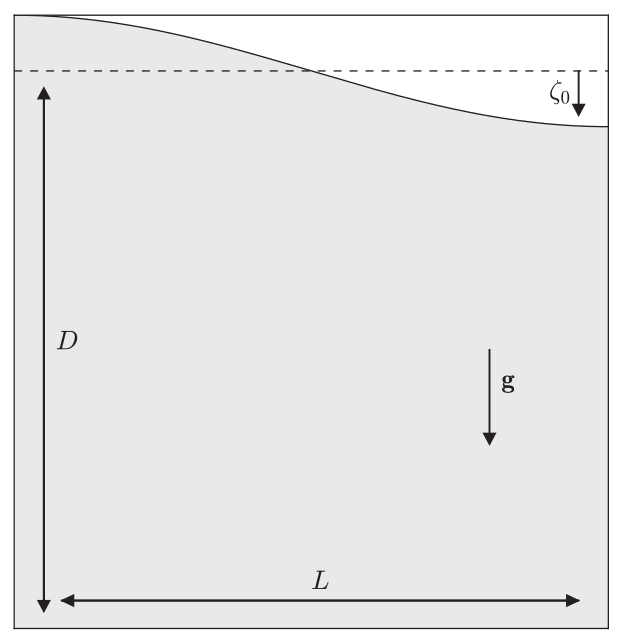
\includegraphics[height=0.8\textwidth]{images/benchmark_relaxation/robh17}\\
{\captionfont Taken from \cite{robh17}. Setup for the free surface relaxation benchmark.
For the tests $\rho=\eta=g=L=D=1$ and $\xi_0=0.005$.}
\end{minipage}\hfill
\begin{minipage}{0.45\textwidth}
\centering
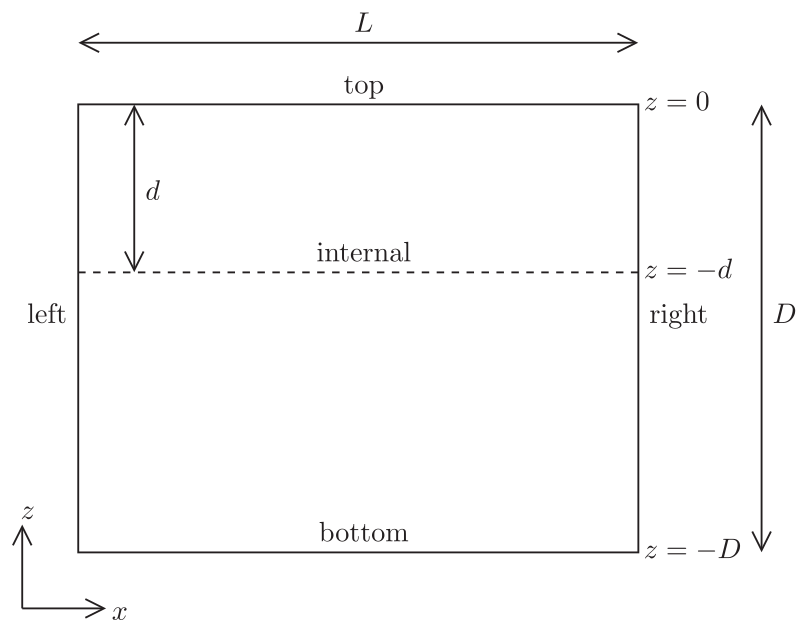
\includegraphics[height=0.8\textwidth]{images/benchmark_relaxation/krwd12}\\
{\captionfont Taken from \cite{krwd12}. $D=3\cdot 10^6$,$\eta=10^{21}$, $\rho=4500$, $g=10$, $\xi_0=10^3$m, and 
$L=D/4,D/2,D,2D,4D$.}
\end{minipage}
\end{center}
and the infinitesimal sinusoidal perturbations to the free surface is given by
\[
\xi(x,t=0)=\xi_0 \cos \left( \frac{2 \pi n x}{L}  \right)
\]
where $n$ is a wavenumber which is an integer multiple of 1/2 (taken to be 1/2 exactly in both cases).


%...............................................................
\subsubsection{the plastic brick} \label{ss:plasticbrick}

\Literature \cite{hans03,moml07,lemm08,kaus10,egat10,qurj09,mishin11,maie12,spmw16,gltf18,frbt19,aspectmanual}

Pretty much all of the brick-type (elasto-)visco-plastic experiments in the literature
introduce a weak seed at the bottom of the domain to seed deformation (the shear bands
will ultimately stem from it). 
Dimensioned and dimensionless experiments have been carried out, with or without 
elastic behaviour, with or without adaptive mesh refinement, with first order and 
second order quadrilateral elements or Taylor-Hood triangles, with or without 
Newton algorithm, in extension and compression, with or without time-stepping,
with or without viscous lower layer. 


\begin{center}
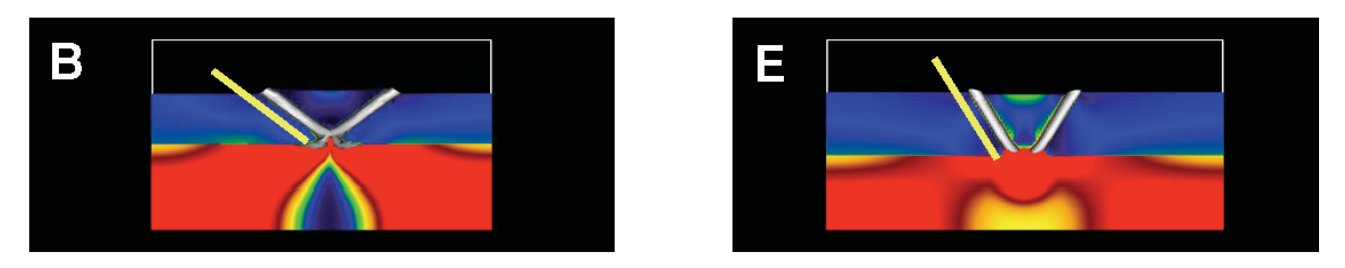
\includegraphics[width=7cm]{images/benchmark_brick/momu06}\\
{\captionfont Moresi \& M{\"u}lhaus, 2006 \cite{momu06}}
\end{center}

\begin{center}\noindent\rule{12cm}{0.4pt}\end{center}

\begin{center}
\begin{minipage}{0.45\textwidth}
\centering
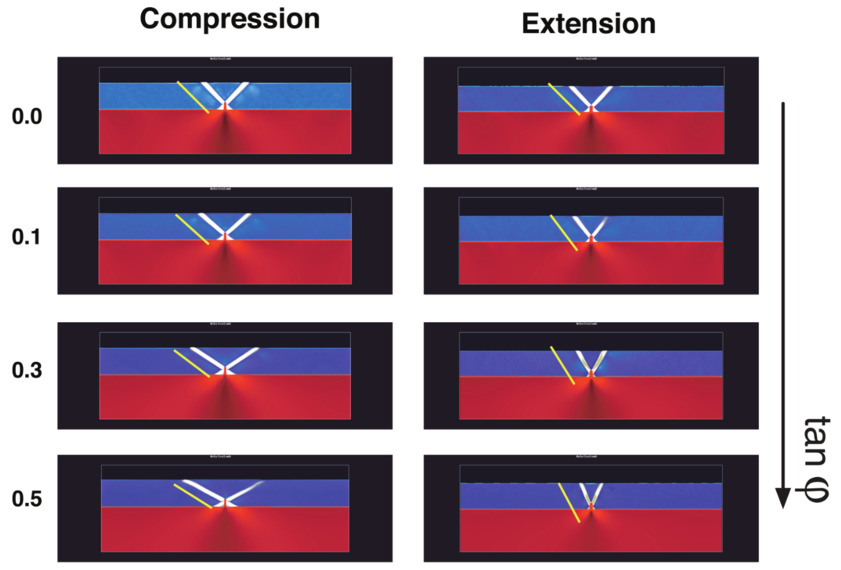
\includegraphics[height=0.8\textwidth]{images/benchmark_brick/moml07}\\
{\captionfont Moresi \etal, 2007 \cite{moml07}}
\end{minipage}\hfill
\begin{minipage}{0.45\textwidth}
\centering
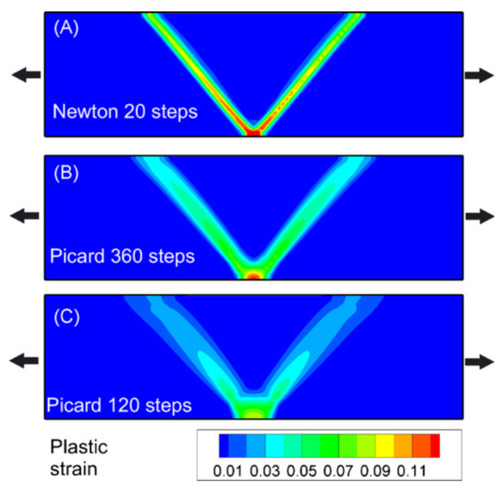
\includegraphics[height=0.8\textwidth]{images/benchmark_brick/poso08}\\
{\captionfont Popov \etal, 2008 \cite{poso08}}
\end{minipage}
\end{center}

\begin{center}\noindent\rule{12cm}{0.4pt}\end{center}

\begin{center}
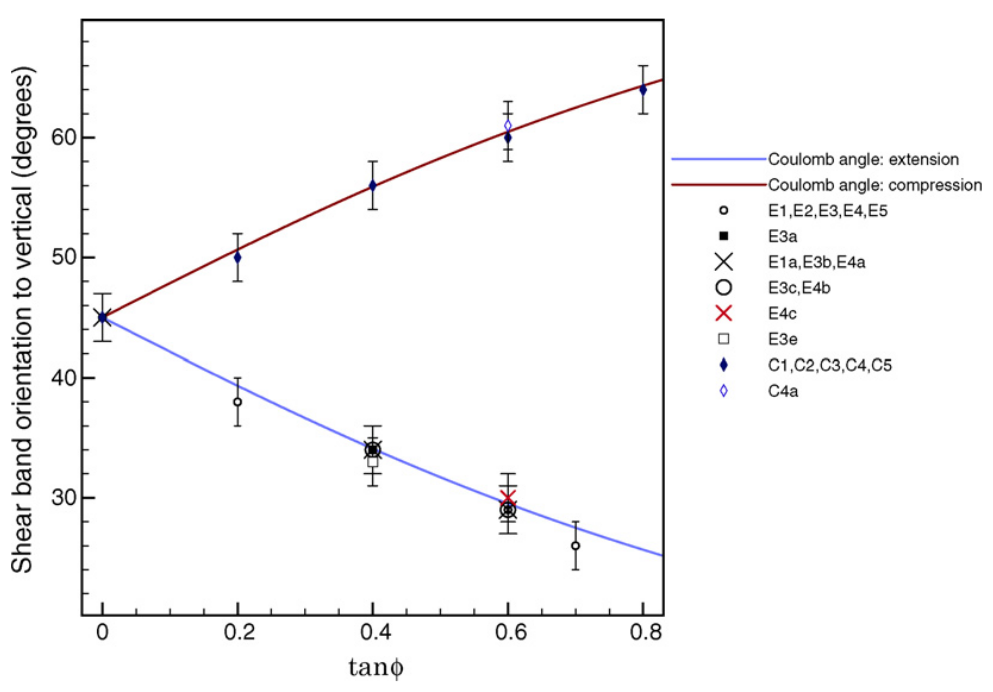
\includegraphics[width=5cm]{images/benchmark_brick/lemm08a}
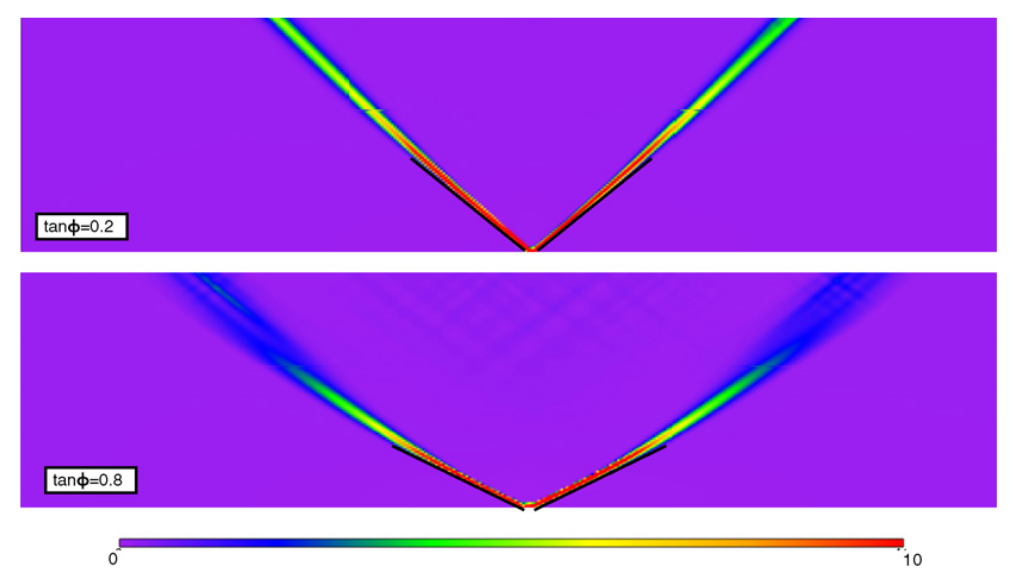
\includegraphics[width=5cm]{images/benchmark_brick/lemm08b}
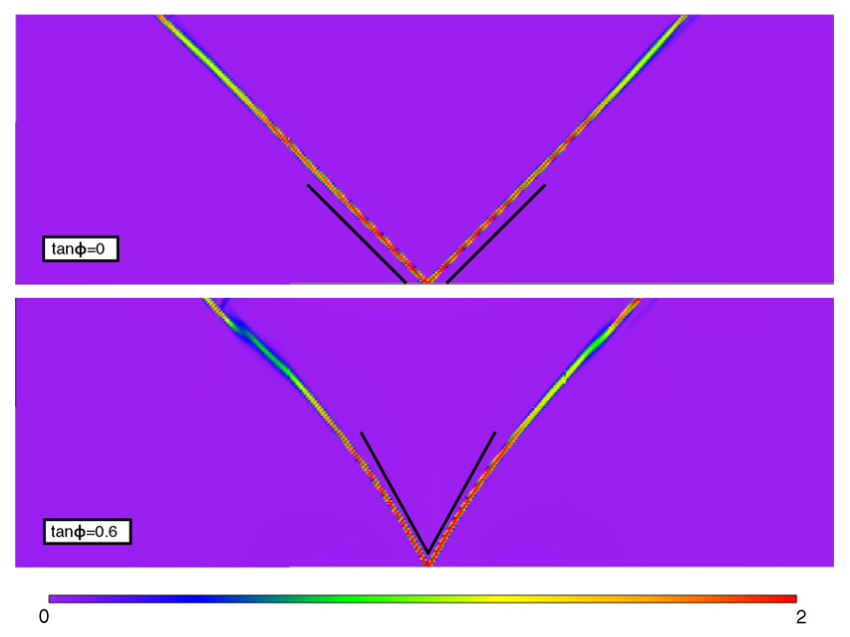
\includegraphics[width=5cm]{images/benchmark_brick/lemm08c}\\
{\captionfont Lemiale \etal, 2008 \cite{lemm08}}
\end{center}

\begin{center}\noindent\rule{12cm}{0.4pt}\end{center}

\begin{center}
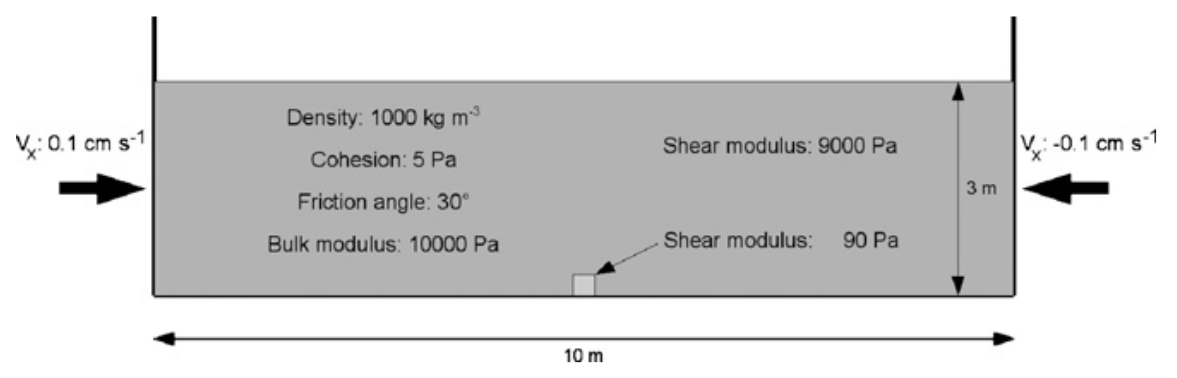
\includegraphics[width=7cm]{images/benchmark_brick/qurj09b}
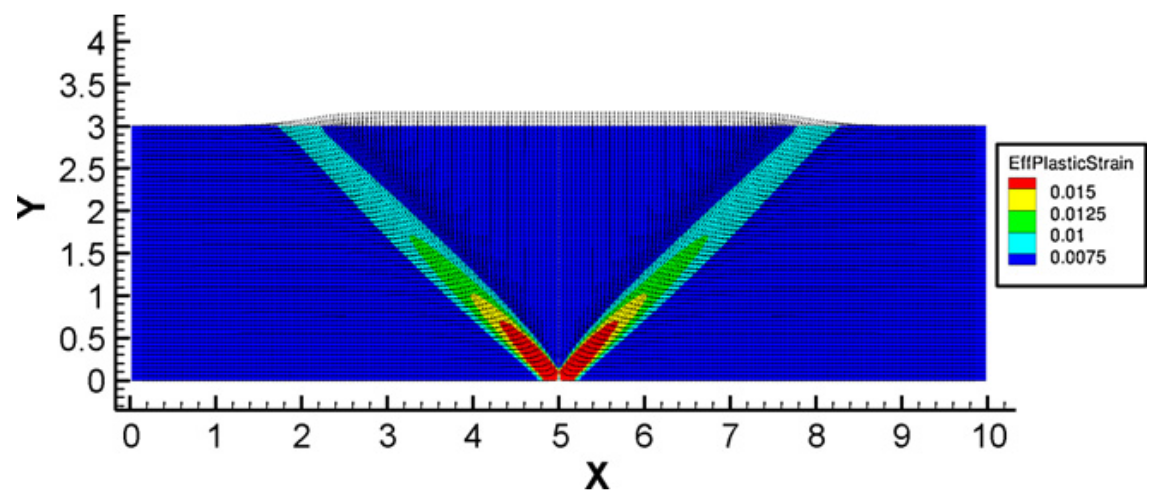
\includegraphics[width=6cm]{images/benchmark_brick/qurj09a}\\
{\captionfont Quinteros \etal, 2009 \cite{qurj09}}
\end{center}

\begin{center}\noindent\rule{12cm}{0.4pt}\end{center}

\begin{center}
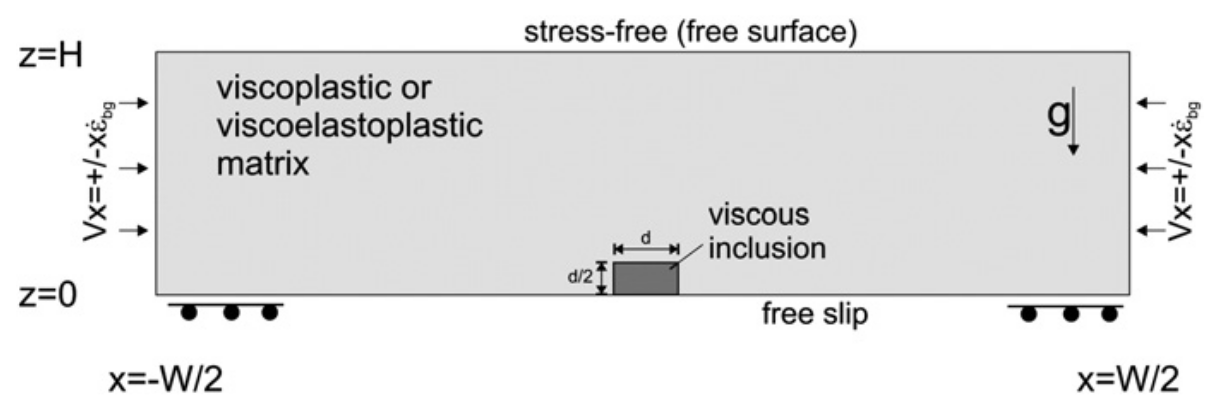
\includegraphics[width=5cm]{images/benchmark_brick/kaus10a}
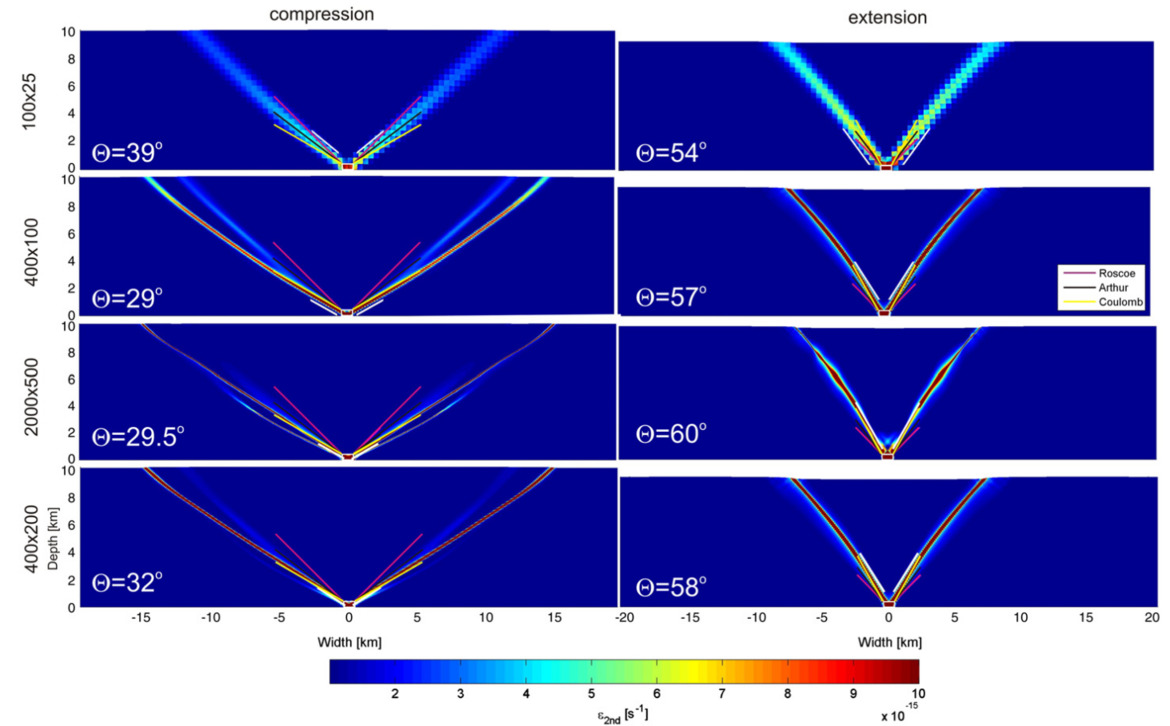
\includegraphics[width=5cm]{images/benchmark_brick/kaus10b}
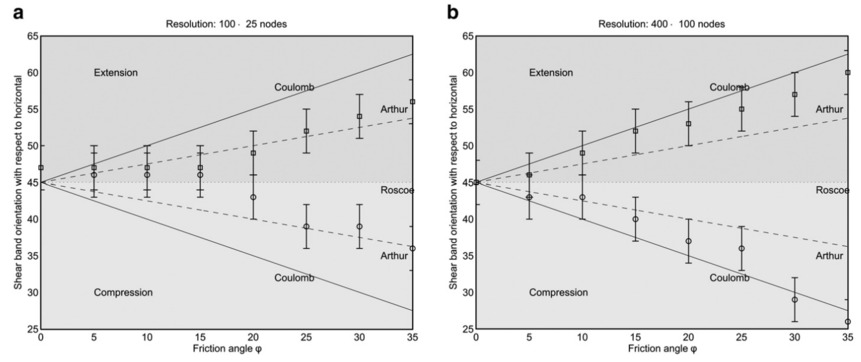
\includegraphics[width=5cm]{images/benchmark_brick/kaus10c}\\
{\captionfont Kaus, 2010 \cite{kaus10}}
\end{center}

\begin{center}\noindent\rule{12cm}{0.4pt}\end{center}

\begin{center}
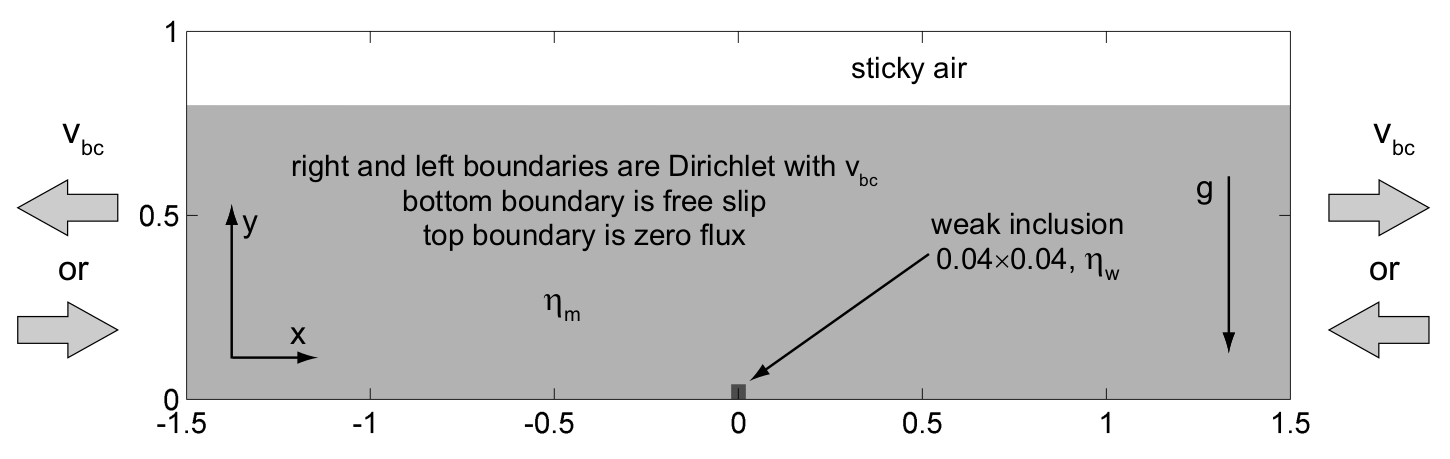
\includegraphics[width=3.74cm]{images/benchmark_brick/mishina}
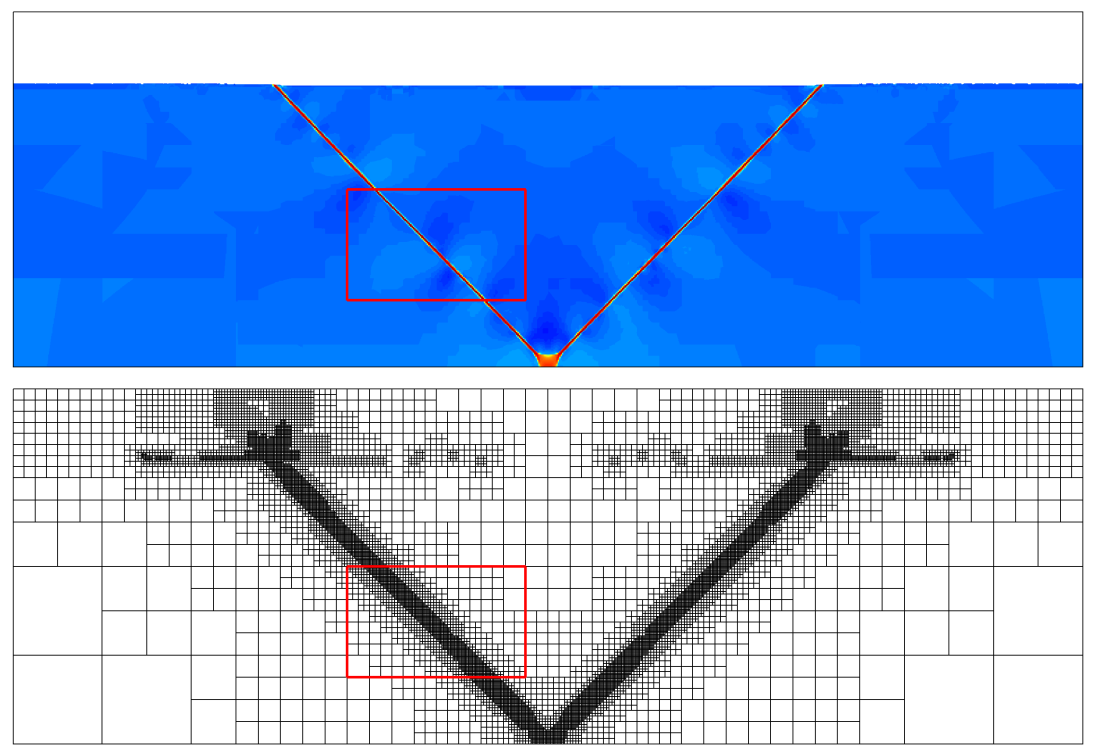
\includegraphics[width=3.74cm]{images/benchmark_brick/mishinb}
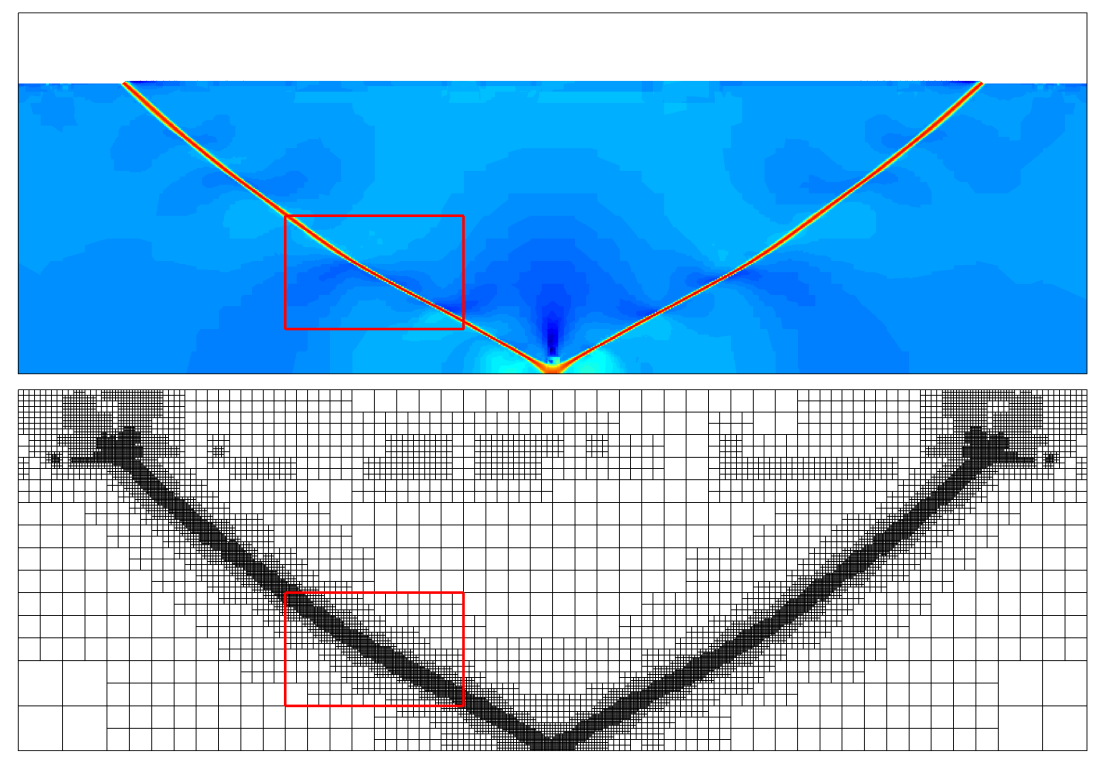
\includegraphics[width=3.74cm]{images/benchmark_brick/mishinc}
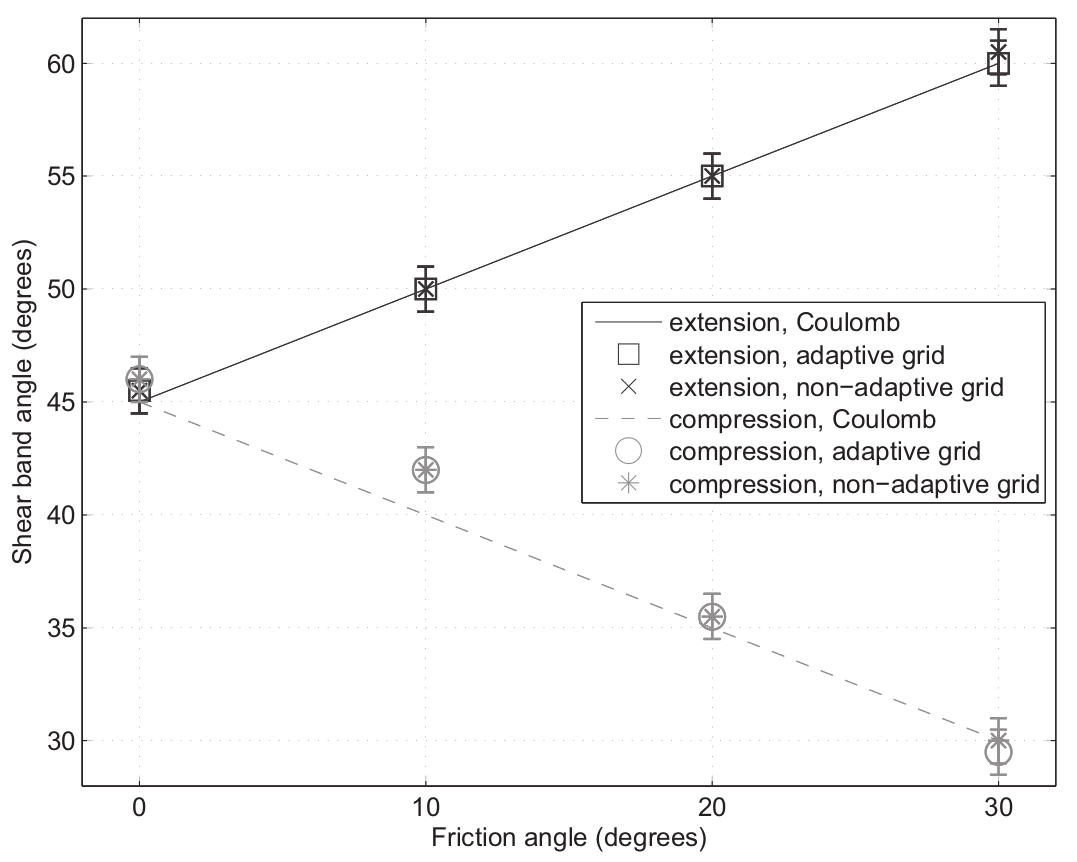
\includegraphics[width=3.74cm]{images/benchmark_brick/mishind}\\
{\captionfont Mishin, phd thesis, 2011 \cite{mishin11}}
\end{center}

\begin{center}\noindent\rule{12cm}{0.4pt}\end{center}

\begin{center}
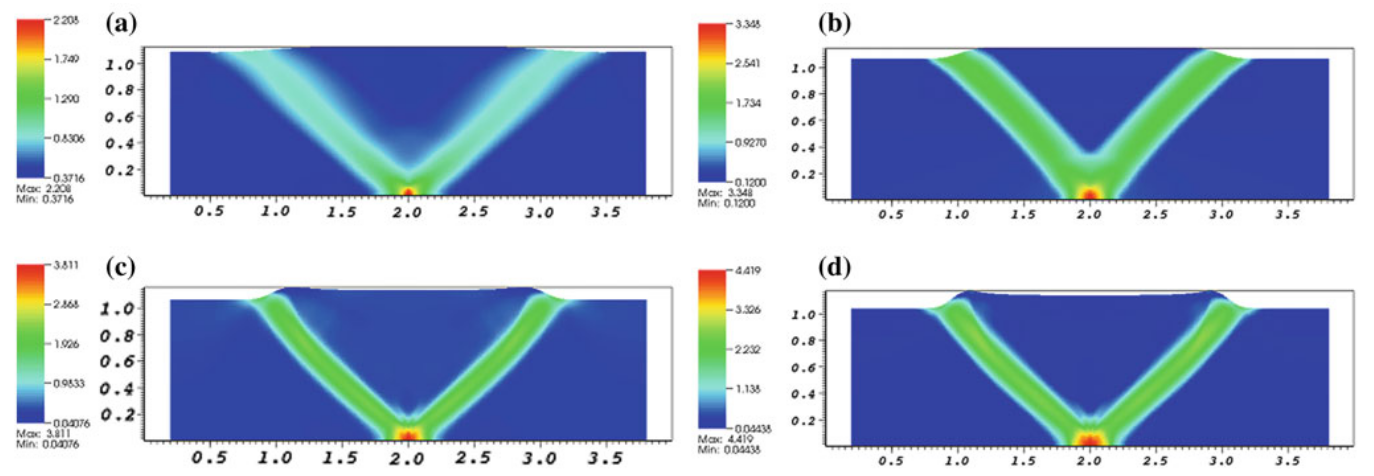
\includegraphics[width=9cm]{images/benchmark_brick/muso11}\\
{\captionfont M{\"u}hlhaus \etal, 2011 \cite{muso11}.}
\end{center}

\begin{center}\noindent\rule{12cm}{0.4pt}\end{center}

\begin{center}
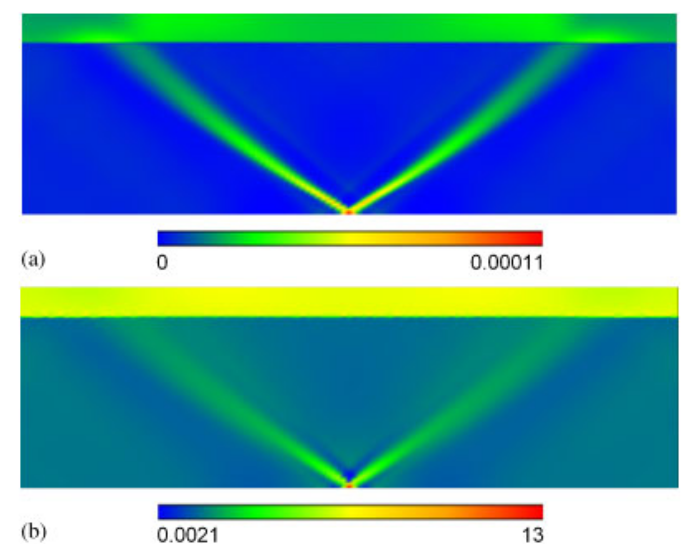
\includegraphics[width=9cm]{images/benchmark_brick/lemm11}\\
{\captionfont Lemiale \etal, 2011 \cite{lemm11}.}
\end{center}

\begin{center}\noindent\rule{12cm}{0.4pt}\end{center}

\begin{center}
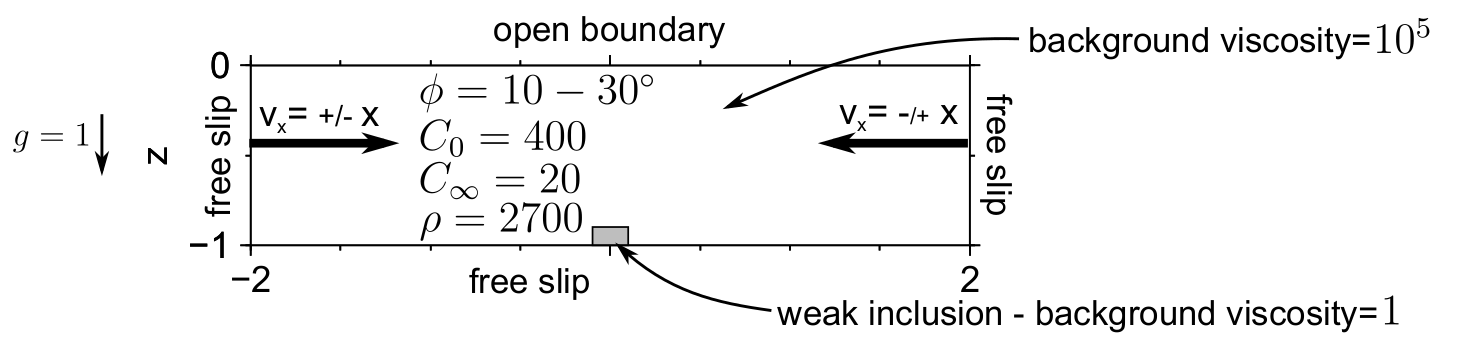
\includegraphics[width=8cm]{images/benchmark_brick/maie12a}
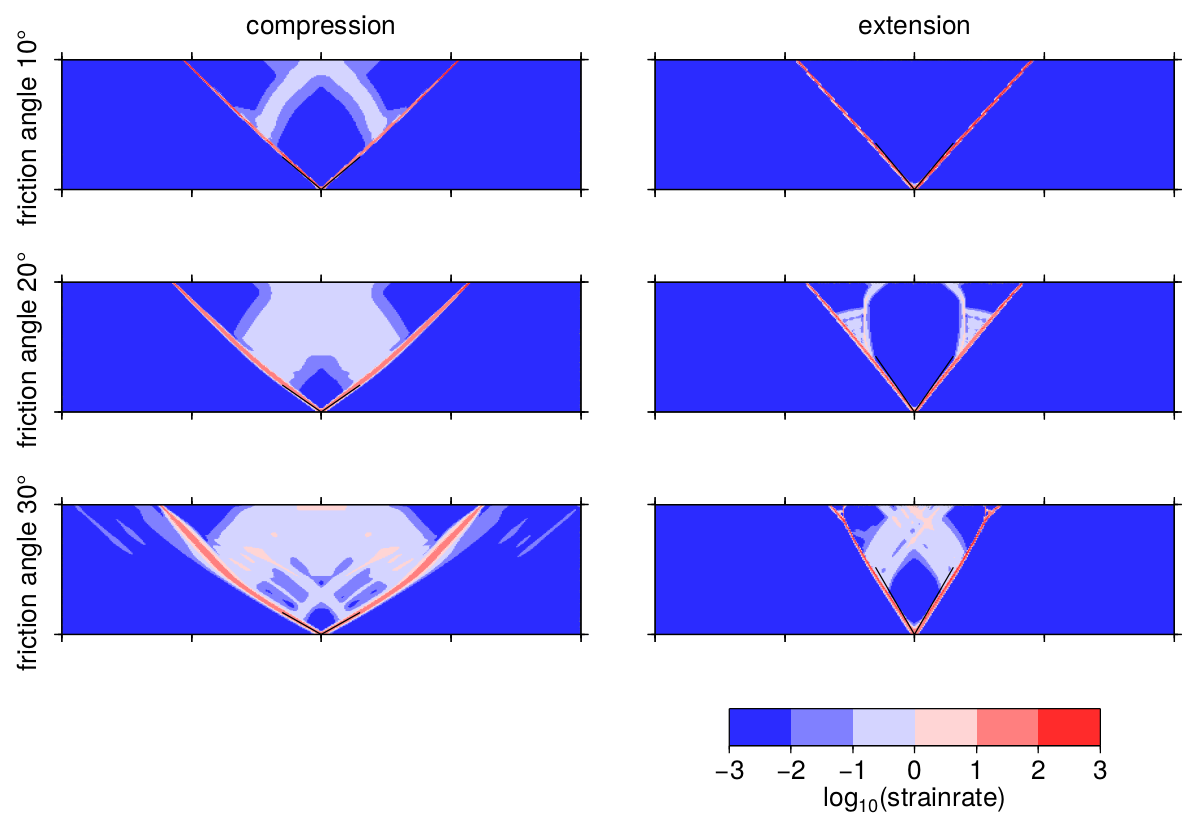
\includegraphics[width=5cm]{images/benchmark_brick/maie12b}\\
{\captionfont Maierova, phd thesis, 2012 \cite{maie12}}
\end{center}

\begin{center}\noindent\rule{12cm}{0.4pt}\end{center}

\begin{center}
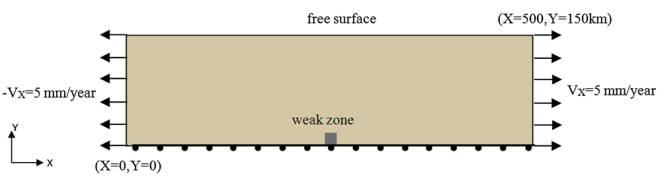
\includegraphics[width=5cm]{images/benchmark_brick/mofm13a}
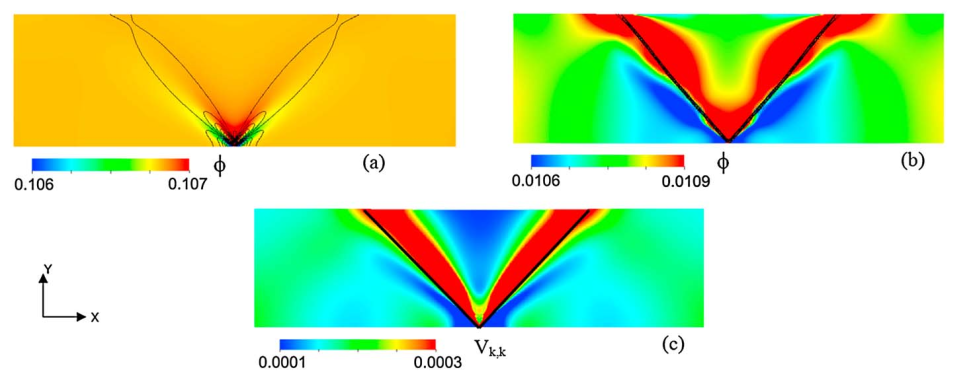
\includegraphics[width=8cm]{images/benchmark_brick/mofm13b}\\
{\captionfont Mohajeri \etal, 2013 \cite{mofm13}.}
\end{center}

\begin{center}\noindent\rule{12cm}{0.4pt}\end{center}

\begin{center}
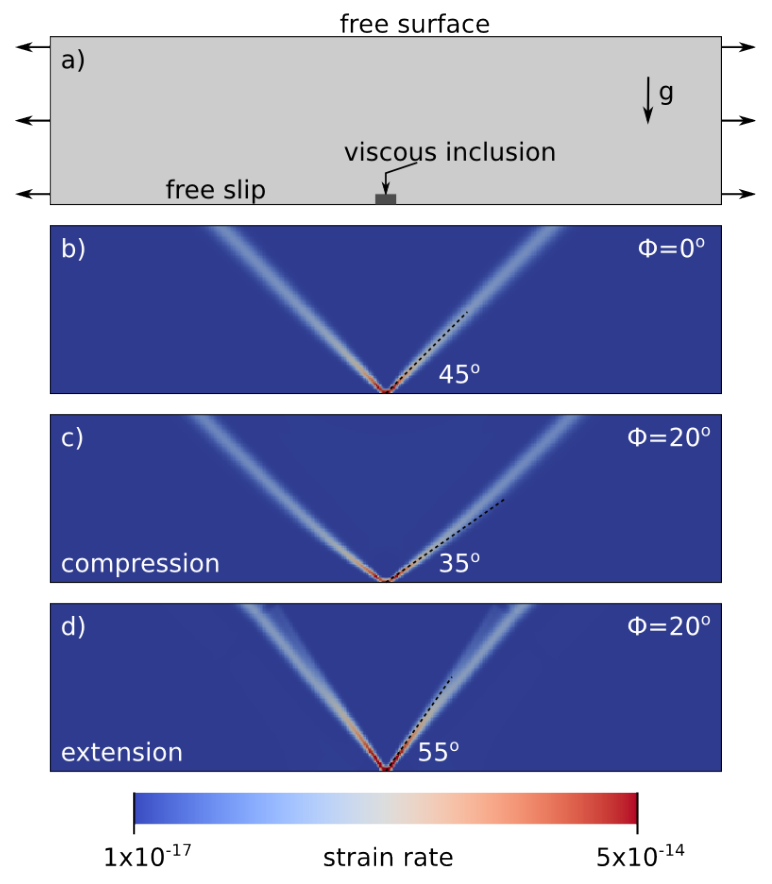
\includegraphics[width=5cm]{images/benchmark_brick/thie14a}
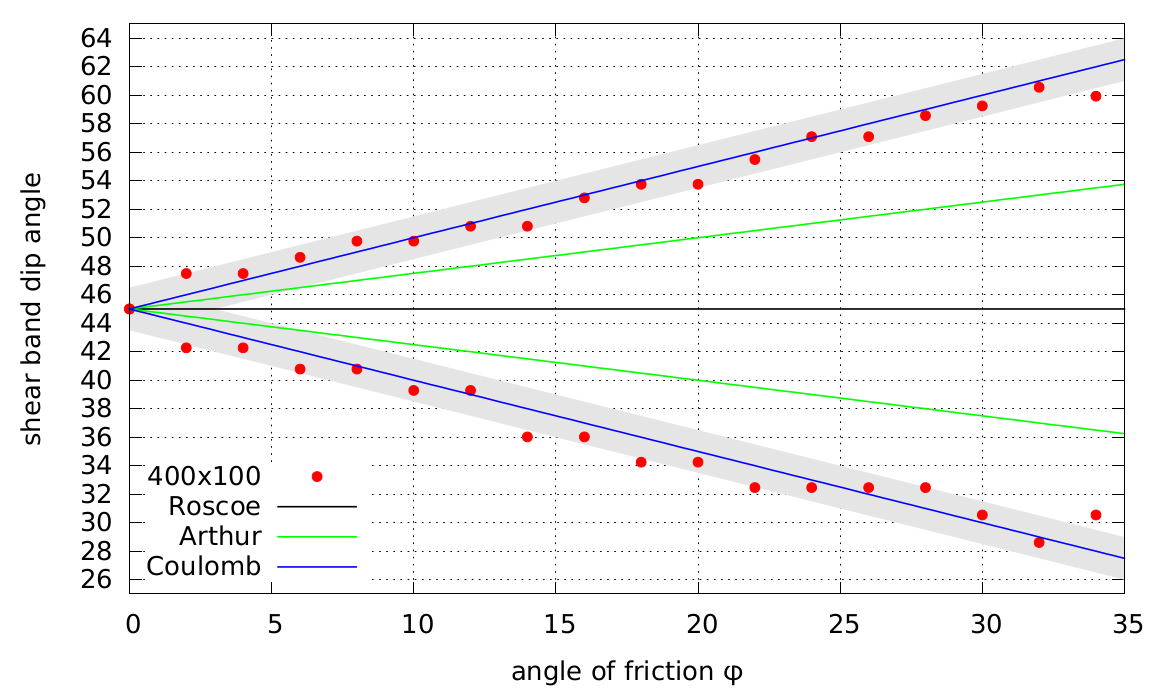
\includegraphics[width=8cm]{images/benchmark_brick/thie14b}\\
{\captionfont Thieulot, 2014 \cite{thie14}.}
\end{center}

\begin{center}\noindent\rule{12cm}{0.4pt}\end{center}

\begin{center}
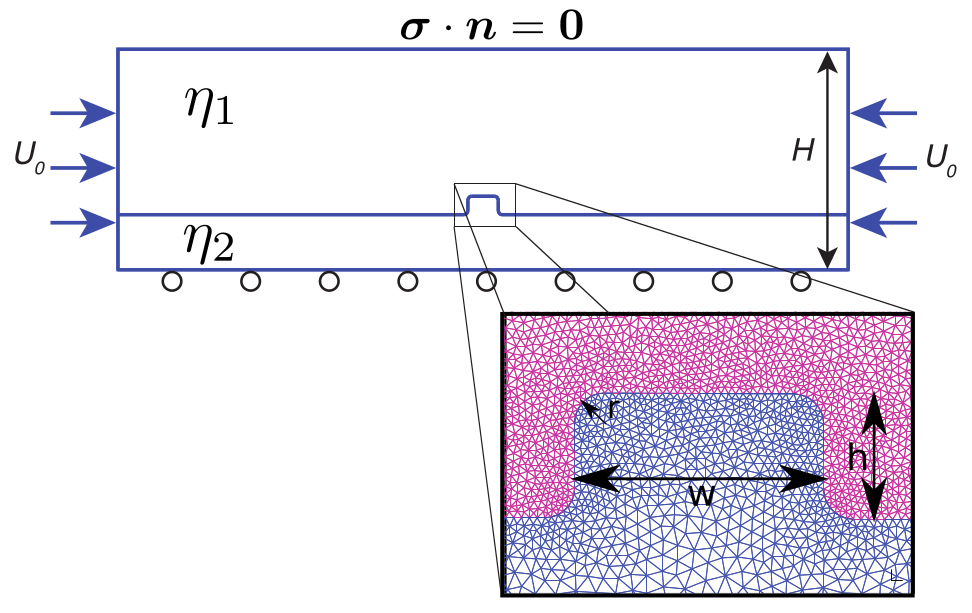
\includegraphics[width=5cm]{images/benchmark_brick/spmw16a}
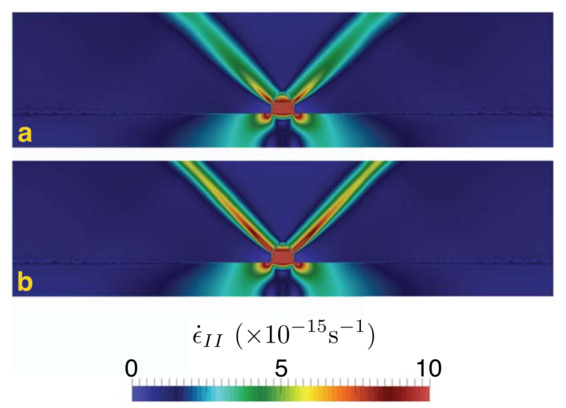
\includegraphics[width=5cm]{images/benchmark_brick/spmw16b}\\
{\captionfont Spiegelman \etal, 2016 \cite{spmw16}}
\end{center}

\begin{center}\noindent\rule{12cm}{0.4pt}\end{center}

\begin{center}
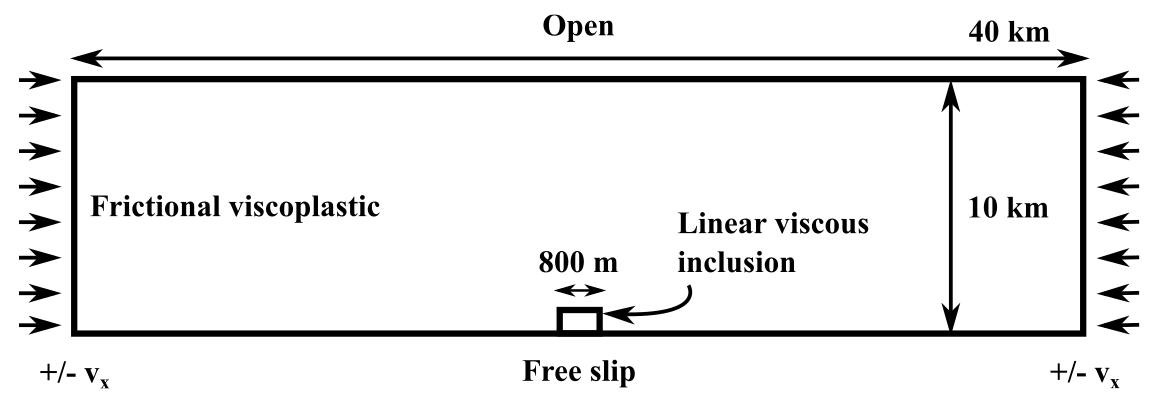
\includegraphics[width=5cm]{images/benchmark_brick/gltf18a}
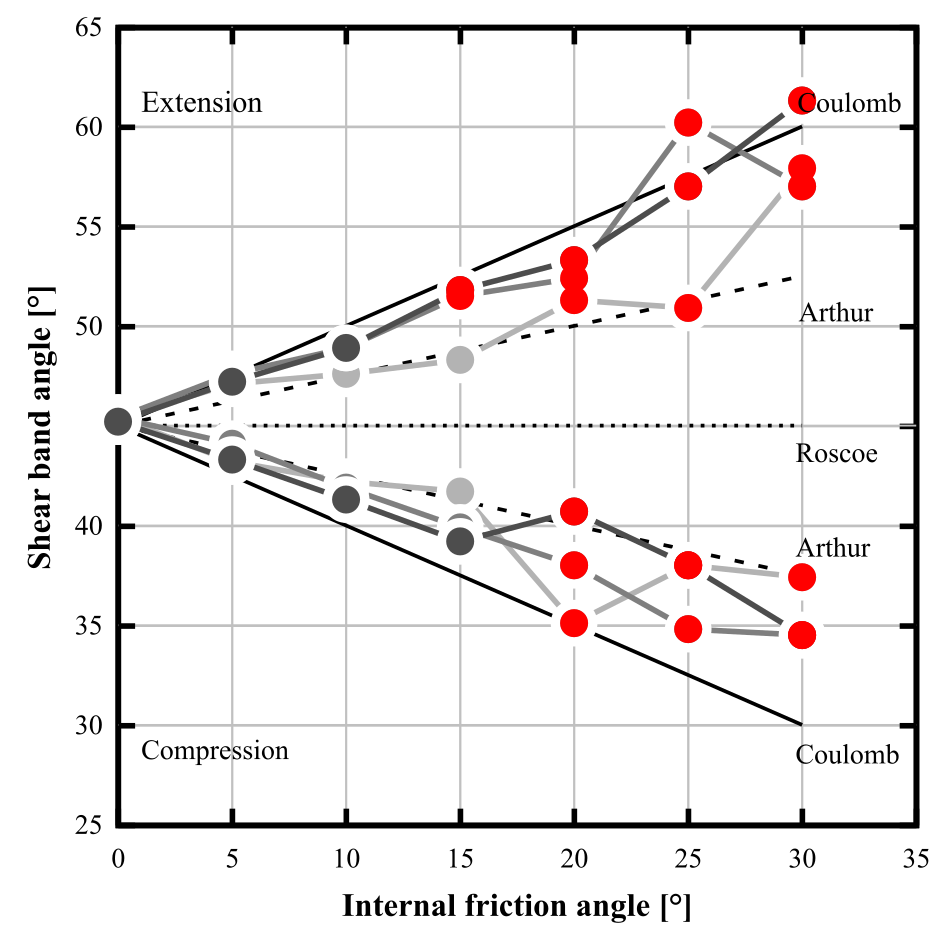
\includegraphics[width=5cm]{images/benchmark_brick/gltf18b}
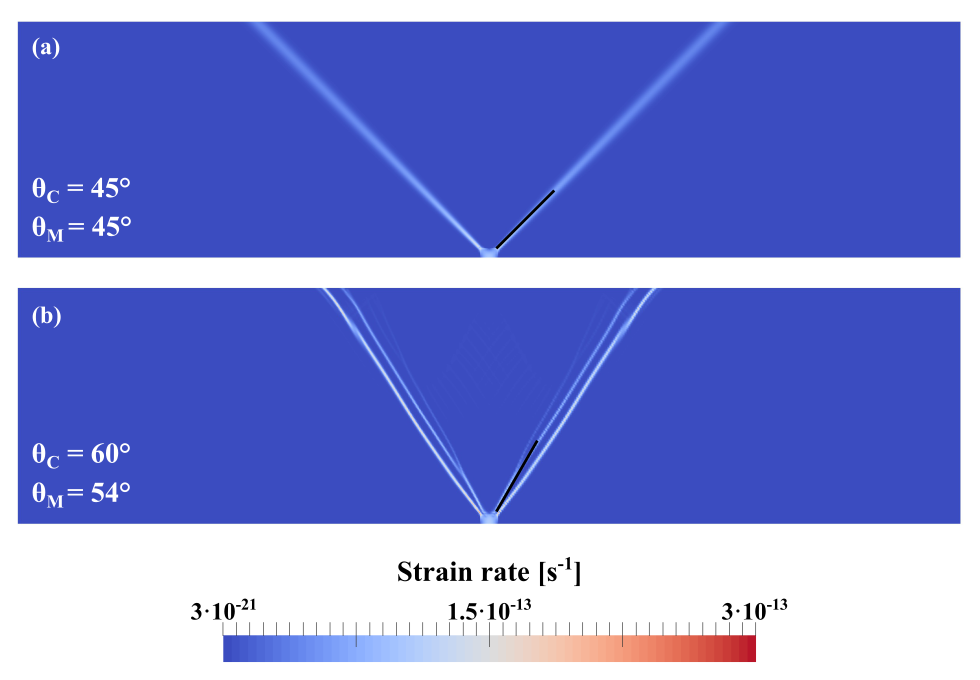
\includegraphics[width=5cm]{images/benchmark_brick/gltf18c}\\
{\captionfont Glerum \etal, 2018 \cite{gltf18}}
\end{center}

\begin{center}\noindent\rule{12cm}{0.4pt}\end{center}

\begin{center}
\begin{minipage}{0.45\textwidth}
\centering
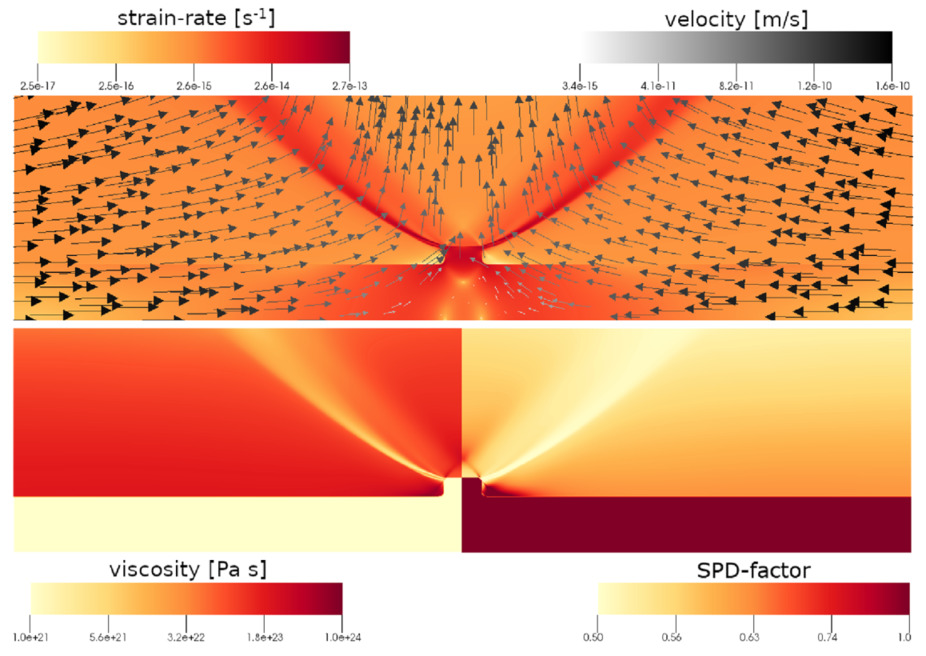
\includegraphics[height=0.8\textwidth]{images/benchmark_brick/frbt19}\\
{\captionfont Fraters \etal, 2019 \cite{frbt19}}
\end{minipage}\hfill
\begin{minipage}{0.45\textwidth}
\centering
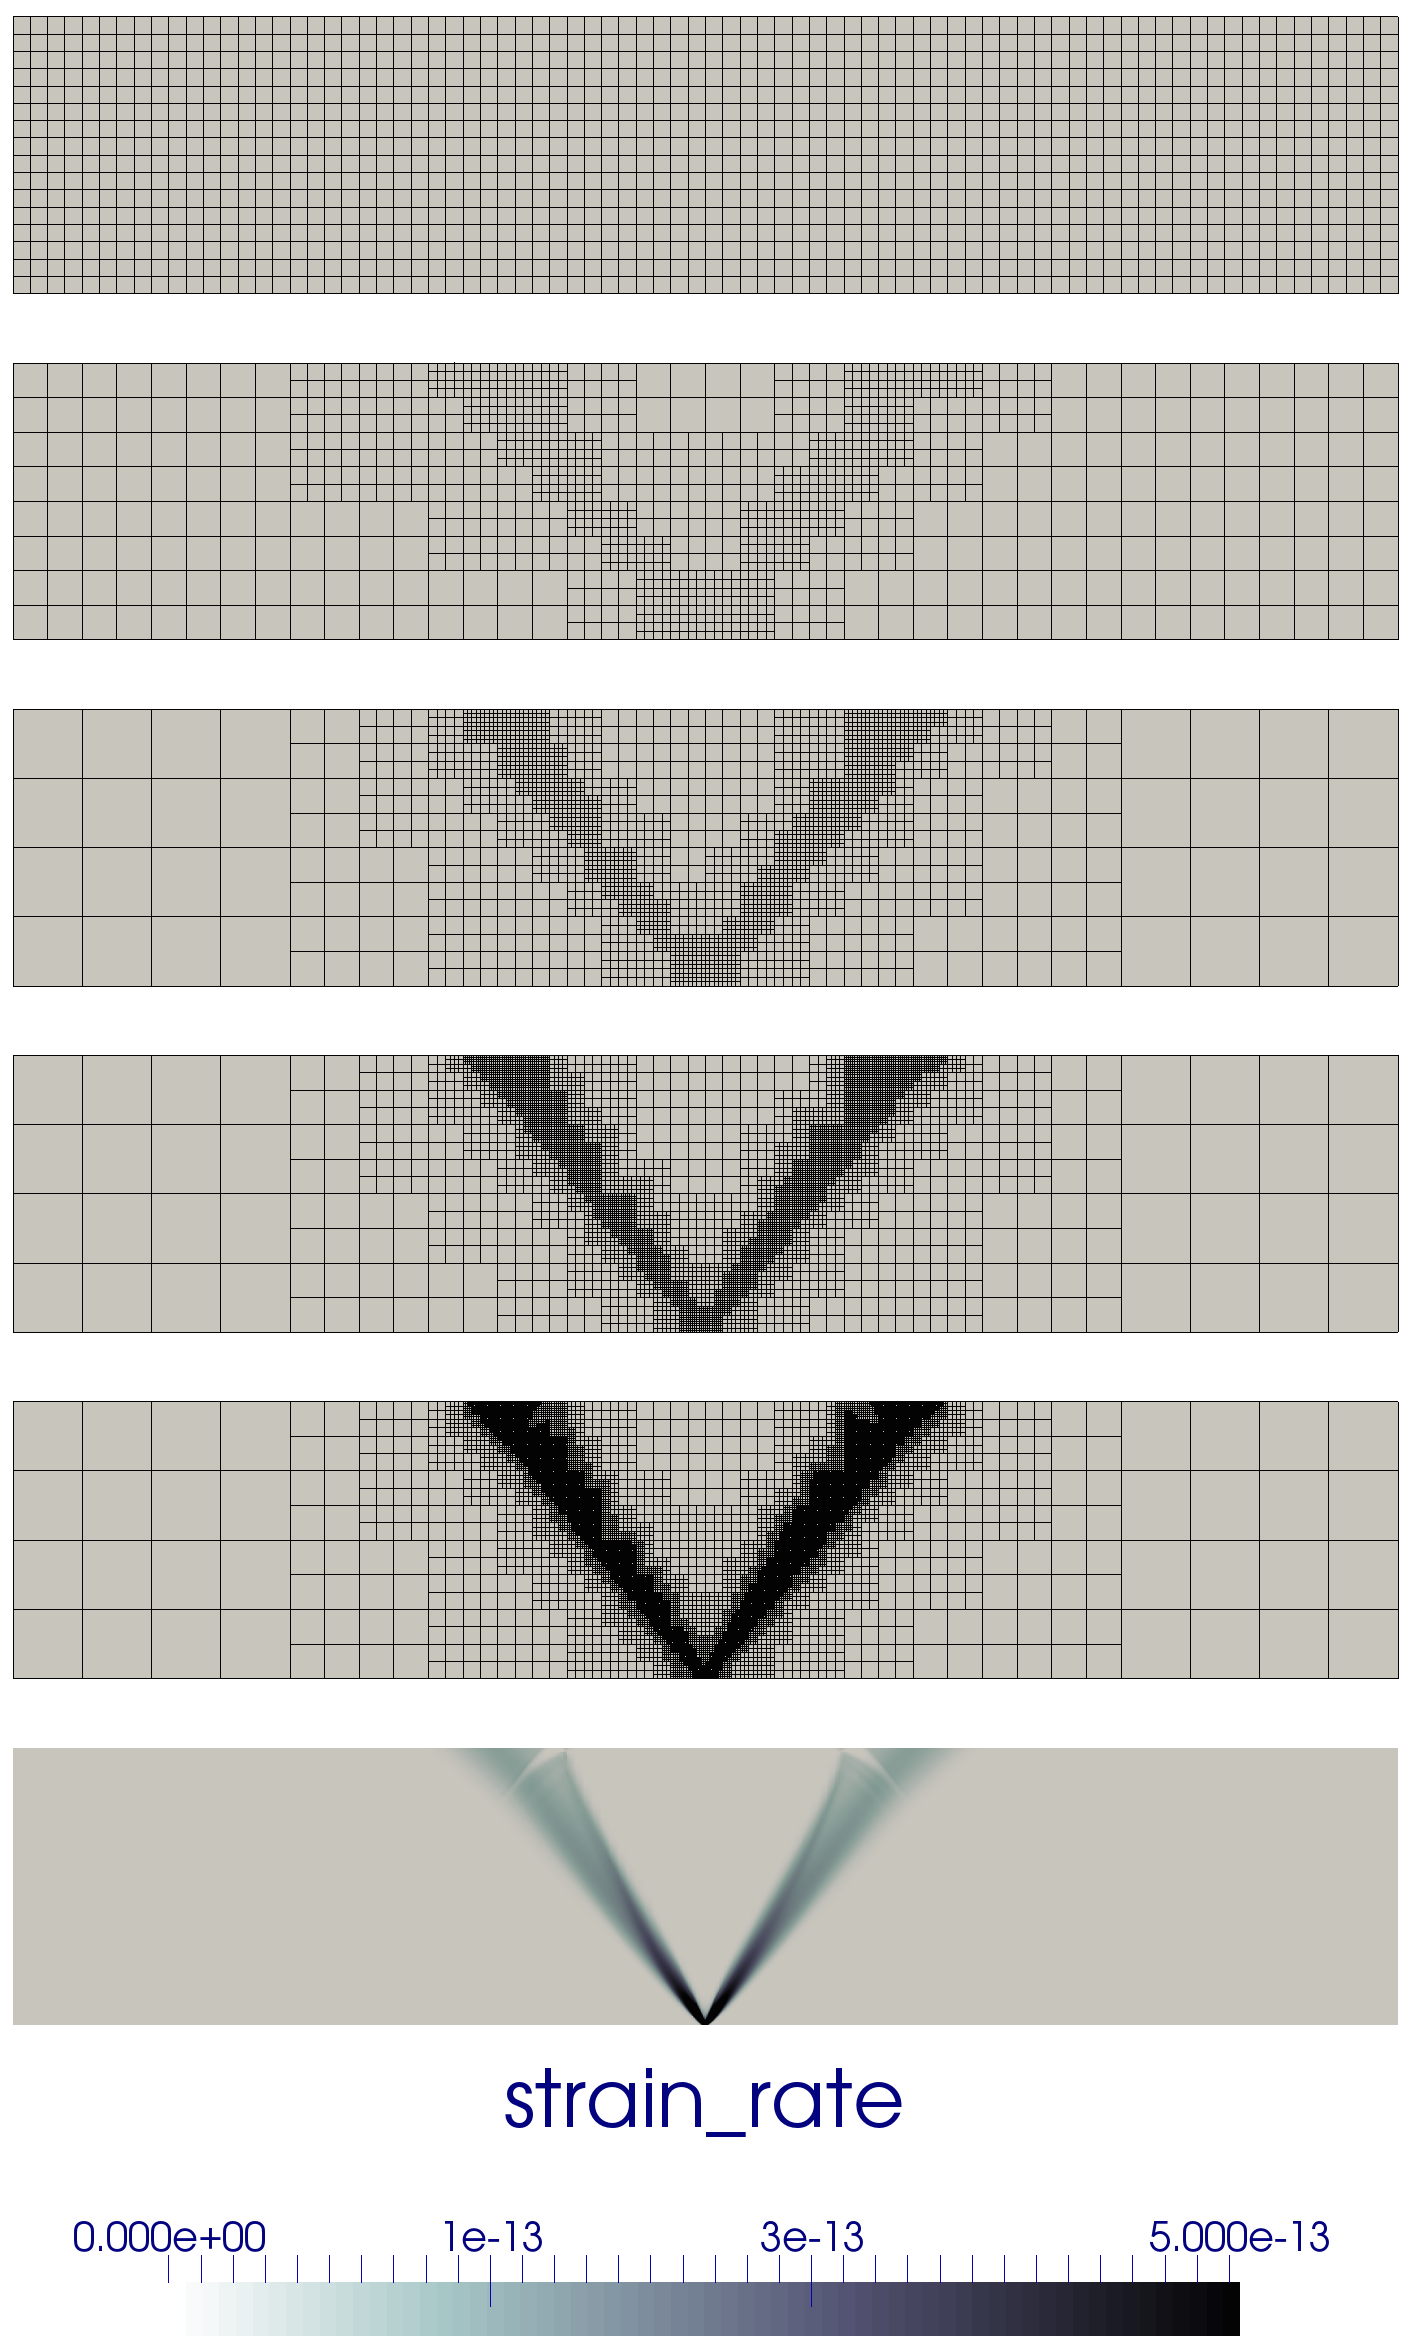
\includegraphics[height=0.8\textwidth]{images/benchmark_brick/aspectmanual}\\
{\captionfont Aspect manual \cite{aspectmanual}}
\end{minipage}
\end{center}

%..........................................................................
\subsubsection{Infinite plate with a circular hole \cite{rama16}}
\mscthesis \index{general}{MSc Thesis}

An infinite plate with a circular hole of radius $a$ 
is subjected to a unidirectional tensile load of $\sigma$ in the $x$ direction as shown
in the figure. In this case, only one quarter of the domain is analysed due
to symmetry along $x$ and $y$ axis. 

\begin{center}
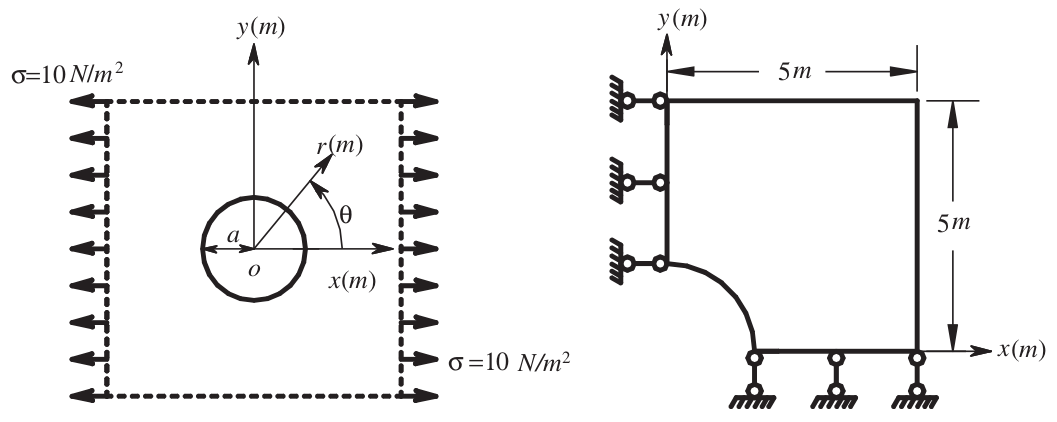
\includegraphics[width=0.65\textwidth]{images/benchmark_hole/yobu02}
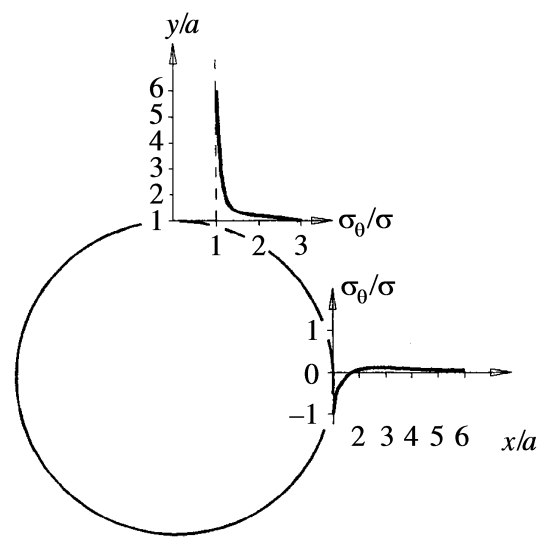
\includegraphics[width=0.25\textwidth]{images/benchmark_hole/yobu02b}\\
{\captionfont Left: An infinite plate with a circular hole subjected to unidirectional tension 
and its quarter model with symmetric conditions imposed on the left and bottom edges.
Right: Tangential stress distribution for $\theta=0$  and $\theta=\pi/2$. \cite{yobu02}}
\end{center}

The inner boundary of the hole is traction free and the right edge was
imposed with the tractions based on the analytical solutions.
The left edge is constrained in the $x$ direction and the bottom
edge is constrained in the $y$ direction, respectively. The plane stress
condition is considered and the parameters are: 
Young modulus $E=$3e7 MPa, Poisson Ratio $\nu=$0.3, Load $\sigma$=10 N/m$^2$, a=1m.

The analytical stress components for this
problem are 

\begin{eqnarray}
\sigma_{xx}(x,y) &=& \sigma \left(  1-\frac{a^2}{r^2}\left(\frac{3}{2}\cos 2\theta + \cos 4\theta \right) 
+ \frac{3a^4}{2r^4} \cos 4\theta \right) \\
\sigma_{yy}(x,y) &=& -\sigma \left( \frac{a^2}{r^2} \left(\frac{1}{2}\cos 2\theta - \cos 4\theta \right) 
- \frac{3a^4}{2r^4} \cos 4\theta \right) \\
\sigma_{xy}(x,y) &=& -\sigma \left( \frac{a^2}{r^2} \left(\frac{1}{2}\sin 2\theta + \sin 4\theta\right) 
+ \frac{3a^4}{2r^4} \sin 4\theta \right) 
\end{eqnarray}

Note that \cite{rama16} cites \cite{chnn10} which cites the book \cite[p772]{yobu02} 
which cites \cite{budynas} for the solution!
\todo[inline]{there are discrepancies between \cite{rama16} and \cite{chnn10}}

Following \cite{yobu02}, it can be shown, from linear elasticity, that the tangential
stress throughout the plate is given by
\[
\sigma_\theta = \frac{\sigma}{2} \left[ 1+\frac{a^2}{r^2} - \left( 1+3\frac{a^4}{r^4}  \right) \cos 2\theta   \right]
\]
The maximum stress is $\sigma_\theta=3\sigma$ at $r=a$ and $\theta=\pm \pi/2$. Along the surface of the hole, 
the tangential stress is $-\sigma$ at y $\theta=0$  and $\theta=\pi$, 
and increases, as $\theta$ increases, to $3\sigma$ at $\theta=\pi/2$ and $\theta=3\pi/2$.
 

%..............................................................................
\subsubsection{Slope stability for elasto-plastic materials a la \cite{rama16}}
\mscthesis \index{general}{MSc Thesis}

The bottom of the domain is constrained and the model is 
subjected to gravitational load. The material properties considered are

Young modulus 20e3 MPa, Poisson Ratio 0.49, Constitutive law Mohr-Coulomb 
(friction angle $\phi=20$\degree, 
dilatancy angle $\phi=20$\degree, cohesion $c$=50Mpa).

\begin{center}
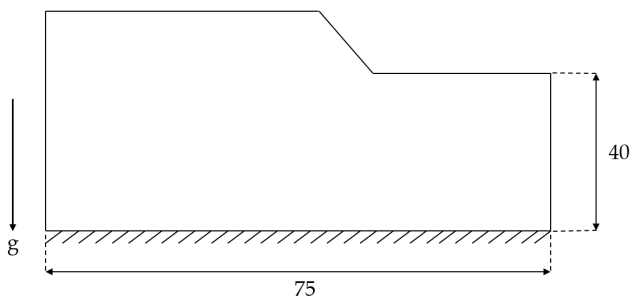
\includegraphics[width=0.5\textwidth]{images/benchmark_slope/rama16c}
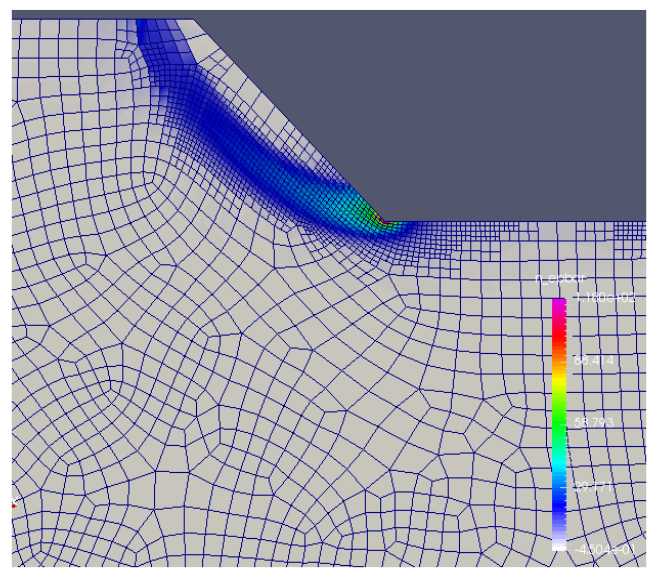
\includegraphics[width=0.4\textwidth]{images/benchmark_slope/rama16b}\\
{\captionfont Left: Slope stability problem setup; Right: Adaptive Refinement based 
on Plasticity Indicator}
\end{center}


%..............................................................................
\subsubsection{Time-dependent benchmark in an annulus}\label{sec:tdba}

This benchmark is presented in Gass{m\"o}ller \etal \cite{galb19}.
The domain is a 2D annulus with inner and outer radii $R_1=1$ and $R_2=2$, respectively.
In this situation, the incompressible isothermal Stokes equations and their solution
can be expressed in a cylindrical coordinate system in terms of the radius $r$ and the
azimuthal angle $\theta$. The viscosity is set to $eta=1$, and the density is given by
\begin{equation}
\rho(r,\theta)=48r^5
\end{equation}
The gravity vector is set to 
\begin{equation}
\vec{g}(r,\theta)=\frac{r^3}{384} \vec{e}_r + \vec{e}_\theta
\end{equation}
Note that this gravity vector is not the gradient of a gravity potential
and consequently not physical.
The Stokes system can then be solved using a separation of variables
approach and yields
\begin{equation}
\vec{\upnu}=-r^7 \vec{e}_\theta
\quad\quad
p(r,\theta)=\frac{r^9}{72}-\frac{512}{72}
\end{equation}
\begin{center}
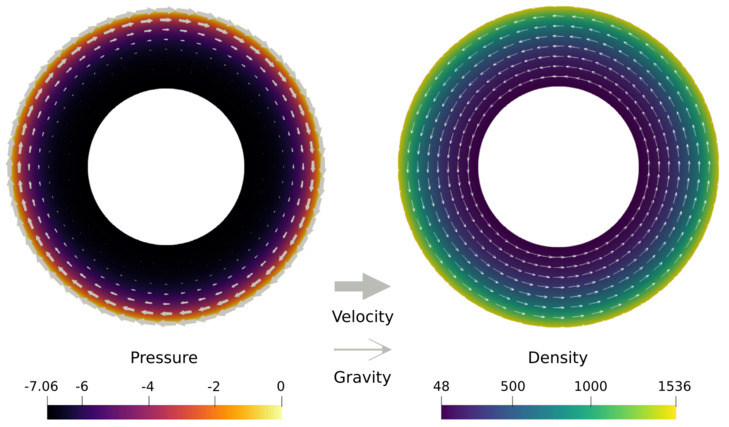
\includegraphics[width=12cm]{images/benchmark_annulus/galb19}\\
{\captionfont Taken from \cite{galb19}}
\end{center}
Rather importantly, this benchmark was arrived at by means of a stream function (see Section~\ref{sec:streamfunction}) 
$\psi(r,\theta)=F(r)G(\theta)$ with $F(r)=r^8/8$ and $G(\theta)=1$.

%..............................................................................
\subsubsection{Convection in 2D-box} \label{sec:citb}

We start from the following stream function (see Section~\ref{sec:streamfunction}):
\begin{equation}
\psi(x,y)=\frac{1}{\pi} \sin \pi x \sin \pi y
\end{equation}
which yields:
\begin{eqnarray}
u(x,y)&=&\frac{\partial \psi}{\partial y} = \sin \pi x \cos \pi y \nn\\
v(x,y)&=&-\frac{\partial \psi}{\partial x} = - \cos \pi x \sin \pi y
\end{eqnarray}
The pressure field is 
\begin{equation}
p(x,y) = 2\pi \cos (\pi x) \cos (\pi y) 
\end{equation}
with 
\begin{equation}
\rho(x,y)=\sin(\pi x) \sin (\pi y)
\qquad\qquad
g_y = -4\pi ^2 \frac{\cos (\pi x)}{\sin (\pi x)}
\end{equation}

\begin{center}
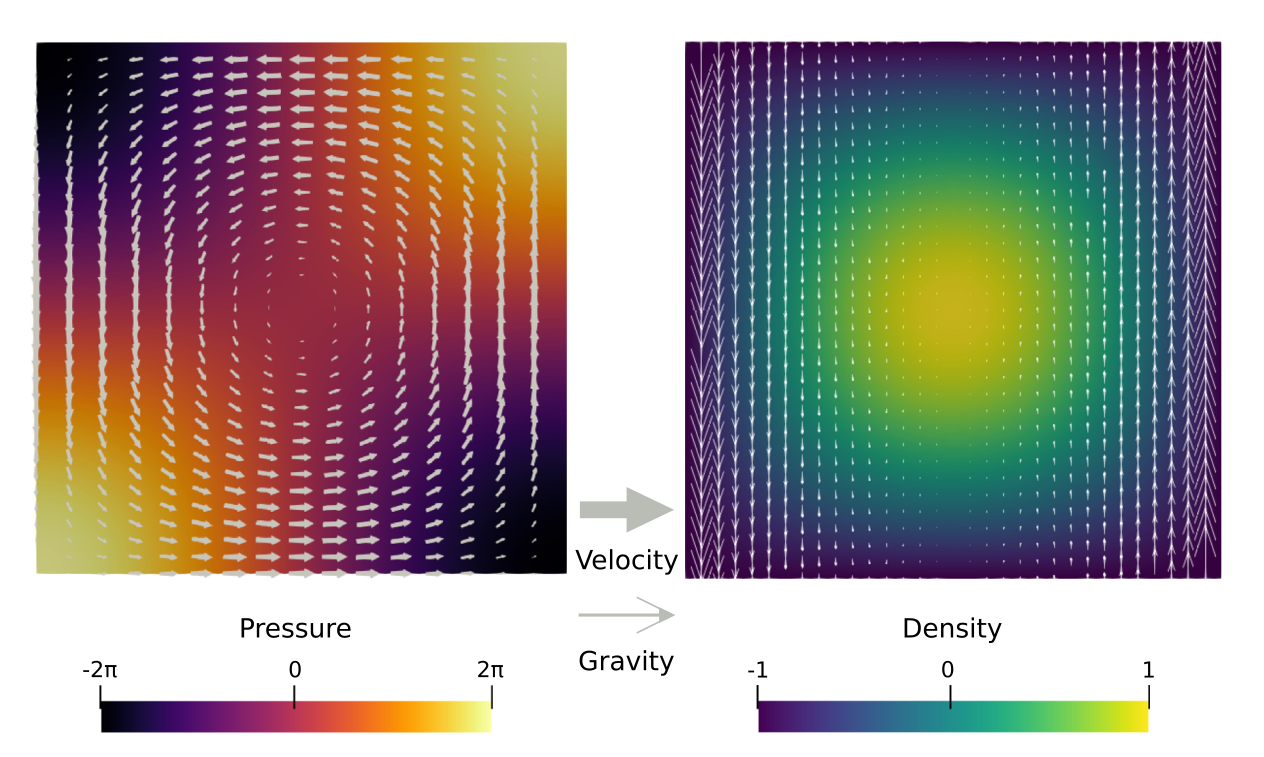
\includegraphics[width=12cm]{images/benchmark_convbox/galb19}\\
{\captionfont Taken from \cite{galb19}}
\end{center}

\begin{eqnarray}
v_{rms} 
&=& \sqrt{\frac{1}{L_xL_y} \int_0^1 \int_0^1 (u^2+v^2) dxdy} \nn\\
&=& \sqrt{\int_0^1 \int_0^1 ( \sin^2 (\pi x) \cos^2 (\pi y) + \cos^2 (\pi x) \sin^2 (\pi y) ) dxdy} \nn\\
&=& \sqrt{ \int_0^1 \sin^2 (\pi x) dx  \cdot \int_0^1 \cos^2 (\pi y) dy + \int_0^1 \cos^2 (\pi x) dx \cdot \int \sin^2 (\pi y) dy } \nn\\
&=& \sqrt{\frac{1}{2} \frac{1}{2}+ \frac{1}{2} \frac{1}{2} }\nn\\
&=& \frac{\sqrt{2}}{2} \nn\\
&\simeq& 0.70711...
\end{eqnarray}


%..............................................................................
\subsubsection{The sinker problem}\label{sec:sinker}

This experiment is not a benchmark stricto sensu since there is no analytical solution. However, it is widely used in the technical literature because of its simple setup and since it allows to test solving strategies.
Also, it can conveniently be carried out in both two and three dimensions.

\paragraph{In two dimensions} The time dependent version of the experiment is for instance to be found 
in Gerya \cite{gery10} and the same is repeated in Thieulot \cite{thie11}.

This simple benchmark provides challenging numerical experiments 
dealing with large viscosity variations within the simulation
domain. It consists of a bulk of fluid 1 ($\eta_1,\rho_1$) 
in which a block of fluid 2 ($\eta_2,\rho_2$) falls under its own
weight. The domain is a square of size $L_x = L_y = 500\si{\kilo\metre}$ and the
block is initially centred at point ($x=250\si{\km}$, $y=400\si{\km}$) with size
$100 \times 100\si{\km}$.
Free slip boundary conditions are imposed on all sides of the domain. 
In \cite{thie11} five experiments have been conducted:
$\eta_1 = 10^{20}\si{\pascal\second}$, $\rho_2=3220\si{\kg\per\cubic\metre}$ ;
$\eta_1 = 10^{21}\si{\pascal\second}$, $\rho_2=3300\si{\kg\per\cubic\metre}$ ;
$\eta_1 = 10^{22}\si{\pascal\second}$, $\rho_2=6600\si{\kg\per\cubic\metre}$ ;
$\eta_1 = 10^{23}\si{\pascal\second}$, $\rho_2=3300\si{\kg\per\cubic\metre}$ ;
$\eta_1 = 10^{24}\si{\pascal\second}$, $\rho_2=9900\si{\kg\per\cubic\metre}$ ;
while in all experiments the density of the surrounding fluid is
$\rho_1=3200\si{\kg\per\cubic\metre}$ and the viscosity of the block is varied between
$10^{19}$ and $5\cdot10^{27}\si{\pascal\second}$.

\begin{center}
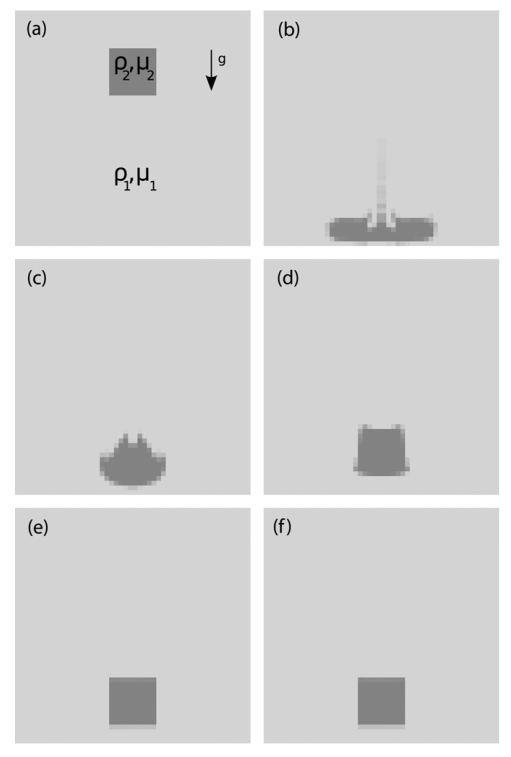
\includegraphics[width=5cm]{images/benchmark_sinker/thie11a}
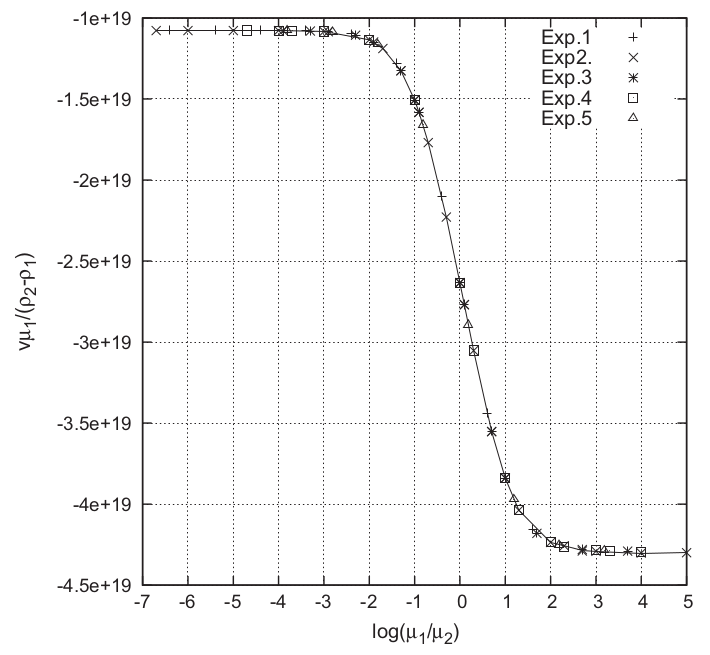
\includegraphics[width=7cm]{images/benchmark_sinker/thie11b}\\
{\captionfont Left: 
$\eta_1 = 10^{21}\si{\pascal\second}$, $\rho_2= 3300\si{\kg\per\cubic\metre}$. 
(a) Initial setup; 
(b) $\eta_1 = 10^{21}\si{\pascal\second}$ at time $t$ = 10 Myrs; 
(c) $\eta_1 = 10^{22}\si{\pascal\second}$ at time $t$ = 20 Myrs; 
(d) $\eta_1 = 10^{23}\si{\pascal\second}$ at time $t$ = 20 Myrs; 
(e) $\eta_1 = 10^{25}\si{\pascal\second}$ at time $t$ = 20 Myrs; 
(f) $\eta_1 = 10^{27}\si{\pascal\second}$ at time $t$ = 20 Myrs. 
Right: Velocity measurements as a function of the viscosity contrast between
surrounding medium and block for all experiments.
Taken from \cite{thie11}}
\end{center}

\paragraph{In three dimensions}
Let us look at the sinker experiment from Furuichi \etal \cite{fumt11}: 
The domain is the unit box the origin at the center of the box. A cube with a viscosity $\eta_1=\Delta \eta$ 
and density $\rho_1 = 1$ was placed at the middle of the domain defined by
$-0.15 \leq x,y,z \leq 0.15$.
The material surrounding the cube has the properties $\eta_0=1$ and $\rho_0 = 0$. 
The body force of the momentum equation was taken as $(0, 0,-\rho g)$ with $g = 1$.
Along all walls on the domain, free-slip boundary conditions were employed.

\begin{center}
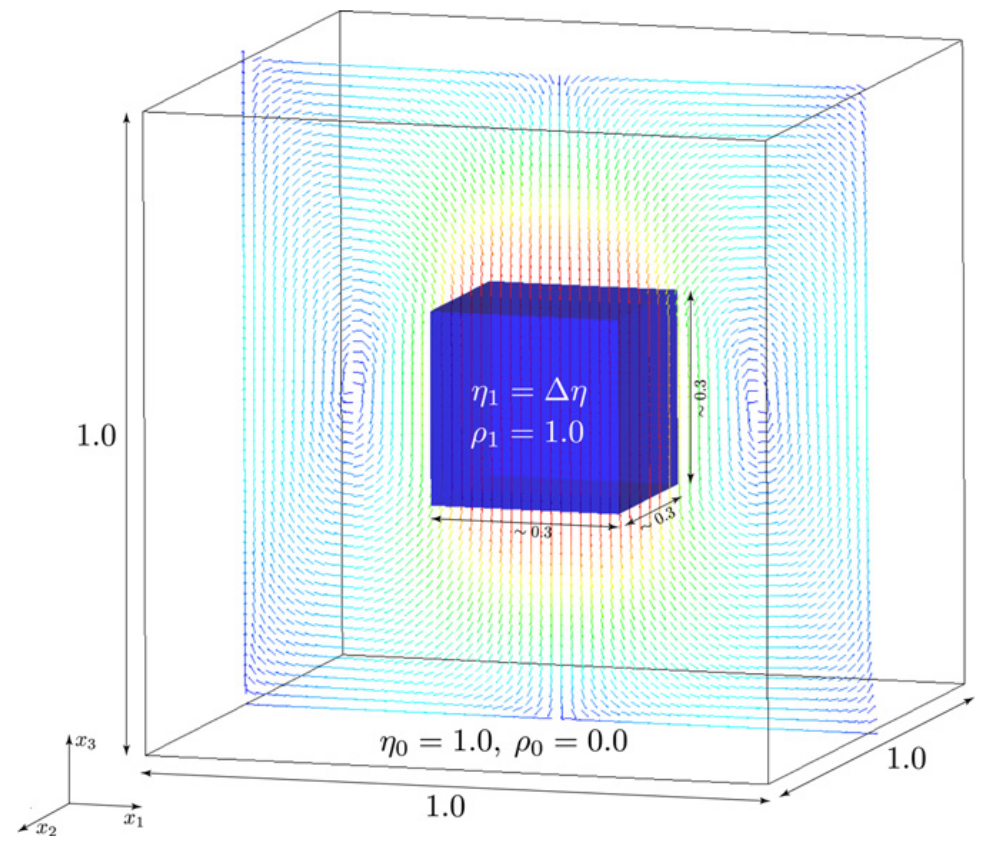
\includegraphics[width=6cm]{images/benchmark_sinker/fumt11}\\
{\captionfont Simulation setup for the 3D falling block (SINKER) problem. The vectors represent computed flow.
Taken from \cite{fumt11}}
\end{center}


%.......................................................
\paragraph{Sinking block results for multiple elements}

The setup is slightly altered: the domain is 512x512km. 
The block has size $L_b\times L_b=128\times 128$km, and is centered
on ($L_x/2,3L_y/4$). Free slip on all sides. Pressure is volume normalised. $|g_y|=10$.
This benchmark is part of \aspect, and can therefore be run with $Q_2\times Q_1$, $Q_2\times P_{-1}$ and $Q_1\times P_0$ elements (although the solver does not converge for the latter at high resolutions).
Velocity and pressure are measured in the middle of the block (in the case of the $Q_1^+\times P_0$ element the 
projected pressure $q$ on the $Q_1$ is used).

As above, the quantity $|v|\eta_1/\delta\rho$velocity is considered, but this time plotted as a function 
of the resolution for a fixed $\eta_2$ and for various element types. The quantity $p/\delta\rho/L_b$
is also plotted:

\begin{center}
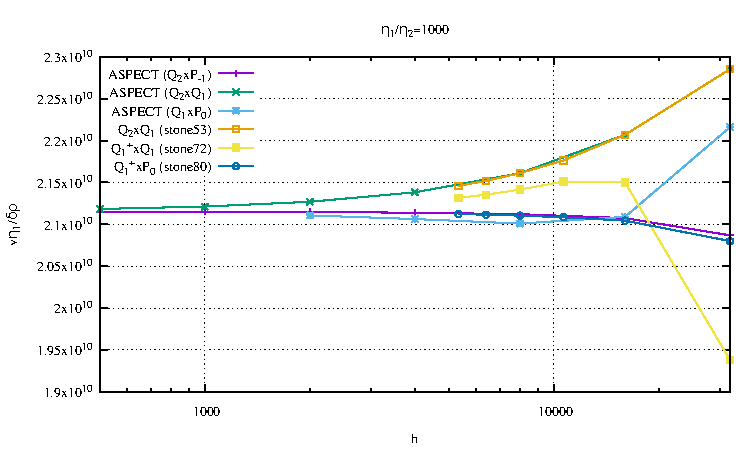
\includegraphics[width=7.9cm]{images/benchmark_sinkingblock/eta2_1e18/v.pdf}
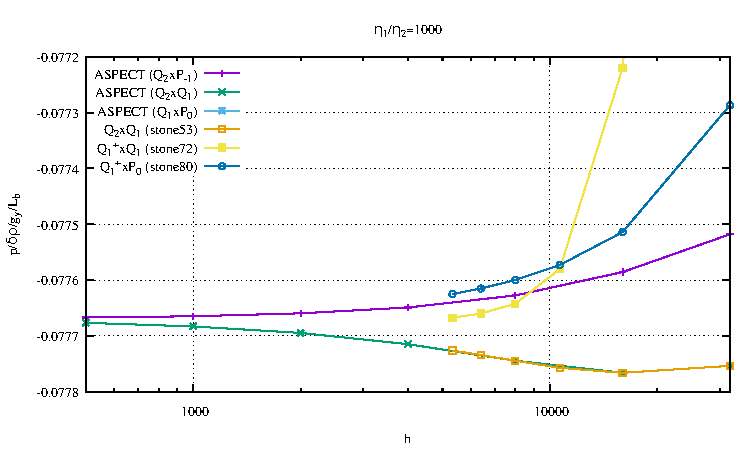
\includegraphics[width=7.9cm]{images/benchmark_sinkingblock/eta2_1e18/p.pdf}\\
{\captionfont Results for $\rho_1=0$, $\rho_2=\delta\rho=8$, $\eta_1=10^{21}$ and $\eta_2=10^{18}$}
\end{center}

\begin{center}
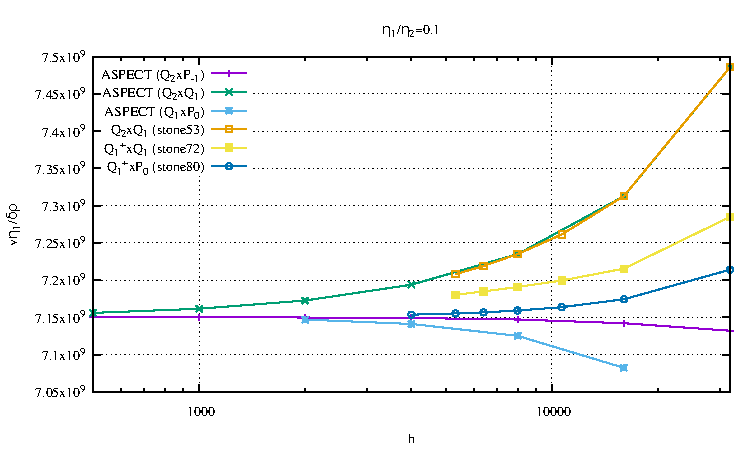
\includegraphics[width=7.9cm]{images/benchmark_sinkingblock/eta2_1e22/v.pdf}
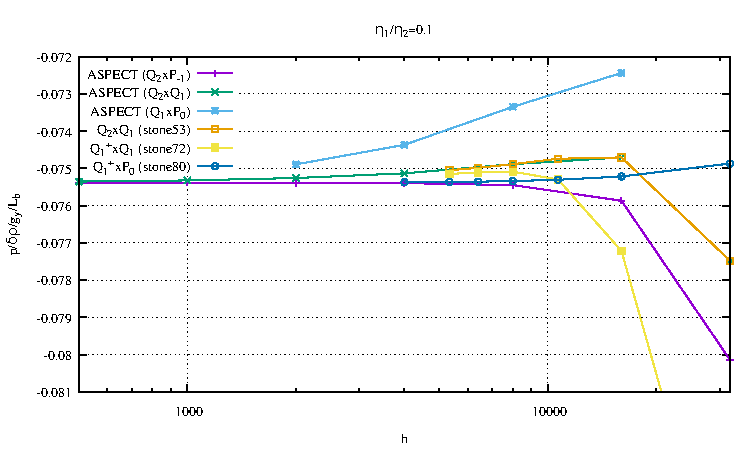
\includegraphics[width=7.9cm]{images/benchmark_sinkingblock/eta2_1e22/p.pdf}\\
{\captionfont Results for $\rho_1=0$, $\rho_2=\delta\rho=8$, $\eta_1=10^{21}$ and $\eta_2=10^{22}$}
\end{center}

Results obtained with \aspect with $\rho_1=3200$ and $\rho_2=\rho_1+\delta\rho$ are shown here:

\begin{center}
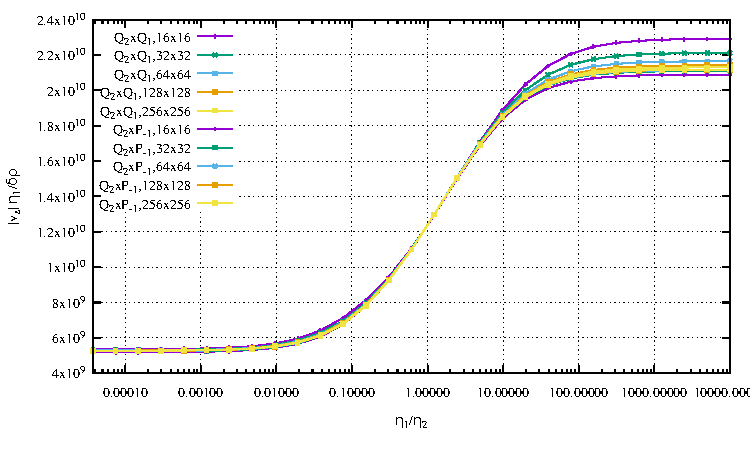
\includegraphics[width=12cm]{images/benchmark_sinkingblock/aspect/v.pdf}
\end{center}


%......................................................
\subsubsection{The hot blob problem}\label{sec:hotblob}

This is a very similar setup as the 3D sinker from the same authors
with higher but more diffusive variation of viscosity.
The body force is given by $(0, 0, \beta T)$ and
where the temperature field $T$ is defined by $T = \exp  (-\gamma (x^2+y^2+(z-0.3)^2))$ 
with the constant parameters $\beta=10^6$ and $\gamma=200$. 
The temperature-dependent viscosity $\eta = \exp( -\alpha T)$ is employed with the parameter for viscosity
contrast $\alpha$.

\begin{center}
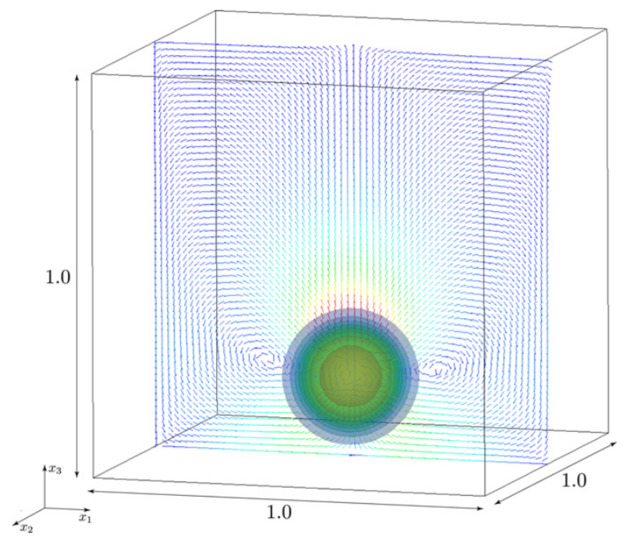
\includegraphics[width=8cm]{images/benchmark_hotblob/fumt11}\\
{\captionfont Simulation setting of BLOB problem. Isosurface and vectors represent temperature field \\and computed flow respectively. Taken from \cite{fumt11}}
\end{center}

%...........................................................
\subsubsection{The punch/indentor problem in 2D} \label{sec:punch}

The punch benchmark is one of the few boundary value problems involving plastic solids 
for which there exists an exact solution. 
Such solutions are usually either for highly simplified geometries (spherical or axial 
symmetry, for instance) or simplified material models (such as rigid plastic solids) \cite{kacha04}.

In this experiment, a rigid punch indents a rigid plastic half space; the slip line field theory gives 
exact solutions as shown hereunder:

\begin{center}
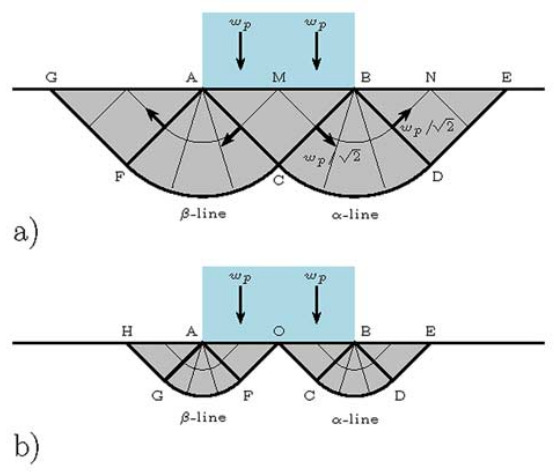
\includegraphics[width=6cm]{images/benchmark_punch/thfb08}\\
{\captionfont Two-dimensional rigid punch indenting a rigid
plastic half space. (a) Prandtl’s rigid plastic solution; (b)
Hill’s solution. Taken from \cite{thfb08}}
\end{center}

The plane strain formulation of the equations and the detailed solution to the problem 
were derived in the Appendix of \cite{thfb08} and are also presented in \cite{gepd98} 
and in \cite[Chapt.6]{bower2009}.
The two dimensional punch problem has been extensively studied numerically for the past 40 years 
\cite{zihl75,prlo90,zihp95,ziph95,chpe01,chan99,huhy99,yuti06,bufs08,raab07,gltf18} and has been used to draw a parallel with the tectonics of eastern China in the context of the 
India-Eurasia collision \cite{tamo76,mota77,engl82} or the European Alps \cite{repe97}.
It is also worth noting that it has been carried out in one form or another in series of 
analogue modelling articles concerning the same region, with a rigid indenter colliding with a rheologically 
stratified lithosphere \cite{tapl82,peta88,daco88,jodc90}.


\begin{center}
a)\includegraphics[width=5cm]{images/benchmark_punch/gps}
b)\includegraphics[width=5cm]{images/benchmark_punch/img5}
c)\includegraphics[width=5cm]{images/benchmark_punch/img7}\\
d)\includegraphics[width=5cm]{images/benchmark_punch/img6}
e)\includegraphics[width=5cm]{images/benchmark_punch/img8}
f)\includegraphics[width=5cm]{images/benchmark_punch/img11}\\
{\captionfont b,c) Model by Tapponnier \etal (1982) \cite{tapl82} or 
Peltzer \& Tapponnier (1988) \cite{peta88}. Not sure about source for other figures.}
\end{center}


 
Numerically, the one-time step punch experiment is performed on a two-dimensional
domain of purely plastic von Mises material. 
Given that the von Mises rheology yield criterion does not depend on pressure, the density of the material and/or the gravity vector is set to zero. Sides are set to free slip boundary conditions, the bottom to no slip, while a vertical velocity $(0,-v_p)$ is prescribed at the top boundary for nodes whose $x$ coordinate is within $[L_x/2-\delta/2,L_x/2+\delta/2]$. 

The analytical solution predicts that the angle of the shear bands stemming from the sides of the punch 
is $\pi/4$, that the pressure right under the punch is $1+\pi$, 
and that the velocity of the rigid blocks on each side of the punch is $v_p/\sqrt{2}$ 
(this is simply explained by invoking conservation of mass).


\begin{center}
\includegraphics[width=10cm]{images/benchmark_punch/gltf18}\\
{\captionfont The punch benchmark results after 500 nonlinear iterations for a rough punch (left column) 
and a smooth punch (right column). (a,f) Viscosity field with analytical slip lines. 
(b,g) Strain rate norm $\dot\varepsilon_e$ with measured shear band angles. 
(c,h) Velocity magnitude with velocity vectors along the surface of the domain.
(d,i) Pressure field. (e,j) Pressure along the surface of the domain (colored line) and analytical 
solution values $\pi + 1$ and 1 (grey lines). Taken from \cite{gltf18}}
\end{center}

\begin{remark}
This benchmark is often mentioned or used in the context of bearing capacity, footings, 
limit state design/analysis \cite{mich01,zhll03,gour04,gork06,lesk05,shls03}.
\end{remark}


%................................................................................
\subsubsection{Driven cavity with analytical solution} \label{sec:ldc_anal}

This comes from Elman \etal \cite{elsw}(section 3.1.4)\footnote{actually, not?}. The velocity is prescribed to be
\[
{\vec v}=(2y(1-x^2) ; -2x(1-y^2) )
\]
on the domain $\Omega=[-1:1]\times[-1:1]$. The strainrate tensor is given by:
\[
\dot{\bm \varepsilon}=
\left(
\begin{array}{cc}
-4xy & -x^2+y^2  \\
-x^2+y^2 & 4xy   
\end{array}
\right)
\]
The Stokes equation is then:
\begin{eqnarray}
-\frac{\partial p}{\partial x} + 2\eta ( -4y + 2y ) &=& \rho g_x \\
-\frac{\partial p}{\partial y} + 2\eta ( -2x + 4x ) &=& \rho g_y
\end{eqnarray}
where we assume the viscosity $\eta=1$ to be constant in space.
Assuming $g_x=0$, the first equation is
\[
\frac{\partial p}{\partial x} = - 4 y
\]
i.e.
\[
p(x,y)= -4  y x +f(y)
\]
Inserting this in the second equation:
\[
4  x - f'(y) + 4 x  = \rho g_y
\]
or,
\[
-f'(y) + 8  x  = \rho g_y
\]
Assuming $g_y=-1$, we get $\rho=-8x$ and then $f'(y)=0$ so $f(y)=C$ where $C$
is a constant.
Finally the pressure is given by:
\[
p(x,y)=-4  y x + C
\]
We add the following requirement: $\int_\Omega p(x,y) d\Omega =0$ so that $C=0$.

\begin{center}
\includegraphics[width=6cm]{images/benchmark_ldc_anal/velo}
\includegraphics[width=6cm]{images/benchmark_ldc_anal/press}
\end{center}

\begin{eqnarray}
v_{rms}^2 
&=& \frac{1}{\Omega} \int_\Omega (u^2+v^2) d\Omega \nonumber\\
&=& \frac{1}{4} \int_{-1}^{+1}\int_{-1}^{+1} (u^2+v^2) dxdy \nonumber\\
&=& \frac{1}{4} \int_{-1}^{+1}\int_{-1}^{+1} [ 4y^2(1-x^2)^2 + 4x^2(1-y^2)^2   ] dxdy \nonumber\\
&=& \int_{-1}^{+1}\int_{-1}^{+1} [ y^2(1-x^2)^2 + x^2(1-y^2)^2   ] dxdy \nonumber\\
&=& \int_{-1}^{+1}\int_{-1}^{+1} [ y^2(1-2x+x^2) + x^2(1-2y+y^2)  ] dxdy \nonumber\\
&=& \int_{-1}^{+1}\int_{-1}^{+1} y^2 dxdy
+ \int_{-1}^{+1}\int_{-1}^{+1} 2 x^2 y^2 dxdy
+ \int_{-1}^{+1}\int_{-1}^{+1} x^2 dxdy\nn\\
&=& 2  \frac23 + 2 \frac23\frac23 + 2 \frac23 \nn\\
&=& \frac{32}{9} \nn\\
&=& 3.5555
\end{eqnarray}

We can reformulate the benchmark in the unit square $\Omega=[0:1]\times[0:1]$.

\begin{eqnarray}
u(x,y) &=&  (2y-1)x(1-x) \nn\\
v(x,y) &=& - (2x-1)y(1-y) \nn
\end{eqnarray}

Then 
\begin{eqnarray}
\dot\varepsilon_{xx}(x,y) &=& (2y-1)(1-2x) \nn\\
\dot\varepsilon_{xy}(x,y) &=&  x(1-x)  - y(1-y)  \nn\\
\dot\varepsilon_{yy}(x,y) &=& - (2x-1)(1-2y)  \nn
\end{eqnarray}
We of course recover 
\[
\dot\varepsilon_{xx}(x,y) + \dot\varepsilon_{yy}(x,y) = 0
\]
The Stokes equation is then:
\begin{eqnarray}
-\frac{\partial p}{\partial x} + 2\eta (-2(2y-1)-(1-2y)  ) &=& \rho g_x \nn\\
-\frac{\partial p}{\partial y} + 2\eta ((1-2x)+2(2x-1)  ) &=& \rho g_y \nn
\end{eqnarray}
or
\begin{eqnarray}
-\frac{\partial p}{\partial x} + 2\eta (1-2y) &=& \rho g_x \nn\\
-\frac{\partial p}{\partial y} - 2\eta (1-2x) &=& \rho g_y \nn
\end{eqnarray}
where we assume the viscosity $\eta=1$ to be constant in space.
Assuming $g_x=0$, the first equation is
\[
\frac{\partial p}{\partial x} =  2 (1-2y)
\]
i.e.
\[
p(x,y) = 2 x (1-2y) + f(y)
\]
Inserting this in the second equation:
\[
4 x - f'(y) - 2 (1-2x)   = \rho g_y
\]
Assuming $g_y=-1$, then
\[
8 x -2  - f'(y)  = \rho 
\]
we set $\rho(x,y)= 8x-2$ and then $f'(y)=0$ so $f(y)=C$ where $C$
is a constant.
Finally the pressure is given by:
\[
p(x,y)= 2 x (1-2y) + C
\]
We add the following requirement: $\int_\Omega p(x,y) d\Omega =0$ 
\[
\int_{0}^1 \int _0^1 p(x,y) = 0
\Rightarrow 
\int_{0}^1 \int _0^1 [ 2 x (1-2y) + C] = 0
\]
so that $C=0$.

We also find $\upnu_{rms}=\frac{1}{\sqrt{45}}\simeq 0.1490711985$



%................................................................................
\subsubsection{Viscous flow around a cylinder in 2D and 3D } \label{sec:flowcyl}

There are many variants of this problem: 2D in Turek \cite{turek}, 3D in John \cite{john02}.
Many studies focus on Navier-Stokes flow since the cylinder generates
vortices at high Reynolds numbers. Steady state solutions at low Re are shown 
here\footnote{\url{up of the test and data measurement}}.
Note the interesting benchmark for 2D visco-elastic flow in Beuchert \& Podlachikov \cite{bepo10}.

\begin{center}
\includegraphics[width=8cm]{images/benchmark_flow_cylinder/turek}
\includegraphics[width=6cm]{images/benchmark_flow_cylinder/john02}\\
{\captionfont Left: taken from Turek \cite{turek}; Right: taken from John \cite{john02}}
\end{center}

\Literature: Tachibana \& Iemoto (1987) \cite{taie87}



%................................................................................
\subsubsection{Heat flow around a cylinder} \label{sec:hfcyl}

The domain is a 2D Cartesian box of size 8x4.
The Stokes equations are not solved and the following velocity is prescribed:
\begin{eqnarray}
u(x,y)&=& U_\infty \left(  1-\frac{x^2-y^2}{(x^2+y^2)^2}  \right) \\
v(x,y)&=& -2U_\infty \frac{xy}{(x^2+y^2)^2}
\end{eqnarray}
Boundary conditions are as follows:
$T=0$ is imposed at the top and bottom of the domain. 
$T=1$ is imposed inside a disc centered at (2,2) with radius 1.  
Further: $k=0.01$, $C_p=1$, $\rho=1$, CFL number is 0.1.

\begin{center}
\includegraphics[width=5cm]{images/benchmark_heatcyl/u}
\includegraphics[width=5cm]{images/benchmark_heatcyl/w}
\includegraphics[width=5cm]{images/benchmark_heatcyl/vel}
\end{center}

\begin{center}
\includegraphics[width=5cm]{images/benchmark_heatcyl/temper_0000}
\includegraphics[width=5cm]{images/benchmark_heatcyl/temper_0020}
\includegraphics[width=5cm]{images/benchmark_heatcyl/temper_0040}\\
\includegraphics[width=5cm]{images/benchmark_heatcyl/temper_0060}
\includegraphics[width=5cm]{images/benchmark_heatcyl/temper_0080}
\includegraphics[width=5cm]{images/benchmark_heatcyl/temper_0150}\\
{\captionfont Time evolution of the temperature field.
Results obtained with \elefant (unpublished)}
\end{center}

This is carried out in \stone 65.

%................................................................................
\subsubsection{Thermal diffusion of half-cooling space} \label{sec:hcsp}

This is a simple 1D experiment which solution is (for instance) available 
in Turcotte \& Schubert \cite{tusc} and is also presented in Choi \etal \cite{chtl13}.

The domain is 100km deep. $T_0=$0\degree C is prescribed a the surface and 
$T_m=$1300\degree C is prescribed at the bottom. The initial temperature is $T(y)=1300$\degree C.
The material is characterised by $\rho=1000$kg/m$^3$, $C_p=1000$J/kg/K, 
$k=1$J/m/K. The time-dependent solution is given by:
\begin{equation}
T(y,t)=T_0 + (T_0-T_m) \text{erf} \left( \frac{y}{2\sqrt{k t /\rho C_p}}  \right)
\end{equation}

\begin{center}
\includegraphics[width=6cm]{images/benchmark_hcsp/chtl13}\\
{\captionfont Thermal diffusion of half space cooling plate.
The temperature profiles in the analytical solution at 1, 5,
and 15 Myrs are plotted in solid lines. The results from
DynEarthSol2D are plotted in circles. Taken from \cite{chtl13}}
\end{center}


%................................................................................
\subsubsection{Laplace equation on a semi infinite plate} \label{sec:lapplate}
\begin{flushright} {\tiny {\color{gray} benchmark\_laplace\_plate.tex}} \end{flushright}

This experiment is based on a 2nd year mathematics lecture I give at Utrecht University. 
One wishes to solve the Laplace equation for temperature on the following plate subject 
to the indicated boundary conditions:

\begin{center}
\includegraphics[width=3.5cm]{images/benchmark_lapplate/laplace2.png}
\end{center}


The temperature satisfies the 2D Laplace equation inside the plate:
\begin{equation}
\frac{\partial^2 T}{\partial x^2}
+ \frac{\partial^2 T}{\partial y^2} = 0
\end{equation}

We could try to solve the equation by using a tentative solution of the form:
\begin{equation}
T(x,y)=\theta(x) \Phi(y)
\end{equation}

\includegraphics[width=.5cm]{images/benchmark_lapplate/warning.png}
We do not {\it know} the solution is of this form.

We substitute (2) into (1) and obtain:
\[
\Phi \frac{\partial^2 \theta}{\partial x^2} +
\theta \frac{\partial^2 \Phi}{\partial y^2} = 0
\]
Dividing by $\theta\Phi$ gives:
\[
\frac{1}{\theta} \frac{\partial^2 \theta}{\partial x^2} +
\frac{1}{\Phi} \frac{\partial^2 \Phi}{\partial y^2} = 0
\]

Separation of variables: we say that each term is a constant because the first term is a function of $x$ only
and the second a function of $y$ only.
We then write
\[
\frac{1}{\theta} \frac{\partial^2 \theta}{\partial x^2} = - \frac{1}{\Phi} \frac{\partial^2 \Phi}{\partial y^2} = -k^2
\]
where $k$ is called the separation constant.
This leads to 
\[
\frac{\partial^2 \theta}{\partial x^2} + k^2 \theta = 0
\]
\[
\frac{\partial^2 \Phi}{\partial y^2} - k^2 \Phi =0
\]

\begin{itemize}
\item The solution to the first one is $\theta(x)=\sin kx$ or $\theta(x)=\cos kx$
\item The solution to the second one is $\Phi(x)=e^{kx}$ or $\Phi(x)=e^{-kx}$
\end{itemize}


The general solution writes:

\[
T(x,y)=\theta(x) \Phi(y)=
\left\{
\begin{array}{c}
\sin kx \\ \cos kx
\end{array}
\right\}
\left\{
\begin{array}{c}
e^{ky} \\ e^{-ky}
\end{array}
\right\}
\]

We can now use the b.c. to find the solution to the Laplace equation.

\begin{itemize}
\item Since $T\rightarrow 0$ when $y\rightarrow \infty$ then $e^{ky}$ unacceptable.
\item Since $T=0$ when $x=0$ then $\cos kx$ unacceptable.
\end{itemize}

so
\[
T(x,y)=
\sin (kx)  \;
 e^{-kx}
\]

We finally use $T=0$ at $x=10$ which leads to $10k=n \pi$, i.e.:

\[
T(x,y)=\sin (\frac{n\pi x}{10}) \;   e^{-n\pi y/10}
\]

\includegraphics[width=.5cm]{images/benchmark_lapplate/warning.png}
Problem: the solution does not satisfy  $T(x,0)=100$.
However, a linear combination of solutions is still a solution !
Let's find such a combination which satisfies the b.c. at $y=0$ :
\[
T(x,y) = \sum_{n=1}^\infty b_n \sin (\frac{n\pi x}{10}) \;   e^{-n\pi y/10}
\]

We impose then $T(x,0)=100$:
\[
100 = \sum_{n=1}^\infty b_n \sin (\frac{n\pi x}{10}) 
\]
This is the Fourier sine series of $f(x)=100$ with $l=10$ (chapter 7.9 of Boas).

The coefficient $b_n$ is then given by
\[
b_n=\frac{2}{l} \int_0^l f(x) \sin\frac{n \pi x}{l} dx
=\frac{2}{10} \int_0^l 100 \sin\frac{n \pi x}{10} dx
=
\left\{
\begin{array}{ll}
400/n\pi & {\rm odd \; n} \\
0 & {\rm even \; n} \\
\end{array}
\right.
\]

Finally (!):
\[
T(x,y) = 
\frac{400}{\pi}
\left(
e^{-\pi y/10} \sin (\frac{\pi x}{10})
+\frac{1}{3}
\sin (\frac{3\pi x}{10}) \;   e^{-3\pi y/10}
+ \dots
\right)
\]

The simulation has been run with a 10x50 domain. All coefficients of the temperature equation are
set to 1, and the Stokes equation is not solved. The timestep is fixed to $dt=0.1$. Resolution 
is 32x160. 

\begin{center}
a)
\includegraphics[width=1.8cm]{images/benchmark_lapplate/temper0000.png}
\includegraphics[width=1.8cm]{images/benchmark_lapplate/temper0010.png}
\includegraphics[width=1.8cm]{images/benchmark_lapplate/temper0020.png}
\includegraphics[width=1.8cm]{images/benchmark_lapplate/temper0030.png}
\includegraphics[width=1.8cm]{images/benchmark_lapplate/temper0040.png}
\includegraphics[width=1.8cm]{images/benchmark_lapplate/temper0050.png}
\includegraphics[width=1cm]{images/benchmark_lapplate/colourscale.png}
\hspace{.2cm}
b)\includegraphics[width=1.8cm]{images/benchmark_lapplate/temper_analytical.png}\\
{\captionfont a) time evolution of the temperature field; b) analytical steady state solution}
\end{center}






%................................................................................
\subsubsection{Slab detachment benchmark} \label{sec:slabdetach}

\Literature: Schmeling (2011) \cite{schm11}, \aspect manual \cite{aspectmanual}, Glerum \etal \cite{gltf18}, 
\stone 26.

\begin{center}
\includegraphics[width=6cm]{images/benchmark_slabdetach/gltf18}\\
{\captionfont The detachment benchmark model setup of Schmalholz \cite{schm11}: 
a symmetric system of nonlinear viscous lithosphere with a vertical slab extending into a linear 
viscous mantle. The top and bottom boundaries are free slip, while the vertical boundaries are no slip.
Taken from \cite{gltf18}.}
\end{center}

%................................................................................
\subsubsection{Layered flow with viscosity contrast} \label{sec:layfl}

The idea behind this benchmark is to construct an analytical solution to the incompressible
Stokes equation in the case where the viscosity field showcases a 
viscosity contrast at location $y=y_0$ whose amplitude and width can be controlled. 
The viscosity is defined as
\[
\eta(y)=\frac{1}{\frac{1}{\pi} \tan^{-1} (\frac{y-y_0}{\beta} ) + 1/2 + \epsilon}
\]
where $\beta$ and $\epsilon$ are parameters. 

\begin{center}
\includegraphics[width=7cm]{images/benchmark_layeredflow/viscosityA}
\includegraphics[width=7cm]{images/benchmark_layeredflow/viscosityB}\\
\includegraphics[width=7cm]{images/benchmark_layeredflow/viscosityC}
\includegraphics[width=7cm]{images/benchmark_layeredflow/viscosityD}\\
{\captionfont Viscosity profiles for different values of $\beta$ and $\epsilon$ 
for $y_0=1/3$.
When $\beta$ is very large, the viscosity 
essentially converges to $\sim (1/2 + \epsilon)^{-1}$. 
$\beta$ controls the width of the transition while $\epsilon$ controls the amplitude 
of the viscosity variation.}
\end{center}

The flow is assumed to take place in an infinitely long pipe (in the horizontal direction)
and bound by 
$y=-1$ and $y+1$.
At the bottom we impose $v_x(y=-1)=0$ while we impose $v_x(y=+1)=1$ at the top.
The density is set to 1 while the gravity is set to zero.
Under these assumptions, the flow velocity and pressure fields are given by:
\begin{eqnarray}
v_x(x,y)&=&\frac{1}{2\pi} \left(  -\beta C_1 \log [\beta^2 + (z-y_0)^2]  + 2 (z-y_0)  C_1 \tan^{-1} \frac{z-y_0}{\beta} + \pi (1+2\epsilon) z C_1  + C_2 \right) \nonumber\\
v_y(x,y) &=& 0 \nonumber\\ 
p(x,y) &=& 0 
\end{eqnarray}
where $C_1$ and $C_2$ are integration constants:
\begin{eqnarray}
C_1 &=& 2\pi \left[ 
 \beta  \log [\beta^2 + (1+y_0)^2]  -  2(1+y_0) \tan^{-1} \frac{1+y_0}{\beta} 
-\beta  \log [\beta^2 + (1-y_0)^2]  +  2(1-y_0) \tan^{-1} \frac{1-y_0}{\beta} + 2\pi (1+2\epsilon)   \right]^{-1} \nonumber\\
C_2 &=&  \left[ \beta  \log [\beta^2 + (1+y_0)^2]  -  2(1+y_0) \tan^{-1} \frac{1+y_0}{\beta} + \pi(1+2\epsilon) \right]C_1, 
\end{eqnarray}

\begin{center}
\includegraphics[width=7cm]{images/benchmark_layeredflow/layeredflow_vel}
\includegraphics[width=7cm]{images/benchmark_layeredflow/layeredflow_viscosity}\\
{\captionfont Velocity and viscosity fields}
\end{center}

\paragraph{Analytical derivations} 
The flow takes place in the horizontal direction and is infinite in the this direction too so that:
\[
\vec\upnu=(u(y),0)
\]
The strain rate tensor is then given by:
\[
\dot{\bm \varepsilon}=
\frac{1}{2}
\left(
\begin{array}{cc}
0 & du/dy \\
du/dy & 0
\end{array}
\right)
\]
The momentum equation then becomes:
\[
{\vec \nabla} \cdot (2 \eta \dot{\bm \varepsilon} ) -{\vec \nabla}p 
=
{\vec \nabla} \cdot \left[ \eta(y) 
\left(
\begin{array}{cc}
0 & du/dy \\
du/dy & 0
\end{array}
\right)
\right] -{\vec \nabla}p 
= \rho {\vec g}
\]
On the vertical axis, when the gravity is zero, the equation is automatically verified when the 
pressure is zero.
On the horizontal axis:
\[
\frac{d}{dy} \left(\eta(y) \frac{du}{dy} \right) = 0
\]
Then 
\[
\eta(y) \frac{du}{dy}  = C_1
\]
or,
\[
\frac{du}{dy}  = \frac{C_1}{\eta(y)} = C_1 \left(\frac{1}{\pi} \tan^{-1} \frac{y-y_0}{\beta} 
+ 1/2 + \epsilon\right)
\]
so that the velocity is given by:
\[
u(y) = \frac{1}{\pi} ( y \tan^{-1}((y-y_0)/\beta) - y_0 \tan^{-1}((y-y_0)/\beta)  
-0.5* \beta \log (\beta^2 + y^2 - 2 y y_0 +y_0^2) + \pi y (\epsilon +0.5)) 
\]

\[
u(z)=\frac{1}{2\pi} \left(  -\beta C_1 \log [\beta^2 + (z-y_0)^2]  + 2 (z-y_0)  C_1 \tan^{-1} \frac{z-y_0}{\beta} + \pi (1+2\epsilon) z C_1  + C_2 \right)
\]
where $C_1$ and $C_2$ are integration constants.
I wish to impose $u(z=-1)=0$ and $u(z=+1)=1$:
\[
\frac{1}{2\pi} \left(  -\beta C_1 \log [\beta^2 + (-1-y_0)^2]  + 2 (-1-y_0)  C_1 \tan^{-1} \frac{-1-y_0}{\beta} - \pi (1+2\epsilon)  C_1  + C_2 \right) = 0
\]
\[
\frac{1}{2\pi} \left(  -\beta C_1 \log [\beta^2 + (1-y_0)^2]  + 2 (1-y_0)  C_1 \tan^{-1} \frac{1-y_0}{\beta} + \pi (1+2\epsilon)  C_1  + C_2 \right) = 1
\]
or,
\[
 -\beta C_1 \log [\beta^2 + (-1-y_0)^2]  + 2 (-1-y_0)  C_1 \tan^{-1} \frac{-1-y_0}{\beta} - \pi (1+2\epsilon)  C_1  + C_2 = 0
\]
\[
 -\beta C_1 \log [\beta^2 + (1-y_0)^2]  + 2 (1-y_0)  C_1 \tan^{-1} \frac{1-y_0}{\beta} + \pi (1+2\epsilon)  C_1  + C_2 = 2\pi
\]
or,
\[
 -\beta C_1 \log [\beta^2 + (-1-y_0)^2]  + 2 (1+y_0)  C_1 \tan^{-1} \frac{1+y_0}{\beta} - \pi (1+2\epsilon)  C_1  + C_2 = 0
\]
\[
 -\beta C_1 \log [\beta^2 + (1-y_0)^2]  + 2 (1-y_0)  C_1 \tan^{-1} \frac{1-y_0}{\beta} + \pi (1+2\epsilon)  C_1  + C_2 = 2\pi
\]
or,
\[
-\beta C_1 \log (\beta^2 + (1+y_0)^2)  +  2(1+y_0)C_1 \tan^{-1} ((1+y_0)/\beta) - \pi (1+2\epsilon)  C_1  +C_2  = 0
\]
\[
-\beta C_1 \log (\beta^2 + (1-y_0)^2)  +  2(1-y_0)C_1 \tan^{-1} ((1-y_0)/\beta) + \pi (1+2\epsilon)C_1  +C_2  = 2\pi
\]
I can now substract the first line from the second line:
\[
\beta C_1 \log (\beta^2 + (1+y_0)^2)  -  2(1+y_0)C_1 \tan^{-1} ((1+y_0)/\beta)  
-\beta C_1 \log (\beta^2 + (1-y_0)^2)  +  2(1-y_0)C_1 \tan^{-1} ((1-y_0)/\beta) + 2\pi (1+2\epsilon)C_1    = 2\pi
\]
i.e.,
\[
C_1= 2\pi \left[ 
 \beta  \log [\beta^2 + (1+y_0)^2]  -  2(1+y_0) \tan^{-1} [\frac{1+y_0}{\beta}] 
-\beta  \log [\beta^2 + (1-y_0)^2]  +  2(1-y_0) \tan^{-1} [\frac{1-y_0}{\beta}] + 2\pi (1+2\epsilon)   \right]^{-1}
\]
and then 
\[
C_2= \beta C_1 \log (\beta^2 + (1+y_0)^2)  -  2(1+y_0)C_1 \tan^{-1} ((1+y_0)/\beta) + \pi(1+2\epsilon) C_1 
\]



%\newpage

%\newpage
%For $\epsilon=0$

%\begin{center}
%\includegraphics[width=15cm]{viscosityA}\\
%\includegraphics[width=5cm]{velocity1}
%\includegraphics[width=5cm]{velocity3}
%\includegraphics[width=5cm]{velocity5}
%\end{center}

%\newpage
%For $\epsilon=0.1$

%\begin{center}
%\includegraphics[width=15cm]{viscosityB}\\
%\includegraphics[width=5cm]{velocity6}
%\includegraphics[width=5cm]{velocity8}
%\includegraphics[width=5cm]{velocity10}
%\end{center}



%................................................................................
\subsubsection{Elastic material in simple shear} \label{sec:elastsimpshear}

The domain is a Cartesian box of size $1\times1$. The boundary conditions are as follows:
\begin{itemize}
\item bottom: $u=v=0$
\item top: $u=1$, $v=0$
\end{itemize}
The shear modulus $\mu$ is set to 1, and the Poisson ratio $\nu$ is set to 0.25. 
Gravity is set to zero. 

The analytical solution for this problem is given by 
\[
\vec{\upnu}=
\left(
\begin{array}{c}
y \\
0 
\end{array}
\right)
\]
so that 
\[
\vec{\nabla}\vec{\upnu}=
\left(
\begin{array}{cc}
0 & 0 \\
1 & 0
\end{array}
\right)
\quad\quad
{\bm \varepsilon} = 
\frac{1}{2}
\left(
\begin{array}{cc}
0 & 1 \\
1 & 0
\end{array}
\right)
\]
The stress tensor then writes:
\[
{\bm \sigma}= \lambda \vec{\nabla}\cdot \vec{\upnu} + 2 \mu {\bm \varepsilon} 
= \mu 
\left(
\begin{array}{cc}
0 & 1 \\
1 & 0
\end{array}
\right)
\]
since $\vec{\nabla}\cdot \vec{\upnu}=0$.

The principal direction angle $\theta_p$ defines the principal
directions where the only stresses are normal stresses, and 
is given by the relationship:
\[
\tan (2\theta_p) =  \frac{2 \sigma_{xy}}{\sigma_{xx} -\sigma_{yy}}
\]
In our case the rhs is equal to $\infty$, which means that $2 \theta_p = \frac{\pi}{2}$
so that $\theta_p=\frac{\pi}{4}$.

The principal stresses are found from the original stresses via
\[
\sigma_{1,2}=\frac{\sigma_{xx}+\sigma_{yy}}{2} \pm \sqrt{  \left( \left(\frac{\sigma_x-\sigma_y}{2}\right)^2 +\sigma_{xy}^2  \right)}
\]
In our case 
\[
\sigma_{1,2} = \pm \sigma_{xy} = \pm \mu
\]
When plotting the principal stresses on the domain we expect crosses at 45\degree. 


%................................................................................
\subsubsection{Elastic material in pure shear} \label{sec:elastpureshear}

This is the same material as the previous benchmark but the boundary conditions are 
now as follows: $u=-1$ on the left, $u=1$ on the right, $v=1$ on the bottom and $v=-1$
on the top. 

In this case we have 
\[
u(x,y)=2(x-1/2) 
\qquad
v(x,y)=-2(y-1/2) 
\]
so 
\[
\vec{\nabla}\vec{\upnu}=
\left(
\begin{array}{cc}
2 & 0 \\
0 & -2
\end{array}
\right)
={\bm \varepsilon}
\]
and $\vec{\nabla}\cdot \vec{\upnu}=0$ so that 
the stress tensor then writes:
\[
{\bm \sigma}= \lambda \vec{\nabla}\cdot \vec{\upnu} + 2 \mu {\bm \varepsilon} 
= 2\mu 
\left(
\begin{array}{cc}
2 & 0 \\
0 & -2
\end{array}
\right)
\]

The principal direction angle $\theta_p$ defines the principal
directions where the only stresses are normal stresses, and 
is given by the relationship:
\[
\tan (2\theta_p) =  \frac{2 \sigma_{xy}}{\sigma_{xx} -\sigma_{yy}} = 0
\]
which means that $\theta_p = 0$.
Then the principal stresses are found from the original stresses via
\[
\sigma_{1,2}=\frac{\sigma_{xx}+\sigma_{yy}}{2} \pm \sqrt{  \left( \left(\frac{\sigma_x-\sigma_y}{2}\right)^2 +\sigma_{xy}^2  \right)}
\]
In our case 
\[
\sigma_{1,2} = \pm 4 \mu 
\]
When plotting the principal stresses on the domain we expect crosses which align with the axis. 






%................................................................................
\subsubsection{Uniform strip load on elastic material} \label{sec:elaststripload}

%\begin{center}
%\includegraphics[width=8cm]{ELASTOMECHANICS/UNIFORM_STRIP_LOAD/fig2}
%\end{center}

From Davis and Selvadurai \cite{dase96}(section 4.6) we have the components of the stress tensor:
\[
\sigma_{xx}=\frac{p_0}{\pi}\left[ \theta - \frac{1}{2}\sin 2\theta  \right]^{\theta_2}_{\theta_1}
\quad\quad\quad
\sigma_{zz}=\frac{p_0}{\pi}\left[ \theta + \frac{1}{2}\sin 2\theta  \right]^{\theta_2}_{\theta_1}
\quad\quad\quad
\sigma_{xz}=\frac{p_0}{\pi}\left[ \sin^2 \theta  \right]^{\theta_2}_{\theta_1}
\]
or, 
\begin{eqnarray}
\tilde{\sigma}_{xx}&=&\left[ \theta - \frac{1}{2}\sin 2\theta  \right]^{\theta_2}_{\theta_1} = \Theta - \frac{1}{2} ( \sin 2\theta_2 - \sin 2\theta_1) \nn\\
\tilde{\sigma}_{zz}&=&\left[ \theta + \frac{1}{2}\sin 2\theta  \right]^{\theta_2}_{\theta_1} = \Theta + \frac{1}{2} ( \sin 2\theta_2 - \sin 2\theta_1) \nn\\
\tilde{\sigma}_{xz}&=&\left[ \sin^2 \theta  \right]^{\theta_2}_{\theta_1} =  \sin^2 \theta_2 - \sin^2 \theta_1 \nn
\end{eqnarray}
with $\Theta=\theta_2-\theta_1$ and $\tilde{\sigma}_{ij}=\sigma_{ij}\pi/p_0$.
The (dimensionless) principal stresses are given by 
\[
\tilde{\sigma}_{1,2}=\frac{\tilde{\sigma}_{xx}+\tilde{\sigma}_{zz}}{2} \pm \sqrt{  \left(\frac{\tilde{\sigma}_{xx}-\tilde{\sigma}_{zz}}{2}\right)^2 +\tilde{\sigma}_{xz}^2 }
\]
We have
\begin{eqnarray}
\frac{\tilde{\sigma}_{xx}+\tilde{\sigma}_{zz}}{2} &=&  \Theta 
\nn\\
\frac{\tilde{\sigma}_{xx}-\tilde{\sigma}_{zz}}{2}
&=&  -\frac{1}{2} (  \sin 2\theta_2 - \sin 2\theta_1 ) \nn\\
&=&  -\frac{1}{2} ( 2 \cos (\theta_1+\theta_2) \sin \Theta ) \nn\\ 
&=&  -\cos (\theta_1+\theta_2) \sin \Theta  \nn\\ 
\tilde{\sigma}_{xz}
&=&\left[ \sin^2 \theta  \right]^{\theta_2}_{\theta_1}  \nn\\
&=&\sin^2 \theta_2 - \sin^2 \theta_1 \nn\\
&=&\frac{1}{2} (1-\cos \theta_2) - \frac{1}{2} (1-\cos 2\theta_1) \nn\\
&=& -\frac{1}{2} (\cos \theta_2 - \cos 2\theta_1) \nn\\
&=& -\frac{1}{2} ( -2 \sin (\theta_1+\theta_2) \sin(\theta_2-\theta_1) ) \nn\\
&=& \sin (\theta_1+\theta_2) \sin \Theta \nn
\end{eqnarray}
so that the principal stresses are finally given by
\[
\sigma_1 = \frac{p_0}{\pi} ( \Theta + \sin \Theta) 
\quad\quad\quad
\sigma_3 = \frac{p_0}{\pi} ( \Theta - \sin \Theta) 
\]
The principal stresses will be constant on any circle that passes through the edges of the 
strip load. It can also be shown that the direction of $\sigma_1$ points toward the highest 
point of this circle.

%\begin{center}
%\includegraphics[width=8cm]{ELASTOMECHANICS/UNIFORM_STRIP_LOAD/fig3}
%\end{center}


%................................................................................
\subsubsection{The annulus convection benchmark} \label{ss:anconv}

We wish to solve the Stokes equation in an annulus of inner radius $R_1$
and outer radius $R_2$ with the following boundary conditions:
\begin{itemize}
\item Inner boundary: $\upnu_r(R_1,\theta)=0$ 
\item Outer boundary: $\upnu_r(R_2,\theta)=0$ 
\end{itemize}
We then postulate
\[
v_\theta(r,\theta)= f(r) \cos(k\theta)
\]
Note that in the case $k=0$, we recover a constant velocity on the inner and outer boundaries.

The divergence of an incompressible vector field in polar coordinates is
\[
\frac{1}{r} \frac{\partial (r\upnu_r)}{\partial r} + \frac{1}{r} \frac{\partial v_\theta}{\partial \theta} =0
\]
or, 
\[
\frac{\partial (r\upnu_r)}{\partial r} + \frac{\partial v_\theta}{\partial \theta} =0
\]
i.e.,
\[
\frac{\partial (r\upnu_r)}{\partial r} = - \frac{\partial v_\theta}{\partial \theta} = k f(r) \sin(k\theta) 
\]
so 
\[
r\upnu_r(r,\theta) = k \left[ \int f(r) dr \right] \sin(k\theta) 
\]
and finally 
\[
\upnu_r(r,\theta) = k g(r) \sin(k\theta)  
\]
with 
\begin{eqnarray}
g(r)  &=& \frac{1}{r} \int f(r) dr \\
g'(r) &=& -\frac{1}{r^2} \int f(r) dr + \frac{1}{r} f = - \frac{1}{r} g + \frac{1}{r} f = \frac{1}{r}(f-g) 
\end{eqnarray}


The boundary conditions lead to
\[
\upnu_r(r=R_1,\theta) = 
k (\frac{A}{2}R_1 + \frac{B}{R_1} \ln R_1 + \frac{C}{R_1}) \sin(k\theta)  = 0
\]
\[
\upnu_r(r=R_2,\theta) = 
k (\frac{A}{2}R_2 + \frac{B}{R_2} \ln R_2 + \frac{C}{R_2}) \sin(k\theta)  = 0
\]
This has to be valid $\forall \theta$, so 
%\[
%\frac{A}{2}R_1^2 + B \ln R_1 - 1 =0 
%\]
%\[
%\frac{A}{2}R_2^2 + B \ln R_2 - 1 = 0
%\]
%or, 
\[
\frac{A}{2}R_1^2 + B \ln R_1 =-C
\quad\quad {\rm and} \quad\quad
\frac{A}{2}R_2^2 + B \ln R_2 =-C
\]
leading to 
\[
\frac{A}{2}+ \frac{B}{R_1^2} \ln R_1 =-\frac{C}{R_1^2}
\quad\quad {\rm and} \quad\quad
\frac{A}{2}+ \frac{B}{R_2^2} \ln R_2 =-\frac{C}{R_2^2}
\]
and finally 
\[
B = -C \frac{R_2^2-R_1^2}{R_2^2 \ln R_1 - R_1^2 \ln R_2}
\]
Likewise
\[
\frac{A}{2}R_1^2 + B \ln R_1 = -C
\quad\quad {\rm and} \quad\quad
\frac{A}{2}R_2^2 + B \ln R_2 = -C
\]
yields
\[
\frac{A}{2 \ln R_1}R_1^2 + B  = -\frac{C}{\ln R_1}
\quad\quad {\rm and} \quad\quad
\frac{A}{2 \ln R_2}R_2^2 + B  = -\frac{C}{\ln R_2}
\]
or, 
\[
\frac{A}{2 \ln R_1}R_1^2 - \frac{A}{2 \ln R_2}R_2^2  =  -C (\frac{1}{\ln R_1} - \frac{1}{\ln R_2})
\]
\[
A (\frac{R_1^2}{2 \ln R_1} - \frac{R_2^2}{2 \ln R_2})  =  -C (\frac{1}{\ln R_1} - \frac{1}{\ln R_2})
\]
\[
A (\frac{R_1^2 \ln R_2 }{2 } - \frac{R_2^2 \ln R_1 }{2} )  = -C( \ln R_2 - \ln R_1)
\]
finally
\[
A = -C\frac{2(\ln R_2 - \ln R_1)} { R_1^2 \ln R_2  - R_2^2 \ln R_1}    
= -C\frac{2(\ln R_1 - \ln R_2)} { R_2^2 \ln R_1  - R_1^2 \ln R_2}    
\]


We set ${\vec g}=-g_r {\vec e}_r$.
Stokes equation in Polar coordinates (p284 of Schubert, Turcotte and Olson book):
\begin{itemize}
\item 
$r$-component:
\[
\eta \left[ \nabla^2 \upnu_r - \frac{\upnu_r}{r^2} - \frac{2}{r^2} \frac{\partial u_\theta}{\partial \theta}  \right]
+
\frac{\eta}{3} \frac{\partial}{\partial r} \left[ \frac{1}{r}\frac{\partial (r \upnu_r)}{\partial r} + \frac{1}{r} \frac{\partial u_\theta}{\partial \theta}  \right]
-\frac{\partial p}{\partial r} - \rho g_r = 0
\]
The second term between brackets in the divergence of the velocity field so it is equal to zero in our case. We end up with 
\[
\eta \left[ \nabla^2 \upnu_r - \frac{\upnu_r}{r^2} - \frac{2}{r^2} \frac{\partial u_\theta}{\partial \theta}  \right]
-\frac{\partial p}{\partial r} - \rho g_r = 0
\]
\item 
$\theta$-component:
\[
\eta \left[ \nabla^2 u_\theta +\frac{2}{r^2} \frac{\partial \upnu_r}{\partial \theta} - \frac{u_\theta}{r^2} \right]
+
\frac{\eta}{3} \frac{1}{r} \frac{\partial }{\partial \theta} 
\left[
\frac{1}{r}\frac{\partial (r \upnu_r)}{\partial r} + \frac{1}{r} \frac{\partial u_\theta}{\partial \theta} 
\right]
- \frac{1}{r} \frac{\partial p}{\partial \theta}  = 0
\]
The second term between brackets in the divergence of the velocity field so it is equal to zero in our case. We end up with 
\[
\eta \left[ \nabla^2 u_\theta +\frac{2}{r^2} \frac{\partial \upnu_r}{\partial \theta} - \frac{u_\theta}{r^2} \right]
- \frac{1}{r}\frac{\partial p}{\partial \theta} = 0
\]
\end{itemize}
In both equations, $\nabla^2$ represents the Laplacian of a scalar quantity:
\[
\nabla^2 = \frac{\partial^2}{\partial r^2} + \frac{1}{r} \frac{\partial }{\partial r} + \frac{1}{r^2} \frac{\partial^2 }{\partial \theta^2}
\]
We can then write the two momentum equations for an incompressible Stokes flow in polar coordinates:
\[
\eta \left[ 
\frac{\partial^2 \upnu_r}{\partial r^2} + \frac{1}{r} \frac{\partial \upnu_r}{\partial r} 
+ \frac{1}{r^2} \frac{\partial^2 \upnu_r}{\partial \theta^2}
- \frac{\upnu_r}{r^2} - \frac{2}{r^2} \frac{\partial u_\theta}{\partial \theta}  \right]
-\frac{\partial p}{\partial r} - \rho g_r = 0
\]
\[
\eta \left[ 
\frac{\partial^2 u_\theta}{\partial r^2} + \frac{1}{r} \frac{\partial u_\theta}{\partial r} 
+ \frac{1}{r^2} \frac{\partial^2 u_\theta}{\partial \theta^2}
+\frac{2}{r^2} \frac{\partial \upnu_r}{\partial \theta} - \frac{u_\theta}{r^2} \right]
- \frac{1}{r}\frac{\partial p}{\partial \theta}  = 0
\]
We can further choose $\eta=1$, so that 
\begin{equation}
\frac{\partial^2 \upnu_r}{\partial r^2} + \frac{1}{r} \frac{\partial \upnu_r}{\partial r} 
+ \frac{1}{r^2} \frac{\partial^2 \upnu_r}{\partial \theta^2}
- \frac{\upnu_r}{r^2} - \frac{2}{r^2} \frac{\partial u_\theta}{\partial \theta} 
-\frac{\partial p}{\partial r} - \rho g_r = 0
\label{eq1}
\end{equation}
\begin{equation}
\frac{\partial^2 v_\theta}{\partial r^2} + \frac{1}{r} \frac{\partial v_\theta}{\partial r} + \frac{1}{r^2} \frac{\partial^2 v_\theta}{\partial \theta^2}
+\frac{2}{r^2} \frac{\partial \upnu_r}{\partial \theta} - \frac{v_\theta}{r^2} 
-\frac{1}{r}\frac{\partial p}{\partial \theta} = 0
\label{eq2}
\end{equation}

Let us define $f(r)= Ar+B/r$. We then have 
\begin{eqnarray}
 \frac{\partial^2 f}{\partial r^2} + \frac{1}{r} \frac{\partial f}{\partial r} - \frac{f}{r^2} 
&=& A \left( \frac{\partial^2 r}{\partial r^2} + \frac{1}{r} \frac{\partial r}{\partial r} - \frac{1}{r}\right) 
  + B \left(\frac{\partial^2 r^{-1}}{\partial r^2} + \frac{1}{r} \frac{\partial r^{-1}}{\partial r}  - \frac{1}{r^3}\right) =0
%\nn\\
%&=& \frac{A}{r} + B \left( \frac{2}{r^3} - \frac{1}{r^3}  \right) - \frac{A}{r} -  \frac{B}{r^3}  \nn\\
%&=& 0 \nn
\end{eqnarray}
Eq. (\ref{eq2}) simplifies to:
\[
\frac{1}{r^2} \frac{\partial^2 v_\theta}{\partial \theta^2}
+\frac{2}{r^2} \frac{\partial \upnu_r}{\partial \theta} 
-\frac{1}{r}\frac{\partial p}{\partial \theta} = 0
\]
We have 
\[
\frac{1}{r^2} \frac{\partial^2 v_\theta}{\partial \theta^2}
=
-k^2\frac{f(r)}{r^2} \cos (k \theta)  %= -\frac{k^2}{r^2} v_\theta
\quad\quad {\rm and} \quad\quad
\frac{2}{r^2} \frac{\partial \upnu_r}{\partial \theta} 
=
\frac{2k^2}{r^2} g(r)  \cos(k \theta) 
\]
so 
\[
\frac{1}{r}
\frac{\partial p}{\partial \theta} = 
-\frac{k^2}{r^2}f(r) \cos (k \theta) 
+ 
\frac{2k^2}{r^2} g(r)  \cos(k \theta) 
= k^2\left(  \frac{2g(r)-f(r)}{r^2} \right) \cos(k \theta)
\]
and then 
\[
\frac{\partial p}{\partial \theta} = 
 k^2\left(  \frac{2g(r)-f(r)}{r} \right) \cos(k \theta)
\]
This can be integrated with respect to $\theta$:
\[
p(r,\theta)= k\left(  \frac{2g(r)-f(r)}{r} \right) \sin(k \theta) +  l(r)
= k h(r) \sin(k \theta) + l(r)
\]
where $h(r) = \frac{1}{r}(2g(r)-f(r))$.
We can turn to Eq.(\ref{eq1}). 
\begin{eqnarray}
\rho g_r 
&=& 
 \frac{\partial^2 \upnu_r}{\partial r^2} 
+ \frac{1}{r} \frac{\partial \upnu_r}{\partial r} 
+ \frac{1}{r^2} \frac{\partial^2 \upnu_r}{\partial \theta^2}
- \frac{\upnu_r}{r^2} 
- \frac{2}{r^2} \frac{\partial v_\theta}{\partial \theta} 
-\frac{\partial p}{\partial r}  \nn\\
&=& 
+ k g''(r) \sin (k \theta) 
+ k \frac{g'(r)}{r} \sin (k \theta) 
- k^3 \frac{g(r)}{r^2} \sin(k\theta) 
- k \frac{g(r)}{r^2} \sin(k \theta) 
+ k \frac{2f(r)}{r^2}  \sin(k \theta)
- k h'(r) \sin(k \theta) 
- l'(r) \nn\\
&=& k \sin(k\theta)
\left[ g'' + \frac{g'}{r} - \frac{k^2 g }{r^2} - \frac{g}{r^2} + \frac{2f}{r^2} - h'  \right] - l'(r) \nn\\
&=& k \sin(k\theta)
\left[ g'' + \frac{g'}{r} - \frac{k^2 g }{r^2} - \frac{g}{r^2} + \frac{2f}{r^2} + \frac{1}{r^2} (2g-f) - \frac{1}{r} (2g'-f')   \right] - l'(r) \nn\\
&=& k \sin(k\theta)
\left[ g'' + \frac{g'}{r} ( 1 - 2) - \frac{g}{r^2} (k^2 + 1 -2)  + \frac{f}{r^2}  (2-1)  + \frac{f'}{r}   \right] - l'(r) \nn\\
&=& k \sin(k\theta)
\left[ g'' - \frac{g'}{r}  - \frac{g}{r^2} (k^2 - 1)  + \frac{f}{r^2}   + \frac{f'}{r}   \right] - l'(r) 
\end{eqnarray}

We can further choose $g_r=1$. Note that when $k=0$, we have $\rho = -l'(r) $.
We then choose $l'(r)=-\rho_0$ so that the $k$-dependent term can be seen as a density perturbation:
\[
\rho = k \sin (k \theta) \aleph(r) + \rho_0
\]
with 
\[
\aleph(r) = 
g'' + \frac{g'}{r} ( 1 - \frac{2}{r}) - \frac{g}{r^2} (k^2 + 1 -\frac{4}{r}) + \frac{2f}{r^2}  (1-\frac{1}{r}) + \frac{f'}{r^2}  
\]
and
\begin{eqnarray}
f(r)   &=& Ar +\frac{B}{r}\\
f'(r)  &=& A - \frac{B}{r^2}\\
g(r)   &=& \frac{A}{2}r  +  \frac{B}{r} \ln r - \frac{1}{r}\\
g'(r)  &=& \frac{A}{2}  +  \frac{B}{r^2} (1-\ln r)   + \frac{1}{r^2}\\
g''(r) &=& -\frac{2B}{r^3} (1-\ln r)  - B \frac{1}{r^3}  - \frac{2}{r^3} = - \frac{B}{r^3} (3 - 2 \ln r ) 
\end{eqnarray}
Finally, the pressure is then given by 
\[
p(r,\theta)= k\left(  \frac{2g-f}{r^2} \right) \sin(k \theta) +  l(r)
= k h(r) \sin(k \theta) + \rho_0 g_r r + Constant
\]
We enforce $p(r=R_2,\theta)=0$ so that 
\[
p(r,\theta)= k\left(  \frac{2g-f}{r^2} \right) \sin(k \theta) +  l(r)
= k h(r) \sin(k \theta) + \rho_0 g_r (r-R_2) 
\]

%..........................................
\paragraph{Summary of the previous pages}:
\begin{eqnarray}
\upnu_\theta(r,\theta) &=& f(r) \cos(k\theta) \\
\upnu_r(r,\theta) &=& g(r) k  \sin(k\theta)  \\
p(r,\theta) &=& k h(r) \sin(k \theta) + \rho_0 g_r (r-R_2)  \\
\rho(r,\theta) &=& k \sin (k \theta) \aleph(r) + \rho_0 \\
A &=& \frac{2(\ln R_1 - \ln R_2)} { R_2^2 \ln R_1  - R_1^2 \ln R_2}    \\
B &=& \frac{R_2^2-R_1^2}{R_2^2 \ln R_1 - R_1^2 \ln R_2} \\
f(r)   &=& Ar +\frac{B}{r} \\
f'(r)  &=& A - \frac{B}{r^2} \\
g(r)   &=& \frac{A}{2}r  +  \frac{B}{r} \ln r - \frac{1}{r} \\
g'(r)  &=& \frac{A}{2}  +  \frac{B}{r^2} (1-\ln r)   + \frac{1}{r^2} \\
g''(r) &=&  - \frac{B}{r^3} (3 - 2 \ln r )  \\
h(r)   &=& \frac{1}{r^2}(2g-f) \\
\aleph(r) &=&  -g'' - \frac{g'}{r} ( 1 - \frac{2}{r}) + \frac{g}{r^2} (k^2 + 1 -\frac{4}{r})  - \frac{2f}{r^2}  (1-\frac{1}{r}) - \frac{f'}{r^2}   
\end{eqnarray}

%..........................................
\paragraph{Averagings of fields}:

\begin{itemize}
\item Average $\upnu_r$ velocity
\[
<\upnu_r(r)> =\frac{1}{2\pi}\int_0^{2\pi} \upnu_r(r,\theta) d\theta
=\frac{1}{2\pi}\int_0^{2\pi}  g(r) k \sin(k \theta) d\theta
=\frac{1}{2\pi}g(r) k \int_0^{2\pi}  \sin(k \theta) d\theta = 0
\]
since $k=0,2,4,...$

\item Average $v_\theta$ velocity
\[
<v_\theta(r)>
=\frac{1}{2\pi}\int_0^{2\pi} v_\theta(r,\theta) d\theta
=\frac{1}{2\pi}\int_0^{2\pi} f(r) \cos(k \theta) d\theta
=\frac{1}{2\pi}f(r)\int_0^{2\pi}  \cos(k \theta) d\theta
=0
\]
since $k=0,2,4,...$

\item Root mean square verage $\upnu_r$ velocity
\begin{eqnarray}
<\upnu_r>_{rms}(r) 
&=& \sqrt{\frac{1}{2\pi} \int_0^{2\pi} \upnu_r^2 d\theta }   \nn\\
&=& \sqrt{\frac{1}{2\pi} g(r)^2 k^2\int_0^{2\pi} \sin^2 (k \theta) d\theta }   \nn\\
&=& \sqrt{\frac{1}{2\pi} g(r)^2 k^2\int_0^{2\pi} \frac{1}{2}(1-\cos (2k\theta)  ) d\theta }   \nn\\
&=& \sqrt{\frac{1}{2\pi} g(r)^2 k^2  \left(\pi - \frac{1}{2}  \int_0^{2\pi} \cos (2k\theta)   d\theta \right) }   \nn\\
&=& \sqrt{\frac{1}{2\pi} g(r)^2 k^2  \left(\pi - \frac{1}{4k} \underbrace{ \int_0^{2k\pi} \cos \alpha   d\alpha}_{=0} \right) }   \nn\\
&=& \frac{k|g(r)|}{\sqrt{2}} 
\end{eqnarray}

\item Root mean square verage $v_\theta$ velocity

\begin{eqnarray}
<v_\theta>_{rms}(r) 
&=& \sqrt{\frac{1}{2\pi} \int_0^{2\pi} v_\theta^2 d\theta }   \nn\\
&=& \sqrt{\frac{1}{2\pi} f(r)^2 \int_0^{2\pi} \cos^2(k \theta) d\theta }  \nn\\
&=& \sqrt{\frac{1}{2\pi} f(r)^2 \int_0^{2\pi}  \frac{1}{2}(1 + \cos (2k\theta))   d\theta }  \nn\\
&=& \sqrt{\frac{1}{2\pi} f(r)^2 \left( \pi + \frac{1}{2} \int_0^{2\pi}   \cos (2k\theta) d\theta \right)  }  \nn\\
&=& \sqrt{\frac{1}{2\pi} f(r)^2 \left( \pi + \frac{1}{4k} \underbrace{\int_0^{4k\pi}   \cos \alpha d\alpha}_{0} \right)  }  \nn\\
&=& \frac{|f(r)|}{\sqrt{2}}
\end{eqnarray}

\item Root mean square velocity $v_{rms}$

\begin{eqnarray}
v_{rms}=\sqrt{\frac{1}{V}\int_V (\upnu_r^2+\upnu_\theta^2)dV   }
\end{eqnarray}

The volume of the domain is given by 
\[
V=\pi(R_2^2-R_1^2)
\]
and the sum
\begin{eqnarray}
(v_r^2+v_\theta^2 )dV 
&=& [(g(r) k  \sin(k\theta))^2+    (f(r) \cos (k\theta))^2] rdrd\theta \nn\\
&=& [g(r)^2r dr] [k^2  \sin^2(k\theta) d\theta ]+    [f(r)^2 r dr] [ \cos^2 (k\theta) d\theta] \nn
\end{eqnarray}

If $k=0$, we have  $v_\theta = f(r)$ and $v_r = 0$ so that 
%=\sqrt{\frac{1}{V}\int_V (v_r^2+v_\theta^2)dV   }
%=\sqrt{\frac{1}{V}\int_0^{2\pi} \int_{R_1}^{R_2} f(r)^2 r dr d\theta   }

\begin{eqnarray}
v_{rms}
&=& \sqrt{ \frac{1}{V}  \int_0^{2\pi}  d\theta  \int_{R_1}^{R_2} f(r)^2 r dr  } \nn\\
&=& \sqrt{ \frac{2 \pi}{\pi(R_2^2-R_1^2) }     \int_{R_1}^{R_2} f(r)^2 r dr  } \nn\\
&=& \sqrt{ \frac{2 }{(R_2^2-R_1^2) }    \int_{R_1}^{R_2} \left( Ar + \frac{B}{r} \right)^2 r dr } \nn\\
&=& \sqrt{ \frac{2 }{(R_2^2-R_1^2) }   \int_{R_1}^{R_2} \left( A^2r^3 + 2ABr + \frac{B^2}{r}  \right) dr } \nn\\
&=& \sqrt{ \frac{2 }{(R_2^2-R_1^2) }    \left[ A^2 \frac{r^4}{4} + ABr^2 + B^2 \ln(r)  \right]_{R_1}^{R_2} } \nn\\
&=& \sqrt{ \frac{2 }{(R_2^2-R_1^2) }  [ \frac{A^2}{4}(R_2^4-R_1^4) + AB (R_2^2-R_1^2) + B^2 (\ln R_2 - \ln R_1) ] }
\end{eqnarray}

If $k\neq 0$ we have
\[
\int_0^{2\pi} k^2  \sin^2(k\theta) d\theta = \frac{1}{2}k^2 \int_0^{2\pi} (1-\cos(k \theta)) d\theta  = \pi k^2
\]
\[
\int_0^{2\pi}   \cos^2(k\theta) d\theta = \frac{1}{2} \int_0^{2\pi} (1+\cos(k \theta)) d\theta  = \pi 
\]
so that 
\[
{\cal V}=\int_0^{2\pi}\int_{R_1}^{R_2} (\upnu_r^2 + v_\theta^2) r dr d\theta =  \pi k^2 \int_{R_1}^{R_2} g(r)^2 r dr + \pi  \int_{R_1}^{R_2} f(r)^2 r dr
\]
\begin{eqnarray}
\int_{R_1}^{R_2} f(r)^2 r dr 
&=&  \int_{R_1}^{R_2} \left( Ar + \frac{B}{r} \right)^2 r dr  \nn\\
&=&  \int_{R_1}^{R_2} \left( A^2r^3 + 2ABr + \frac{B^2}{r}  \right) dr  \nn\\
&=& \left[ A^2 \frac{r^4}{4} + ABr^2 + B^2 \ln(r)  \right]_{R_1}^{R_2}  \nn\\
&=& \frac{A^2}{4}(R_2^4-R_1^4) + AB (R_2^2-R_1^2) + B^2 (\ln R_2 - \ln R_1)
\nn\\
\nn\\
\int_{R_1}^{R_2} g(r)^2 r dr
&=&  \int_{R_1}^{R_2} \left(  \frac{A}{2}r  +  \frac{B}{r} \ln r + \frac{C}{r} \right)^2 r dr  \nn\\
&=&  \int_{R_1}^{R_2} \left(  \frac{A^2}{4}r^2  +  AB \ln r + AC + \frac{2BC}{r^2} \ln r + \frac{B^2}{r^2}(\ln r)^2 + \frac{C^2}{r^2}\right) r dr  \nn\\
&=&  \int_{R_1}^{R_2} \left(  \frac{A^2}{4}r^3  +  AB r \ln r + AC r  + \frac{2BC}{r} \ln r + \frac{B^2}{r}(\ln r)^2 + \frac{C^2}{r}\right)  dr  \nn\\
&=&  \int_{R_1}^{R_2} \left(  \frac{A^2}{4}r^3  + AC r  + \frac{C^2}{r}\right)  dr  + E + F + G\nn\\
&=&  \left[  \frac{A^2}{16}r^4  + \frac{1}{2}AC r^2  + C^2 \ln r \right]_{R_1}^{R_2}    + E + F + G\nn\\
&=&   \frac{A^2}{16} (R_2^4-R_1^4) + \frac{AC}{2} (R_2^2-R_1^2) + C^2 (\ln R_2 - \ln R_1 ) +  E + F + G\nn\\
\end{eqnarray}

\begin{eqnarray}
E
&=&2BC \int_{R_1}^{R_2} \frac{1}{r} \ln r \; dr  \nn\\
&=& BC \int_{\ln R_1}^{\ln R_2} 2X dX  \quad\quad\quad X=\ln r,\;\; dX=dr/r\nn\\  
&=& BC [ X^2 ]_{\ln R_1}^{\ln R_2} \nn\\
&=& BC [ (\ln R_2)^2-(\ln R_1)^2]
\nn\\
\nn\\
F &=&
B^2 \int_{R_1}^{R_2}  \frac{1}{r} (\ln r )^2 dr  \nn\\
&=& B^2 \int_{\ln R_1}^{\ln R_2}  X^2 dX  \quad\quad\quad X=\ln r,\;\; dX=dr/r\nn\\  
&=& \frac{B^2}{3} [ X^3]_{\ln R_1}^{\ln R_2} \nn\\
&=& \frac{B^2}{3} [ (\ln R_2)^3-(\ln R_1)^3] \nn\\
G
&=& AB \int_{R_1}^{R_2}  r \ln r dr  \nn\\
&=& AB [ \frac{1}{2}r^2 \ln r  ]_{R_1}^{R_2} - AB \int_{R_1}^{R_2} \frac{1}{2}r^2 \frac{1}{r} dr \nn\\
&=& \frac{AB}{2} [ R_2^2 \ln R_2 - R_1^2 \ln R_1] - \frac{AB}{2} \int_{R_1}^{R_2} r dr \nn\\
&=& \frac{AB}{2} [ R_2^2 \ln R_2 - R_1^2 \ln R_1] - \frac{AB}{4} [r^2]_{R_1}^{R_2}  \nn\\
&=& \frac{AB}{2} [ R_2^2 \ln R_2 - R_1^2 \ln R_1] - \frac{AB}{4} (R_2^2 - R_1^2) \nn 
\end{eqnarray}


\begin{eqnarray}
{\cal V}/\pi
&=&  \frac{A^2}{4}(R_2^4-R_1^4) + AB (R_2^2-R_1^2) + B^2 (\ln R_2 - \ln R_1) \nn\\
&+&  \frac{A^2k^2}{16} (R_2^4-R_1^4) + \frac{ACk^2}{2} (R_2^2-R_1^2) + C^2 k^2(\ln R_2 - \ln R_1 ) \nn\\
&+& BC k^2[ (\ln R_2)^2-(\ln R_1)^2] \nn\\
&+& \frac{B^2k^2}{3} [ (\ln R_2)^3-(\ln R_1)^3] \nn\\
&+& \frac{ABk^2}{2} [ R_2^2 \ln R_2 - R_1^2 \ln R_1] - \frac{ABk^2}{4} (R_2^2 - R_1^2) \nn\\
&=& \frac{A^2}{16}(4+k^2)(R_2^4-R_1^4) + (\frac{AB}{4}(4-k^2) +\frac{ACk^2}{2}) (R_2^2-R_1^2) \nn\\
&+&  (B^2+C^2 k^2) (\ln R_2 - \ln R_1) \nn\\
&+& BC k^2[ (\ln R_2)^2-(\ln R_1)^2] \nn\\
&+& \frac{B^2k^2}{3} [ (\ln R_2)^3-(\ln R_1)^3] \nn\\
&+& \frac{ABk^2}{2} [ R_2^2 \ln R_2 - R_1^2 \ln R_1] 
\end{eqnarray}

\[
v_{rms} =\sqrt{\frac{1}{V} {\cal V}} = \sqrt{ \frac{1}{2(R_2^2-R_1^2)} \frac{\cal V}{\pi}  }
\]
\end{itemize}



%........................................................
\paragraph{Computing the strain rate and stress tensors}:

Since we know the viscosity, the velocity field and the pressure field, 
we can also compute the full stress tensor 
${\bm \sigma} = - p {\bm 1} + 2 \eta \dot{\bm \varepsilon}$
In this benchmark we have set $\eta=1$ so:
$
{\bm \sigma} = - p {\bm 1} + 2 \dot{\bm \varepsilon}
$
We start with the velocity gradient:
\begin{eqnarray}
{\vec \nabla}{\vec \upnu}
&=&
\left(
\begin{array}{cc}
\frac{\partial v_r}{\partial r}    &  \frac{1}{r}\frac{\partial v_r}{\partial \theta}-\frac{v_\theta}{r} \\ \\
\frac{\partial v_\theta}{\partial r} &  \frac{1}{r}\frac{\partial v_\theta}{\partial \theta}+\frac{v_r}{r}
\end{array}
\right) \nonumber\\
&=&
\left(
\begin{array}{cc}
g' k \sin(k\theta)  &  \frac{1}{r} g k^2 \cos(k\theta)  -\frac{1}{r} f \cos(k\theta) \\ \\
f' \cos (k\theta)   &  -\frac{1}{r} f k \sin(k\theta)   +\frac{1}{r} g k \sin(k\theta)
\end{array}
\right) \nonumber\\
&=&
\left(
\begin{array}{cc}
g' k \sin(k\theta)  &  \frac{1}{r} (g k^2 - f) \cos(k\theta) \\ \\
f' \cos (k\theta)   &  \frac{1}{r} ( g-f ) k  \sin(k\theta)
\end{array}
\right) 
\end{eqnarray}
The strain rate is then given by:
\begin{eqnarray}
\dot{\bm \varepsilon} &=&
\frac{1}{2} ( {\bm \nabla}{\bm v} + {\bm \nabla}{\bm v}^T) 
=
\left(
\begin{array}{cc}
g' k \sin(k\theta)  &  \frac{1}{2r} (rf' + g k^2 - f) \cos(k\theta) \\ \\
\frac{1}{2r} (rf' + g k^2 - f) \cos(k\theta)    &  \frac{1}{r} ( g-f ) k  \sin(k\theta)
\end{array}
\right) 
\end{eqnarray}
Let us verify once again that the flow is incompressible:
\[
{\vec \nabla}\cdot{\vec \upnu} 
= g'(r) k \sin(k\theta)  + \frac{1}{r} ( g(r)-f(r) ) k  \sin(k\theta)
= \frac{1}{r} ( r g'(r) + g(r)-f(r) ) k  \sin(k\theta)
=0
\]
since $g'(r)= \frac{1}{r}(f(r)-g(r))$.

I can now write the full stress tensor:
\begin{eqnarray}
{\bm \sigma} = 
- p {\bm 1} + 2 \dot{\bm \varepsilon} 
=
\left(
\begin{array}{cc}
-p + 2 g' k \sin(k\theta)  &  \frac{1}{r} (rf' + g k^2 - f) \cos(k\theta) \\ \\
\frac{1}{r} (rf' + g k^2 - f) \cos(k\theta)    &  -p + \frac{2}{r} ( g-f ) k  \sin(k\theta)
\end{array}
\right) 
\end{eqnarray}

On the boundaries, i.e. $r=R_1$ or $r=R_2$, 
the function $g$ is exactly zero, so that the stress ${\bm \sigma}_b$ 
on the boundaries is given by
\begin{eqnarray}
{\bm \sigma}_b  
=
\left(
\begin{array}{cc}
-p + 2 g' k \sin(k\theta)  &  \frac{1}{r} (rf' - f) \cos(k\theta) \\ \\
\frac{1}{r} (rf'   - f) \cos(k\theta)    &  -p - \frac{2}{r}  f  k  \sin(k\theta)
\end{array}
\right) 
\end{eqnarray}
Furthermore I can use the identity $g'=(f-g)/r$ which simplifies to $g'=f/r$ on the boundaries:
\begin{eqnarray}
{\bm \sigma}_b  
=
\left(
\begin{array}{cc}
-p + 2 \frac{f}{r} k \sin(k\theta)  &  \frac{1}{r} (rf' - f) \cos(k\theta) \\ \\
\frac{1}{r} (rf'   - f) \cos(k\theta)    &  -p - \frac{2}{r}  f  k  \sin(k\theta)
\end{array}
\right)
\end{eqnarray}
Also, $h(r)   = \frac{1}{r}(2g-f) $ simplifies to  $h(r)   = -f/r$ so 
\[
p = k h(r) \sin(k \theta) + \rho_0 g_r (r-R_2)  =
 -k \frac{f}{r} \sin(k \theta) + \rho_0 g_r (r-R_2) 
\]
Finally
\begin{eqnarray}
{\bm \sigma}_b
&=&
\left(
\begin{array}{cc}
 k \frac{f}{r} \sin(k \theta) - \rho_0 g_r (r-R_2) + 2 \frac{f}{r} k \sin(k\theta)  &  \frac{1}{r} (rf' - f) \cos(k\theta) \\ \\
\frac{1}{r} (rf'   - f) \cos(k\theta)    &    k \frac{f}{r} \sin(k \theta) - \rho_0 g_r (r-R_2)   - \frac{2}{r}  f  k  \sin(k\theta)
\end{array}
\right) \nn\\
&=&
\left(
\begin{array}{cc}
 k \frac{3f}{r} \sin(k \theta) - \rho_0 g_r (r-R_2)   &  \frac{1}{r} (rf' - f) \cos(k\theta) \\ \\
\frac{1}{r} (rf'   - f) \cos(k\theta)    &    - k \frac{f}{r} \sin(k \theta) - \rho_0 g_r (r-R_2)  
\end{array}
\right) \nn
\end{eqnarray}
The traction along the normal is given by
\[
{\bm \sigma}_n 
= {\bm \sigma}_b \cdot {\vec n}
= -{\bm \sigma}_b \cdot {\vec e}_{\bm r}
= - \left(
\begin{array}{c}
 k \frac{3f}{r} \sin(k \theta) - \rho_0 g_r (r-R_2) \\  \\
\frac{1}{r} (rf'   - f) \cos(k\theta)    
\end{array}
\right)
\]

\paragraph{Strain rate tensor in Cartesian coordinates} 
The analytical expressions for the strain rate components in polar coordinates 
are:
\begin{eqnarray}
\dot{\varepsilon}_{rr}&=& g'(r) k \sin k\theta \\
\dot{\varepsilon}_{r\theta}=
\dot{\varepsilon}_{\theta r}&=&
\frac{1}{2}\left(
\frac{1}{r} g(r) k^2 \cos k\theta + f'(r) \cos k\theta - \frac{f(r)}{r} \cos k\theta
\right)\\
&=& \frac{1}{2}
\left(
\frac{1}{r} g(r) k^2  + f'(r) - \frac{f(r)}{r} 
\right) \cos k\theta \\
\dot{\varepsilon}_{\theta \theta} 
&=& -\frac{1}{r} k f(r) \sin k\theta + \frac{g(r)}{r}  k \sin k\theta\\
 &=& \frac{g(r)-f(r)}{r} k \sin k\theta
\end{eqnarray}
Their counterparts in Cartesian coordinates are obtained with Eqs.~\eqref{ss:srboth}.

\paragraph{Could we find a steady state temperature field that goes along?}
We can start from the pure advection equation:
\[
\rho C_p \left(\frac{\partial T}{\partial t} + \vec\upnu\cdot \vec\nabla T \right) = 0
\]
At steady state we are left with 
\[
\vec\upnu\cdot \vec\nabla T = 0
\]
I postulate then 
\[
T(r,\theta) = l(r) (\alpha \cos k\theta + \beta \sin k\theta)
\]
Inserting this into the equation above I arrive at the conclusion that $\beta \neq 0$ is a dead end. 
It then simply follows that 
\[
T(r,\theta) = l(r) \cos k\theta 
\]
which yields $T(r,\theta)=r g(r) \cos(k\theta)$. 
and 
\[
\vec\nabla T = ( f(r) \cos k\theta ; - g(r) k \sin k\theta)
\]
I can then plot the temperature gradient (in black) next to the velocity field in red (right figure)
and show that these are indeed always perpendicular:

\includegraphics[height=5cm]{images/benchmark_annulus_conv/T}
\includegraphics[height=5cm]{images/benchmark_annulus_conv/arrows}\\

However, what is deeply puzzling is the fact that the temperature is exactly zero on both 
boundaries (beacuse $g(r)$ is by construction) 
and yet the temperature field is not zero in the middle, in the absence of heat source ... ?


%................................................................................
\subsubsection{Hole in an Elastic material with a circular hole (1)\label{sec:elastic_hole}}

This is taken from Prof. Hassani's syllabus 'Mise en oeuvre de la m\'ethode des 
\'el\'ements finis'.

\begin{center}
\includegraphics[width=6cm]{images/benchmark_elastic_hole/hassani}
\end{center}

%................................................................................
\subsubsection{Hole in an Elastic-plastic material with a circular hole (2)\label{sec:elastic_hole2}}

This is taken from the Ramm \etal \cite{rarr03} book, Section~11.2.
It consists of a stretched plate with a circular central hole under plane
strain condition. It is sufficient to discretize one quarter of the system using symmetry.
The width $e$ of the plate is equal to its height $h = 100$ mm; the radius $r$ of the hole
is 10 mm. The following figure shows the system with its boundary conditions. The applied
tractions $\overline{p}$ = 100 N/mm2 are scaled with the load factor $\lambda$. 

The Young's modulus is $E=206900.00kN/mm^2$ and the Poisson ratio is $\nu=0.29$.

\begin{center}
\includegraphics[width=10cm]{images/benchmark_rarr03/rarr03a}\\
\includegraphics[height=5cm]{images/benchmark_rarr03/rarr03b}
\includegraphics[height=5cm]{images/benchmark_rarr03/rarr03c}\\
{\captionfont Taken from \cite{rarr03}. Adaptively approximated results of elastic
computations for load factor $\lambda=4.5$.}
\end{center}

Check original source for elasto-plastic parameters and results. 


\newpage
%................................................................................
\subsubsection{Rayleigh-Taylor experiment of van Keken \etal (1997)} \label{ss:vaks97}
\begin{flushright} {\tiny {\color{gray} benchmark\_vaks97.tex}} \end{flushright}

\vspace{1cm}
\begin{flushright}
Data pertaining to this section are to be found at:
\url{https://github.com/cedrict/fieldstone/tree/master/images/benchmark_vaks97}
\end{flushright}
\vspace{1cm}


This numerical experiment was first presented in \cite{vaks97}.
It consists of an isothermal Rayleigh-Taylor instability in a two-dimensional box
of size $Lx=0.9142$ and $L_y=1$.

Two Newtonian fluids are present in the system: the buoyant layer is placed at the bottom of 
the box and the interface between both fluids is given by 
\begin{equation}
y(x)=0.2+0.02\cos \left( \frac{\pi x}{L_x}  \right)
\end{equation}
The bottom fluid is parametrised by its mass density $\rho_1=1000$ and its viscosity $\eta_1$, 
while the layer above is parametrised by $\rho_2=1010$ and $\eta_2=100$.
This experiment is to be carried out for various viscosity constrasts between the 
two layers, i.e. $\eta_1=\{1,10,100\}$.

No-slip boundary conditions are applied at the bottom and at the top of the box 
while free-slip boundary conditions are applied on the sides.
Gravity is pointing downwards with $|\vec{g}|=10$. 

\begin{center}
\includegraphics[width=4cm]{images/benchmark_vaks97/elefant256_0500.png}
\includegraphics[width=4cm]{images/benchmark_vaks97/elefant256_1000.png}
\includegraphics[width=4cm]{images/benchmark_vaks97/elefant256_1500.png}
\includegraphics[width=4cm]{images/benchmark_vaks97/elefant256_2000.png}\\
{\captionfont Example of time evolution obtained with the \elefant code for 
a 256x256 grid with the particle-in-cell method.\\
{\tiny {\color{gray} in images/benchmark\_vaks97/}}  }
\end{center}

One can measure the following quantities:

\begin{itemize}

\item the root-mean-square velocity $v_{rms}$ in the domain as a function of time:
\begin{equation}
v_{rms}= \sqrt{ \frac{1}{L_xL_y} \int \int |{\bm v}|^2 dxdy}
\end{equation}

\item the maximum (or local maxima) of the $v_{rms}$ and its (their) corresponding time(s)

\item the growth rate of the instability at $t=0$.
From linear stability analysis, the analytical growth rate can be calculated \cite{ramb68,ramb81}: 
$\gamma_{th}=0.01094019$, which is valid for an infinitesimal perturbation. 
For each model run, the growth rate $\gamma$ is measured by fitting the $v_{rms}$ and/or (?) the maximum 
vertical velocity measurements for a short time $t$. 

\item the total mass of the system $M(t)$ as a function of time. Since there is no chemical diffusion in the 
system (pure advection equation) the amount of material in the system is to remain constant, and 
therefore its mass.
\begin{equation}
M(t) = \int \int \rho(x,y,t) dxdy
\end{equation}
Given the layout described in the previous paragraph, the exact analytical initial mass $M_0$ of the system 
is given by 
\[
M_0=0.9142 \times (0.2 \times 1000 + 0.8\times 1010) = 921.5136
\]
The average density is then 
\[
<\rho>_0=\frac{M_0}{L_xL_y} = 1008
\]
We will then measure the relative mass error as a function of time
\[
\delta M(t) = \frac{M(t)-M_0}{M_0}
\]
which is equal to 
\[
<\delta\rho>(t) = \frac{<\rho>(t)-<\rho>_0}{<\rho>_0}
\]

\item the length of the interface between the fluids. At startup it is given by 
\[
{\cal L}(0) = \int_0^L \sqrt{1 + (dy/dx)^2} dx
\]
with $y(x)=0.2+0.02\cos(\pi x/L)$. Using WolframAlpha, we find
\[
{\cal L}(0)= \frac{L}{\pi} \int_0^\pi \sqrt{1 + \left(0.02\frac{\pi}{L}\sin(\pi x /L) \right)^2} dx
\simeq 0.9152786349
\]

\end{itemize}




\paragraph{Instantaneous results}.
Results obtained with stone 25 ($Q_2\times Q_1$ element) 
and stone 93 ($P_2^+\times P_{-1}$ element), 
both with mesh fitted so as to follow the interface between both fluids.


\begin{center}
\begin{tabular}{llp{4cm}p{4cm}p{4cm}}
\hline
            &  & $\eta_1=100$ &  $\eta_1=10$ &  $\eta_1=1$ \\ 
\hline\hline
$\min(u)$   & Stone 25 &  & & -4563.5\\
            & Stone 93 ($P_2^+\times P_{-1}$) &  & &        \\
            & Aspect   &  & &        \\
\hline
$\max(u)$   & Stone 25 &  &  & 1054.03\\
            & Stone 93 ($P_2^+\times P_{-1}$)&  & &        \\
            & Aspect   &  & &        \\
\hline
$\min(v)$   & Stone 25 &  &  & \\
            & Stone 93 ($P_2^+\times P_{-1}$)&  & &        \\
            & Aspect   &  & &        \\
\hline
$\max(v)$   & Stone 25 &  &  & 2070.9\\
            & Stone 93 ($P_2^+\times P_{-1}$)&  & &        \\
            & Aspect   &  & &        \\
\hline
$\max(|v|)$ & Stone 25 & 422.125 & & 4563.67\\
            & Stone 93 ($P_2^+\times P_{-1}$)&  & &        \\
            & Aspect   &  & &        \\
\hline
$v_{rms}$   & Stone 25 & 185.2947 & & 1441.87\\
            & Stone 93 ($P_2^+\times P_{-1}$)&  & &        \\
            & Aspect   &  & &        \\
\hline
$\min(p)$   & Stone 25 & -5048.16 & & -5048.7345\\ 
            & Stone 93 ($P_2^+\times P_{-1}$)&  & &        \\
            & Aspect   &  & &        \\
\hline
$\max(p)$   & Stone 25 & 5033.6947 & & 5032.329\\
            & Stone 93 ($P_2^+\times P_{-1}$)&  & &        \\
            & Aspect   &  & &        \\
\hline
\end{tabular}
\end{center}






\newpage



\begin{center}
\begin{tabular}{lllllll}
\hline
Code & Grid & Method & Growth Rate $\gamma$ & t (max vrms) & max (vrms)   & publication\\
\hline\hline
HS & 41x41 & extrapolated & 0.010996 & 211.1  & 0.0030958 & \cite{vaks97}\\
   & 61x64 & extrapolated & 0.011109 & 209.17 & 0.0031022 & \\
   & 81x81 & extrapolated & 0.011177 & 208.99 & 0.0030916 & \\
\hline
CND & 32x32 && 0.01106 & 208.4 & 0.003092 & \cite{vaks97}\\
    & 48x48 && 0.01106 & 208.5 & 0.0030943 \\
\hline 
SK &   80x80 && 0.01130 & 215.67 & 0.00299279 & \cite{vaks97}\\
   & 120x120 && 0.01127 & 206.38 & 0.0028922 \\
   & 160x160 && 0.01179 & 207.84 & 0.0028970 \\
\hline
PvK & 30x30 & splines & 0.01185 & 213.38 & 0.00300 & \cite{vaks97}\\
    & 50x50 & splines & 0.01198 & 211.81 & 0.003016 \\
    & 80x80 & splines & 0.01207 & 210.75 & 0.003050 \\
    & 100x100 & splines & 0.01211 &  & \\
    & 30x30 & C1 element & 0.01253 & 210.59 & 0.003100 \\
    & 80x80 & C1 element & 0.01225 & 207.05 & 0.003091 \\
\hline
ISMM & 160x160	& &0.00991 & 230.1 & 0.003093	 &\cite{soga01}\\
ISMM & 120x120	& &0.00998 & 226.1 & 0.003133	 &\\
MSOU & 160x160	& &0.00993 & 231.4 & 0.003085	 &\\
MSOU & 120x120	& &0.01020 & 227.6 & 0.003134	 &\\
FSOU & 160x160	& &0.01111 & 217.3 & 0.003118	 &\\
FSOU & 120x120	& &0.01159 & 213.1 & 0.003151	 &\\
\hline
&64x64 	 &5 	&0.01112 	&206.5 	&0.003041 & \cite{taki03} \\
&	 &15 	&0.01117 	&208.8 	&0.003098 & \\
&	 &40 	&0.01115 	&209.9 	&0.003110 & \\
&128x128 &5 	&0.01113 	&208.1 	&0.003079 & \\
&	 &15 	&0.01110 	&208.9 	&0.003097 & \\
&	 &40 	&0.01109 	&209.2 	&0.003102 & \\
\hline
& 120x132 & Level sets & 0.01252 & 211.2 & 0.00301 & \cite{sunh10} \\
\hline
& 67m res. &  & &   215.3  & 0.003106 & \cite{chtl13} \\
& 100m res. & & &   215.28 & 0.003101 & \\
\hline
LaCoDe 	& 1808 elts (10754 dofs)   &&0.01221 & 215& 0.003110 & \cite{demh19} \\
	& 7093 elts (2592 dofs)    &&0.01222 & 212& 0.003080 & \\
	& 17960 elts (107468 dofs) &&0.01222 & 211& 0.003075 & \\
\hline
\end{tabular}\\
{\captionfont Selected Quantities for the Isoviscous Rayleigh-Taylor problem.
HS: FDM, stream function formulation, particles.
PvK: FEM, stream function, marker-chain.\\
SK: FEM, ConMan code, compositional field. 
CND: spline method, stream function formulation, particles.
}
\end{center}


List of literature showcasing results of the van Keken \etal (1997) \cite{vaks97} setup:
\begin{itemize}
\item de Smet \etal (2000) \cite{devv00a}. No table of results, only figures:
\begin{center}
\includegraphics[width=12cm]{images/benchmark_vaks97/devv00a_1}\\
\includegraphics[width=6cm]{images/benchmark_vaks97/devv00a_2}
\includegraphics[width=6cm]{images/benchmark_vaks97/devv00a_3}
\end{center}

\item Soboutia \etal (2001) \cite{soga01}. Results reported in table above.
\begin{center}
\includegraphics[width=6cm]{images/benchmark_vaks97/soga01a}
\includegraphics[width=6cm]{images/benchmark_vaks97/soga01b}
\end{center}

\item Babeyko \etal (2002) \cite{bast02}. No table of results, only one figure:
\begin{center}
\includegraphics[width=7cm]{images/benchmark_vaks97/bast02_a}
\includegraphics[width=7cm]{images/benchmark_vaks97/bast02_b}
\end{center}

\item Tackley \& King (2003) \cite{taki03}. Performed with grid resolutions of 
64x64 or 128x128 and with either 5, 15, or 40 tracers per cell (on average). 
Results reported in table above. 

\begin{center}
\includegraphics[width=5.27cm]{images/benchmark_vaks97/taki03_a}
\includegraphics[width=5.27cm]{images/benchmark_vaks97/taki03_d}
\includegraphics[width=5.27cm]{images/benchmark_vaks97/taki03_e}
\end{center}

There are also results for non-isoviscous cases.

\item Bourgouin \etal (2006) \cite{bomh06}. No table of results, only figures.
Additional results for non-isoviscous in the paper.

\begin{center}
\includegraphics[width=7cm]{images/benchmark_vaks97/bomh06_a}
\includegraphics[width=7cm]{images/benchmark_vaks97/bomh06_b}
\end{center}

\item Quinteros \etal (2009) \cite{qurj09}.

\begin{center}
\includegraphics[width=5cm]{images/benchmark_vaks97/qurj09_a}
\includegraphics[width=5cm]{images/benchmark_vaks97/qurj09_b}
\includegraphics[width=5cm]{images/benchmark_vaks97/qurj09_c}
\end{center}

"Different snapshots from the domain evolution that are shown in Fig. 10 were compared with the 
ones published by van Keken \etal (1997). The evolution shown in this chapter and 
in the van Keken paper are identical for all the compared time steps."

\item Samuel \& Evonuk (2010) \cite{saev10}.

\begin{center}
\includegraphics[width=4cm]{images/benchmark_vaks97/saev10_a}
\includegraphics[width=5cm]{images/benchmark_vaks97/saev10_b}\\
\includegraphics[width=5cm]{images/benchmark_vaks97/saev10_c}
\includegraphics[width=5cm]{images/benchmark_vaks97/saev10_d}
\end{center}

\item Suckale \etal (2010) \cite{sunh10}.

\begin{center}
\includegraphics[height=7cm]{images/benchmark_vaks97/sunh10_a}
\includegraphics[height=7cm]{images/benchmark_vaks97/sunh10_e}\\
{\captionfont The Rayleigh‐Taylor instability at t = 1500 computed by (left) 
the level set method on a 300x330 grid, compared to the best results\\ 
of (right) the four codes compared by van Keken \etal }\\
b)\includegraphics[width=4.5cm]{images/benchmark_vaks97/sunh10_b}
c)\includegraphics[width=5cm]{images/benchmark_vaks97/sunh10_c}
d)\includegraphics[width=5.2cm]{images/benchmark_vaks97/sunh10_d}\\
{\captionfont 
b) Detailed comparison of the level set (thin black line) and the marker chain 
approach (thick grey line) for the isothermal and isoviscous Rayleigh‐Taylor 
instability at nondimensional time t = 1500. The plotted interfaces represent a 
zoom onto the instability descending from the top downwards in the middle of the box. 
The two methods yield an almost identical interface. 
c) Evolution of the entrainment of the buoyant fluid over time as computed by 
the five different codes. The level set computation was done on a 160 × 176 grid.
d) Evolution of the root‐mean‐square velocity of the interface over time 
as computed by the five different codes. The level set computation was done on a 160 × 176 grid.}
\end{center}

\begin{center}
a)\includegraphics[width=6cm]{images/benchmark_vaks97/sunh10_f}
b)\includegraphics[width=6cm]{images/benchmark_vaks97/sunh10_g}\\
{\captionfont Taken from the supplementary material: a) Convergence test for the isothermal and isoviscous Rayleigh-Taylor instability, benchmark problem 3.
A lack of convergence is easiest to identify during the phases of rapid rise of an instability. We illustrate this for the rise of
the secondary instability on the right side of the box at time t=1000 and four different grid sizes: 60x66, 80x88, 100x110,
and 120x132. We observe convergence for grid sizes above 100x110.\\
b) Convergence test for the isothermal and isoviscous Rayleigh-Taylor instability, benchmark problem 3.
We illustrate this convergence test for the rise of the secondary instability at time $t=1000$. The four
interfaces were computed based on the time steps: $\Delta t = 180 \Delta x$, $\Delta t = 90 \Delta x$, 
$\Delta t = 45 \Delta x$, and $\Delta t = 25 \Delta x$. We observe convergence for time steps $\Delta t \le 25 \Delta x$.
}
\end{center}

\begin{center}
a) \includegraphics[height=5cm]{images/benchmark_vaks97/sunh10_h}
b) \includegraphics[height=5cm]{images/benchmark_vaks97/sunh10_i}\\
{\captionfont 
a) The isothermal Rayleigh-Taylor instability with viscosity contrast 10 at non-dimensional time
t=500. The computation was done with a grid resolution of 250 × 275. 
b) The Rayleigh-Taylor instability as computed by the HS-tracer method at time t=1500. The equations
of motion for this simulation were solved on an 81×81 grid. The right panel is a zoom onto the peak located left of the
descending instability. Each blue dot represents one particle and the grid represents a rough estimate of the scale at which
the flow field is approximated correctly.
}
\end{center}


\item Leng \& Zhong (2011) \cite{lezh11}.

\begin{center}
\includegraphics[width=6cm]{images/benchmark_vaks97/lezh11_a}
\includegraphics[width=9cm]{images/benchmark_vaks97/lezh11_b}\\
{\captionfont Left: The mesh distribution and chemical composition for case RT1 at 
two different times: (a and c) t = 0 and (b and d) t = 1500. 
Right: a) The root‐mean‐square velocity Vrms and (b) the relative entrainment of 
the buoyant material, with time for case RT1. The corresponding benchmark results from 
van Keken \etal [1997] are also plotted.} 
\end{center}


\item Vynnytska \etal (2013) \cite{vyrc13}. Results only for 100 viscosity contrast


\item Choi \etal (2013) \cite{chtl13}.

\begin{center}
\includegraphics[width=7cm]{images/benchmark_vaks97/chtl13_a}
\includegraphics[width=7cm]{images/benchmark_vaks97/chtl13_b}\\
{\captionfont 
Left:
Rayleigh‐Taylor instability. (a) Model setup. Snapshots of the density at dimensionless 
time of (b) 500, (c) 1000, and (d) 1500. (e) Plot of Vrms versus dimensionless time, t. 
The resolution is about $0.6\si{\kilo\metre}$. 
Right:
$\sigma_{xx}$ and density fields before and after the first remeshing with about $1\si{\kilo\metre}$ 
resolution. 
The white lines in the “After” images denote the original phase boundary before remeshing. 
The thick‐lined box in the inset shows the location of the zoomed‐in part of the domain.}
\end{center}


\item Fuchs \& Schmeling (2013) \cite{fusc13}.

\begin{minipage}{.99\linewidth}
\begin{center}
\includegraphics[width=7cm]{images/benchmark_vaks97/fusc13}\\
{\captionfont 
Finite deformation field for different stages of the diapirism with three 
different viscosity ratios and an initial non-dimensional thickness of 
the buoyant layer $h_2=0.2$. 
Left column: viscosity ratio $m = 0.1$. 
Middle column: $m = 1$. 
Right column: $m = 10$. 
Top row: pillow stage. 
Middle row: rising stage. 
Lower row: final stage. }
\end{center}
\end{minipage}


\item de Montserrat \etal (2019) \cite{demh19}.


\begin{center}
\includegraphics[width=7cm]{images/benchmark_vaks97/demh19}\\
{\captionfont 
a-e) Temporal evolution of the Rayleigh-Taylor instability. 
f) Evolution of $\upnu_{rms}$. 
Remeshing of the domain is necessary when the mesh becomes highly distorted. 
Note that the red lines overlap with the blue line. 
g) Second invariant of the accumulated strain in a mesh with heavily distorted elements, 
and h) interpolated into a new high-quality mesh. 
i) Histogram showing the logarithm of the error between the accumulated square root of 
second invariant of the strain rate, pre- and post-remeshing.}
\end{center}


\item Robey \& Puckett (2019) \cite{ropu19}, Robey (2019) \cite{robe19} (PhD thesis).

\begin{center}
\includegraphics[width=5cm]{images/benchmark_vaks97/ropu19}\\
{\captionfont Computed solution of the van Keken isoviscous Rayleigh–Taylor problem
at time $t = 2000$ on a uniform grid of 128x128 cells. }
\end{center}



\item Louis-Napoleon \etal (2020) \cite{logb20}.

Raw data available in {\tt ./images/benchmark\_vaks97/louis\_napoleon\_etal}.

\begin{center}
\includegraphics[width=11cm]{images/benchmark_vaks97/louis_napoleon_etal/VK1}\\
\includegraphics[width=14cm]{images/benchmark_vaks97/louis_napoleon_etal/VKzoom}
\end{center}

\item Maierova (2012) \cite{maie12} (phd thesis)

\begin{center}
\includegraphics[width=8cm]{images/benchmark_vaks97/maie12_b}
\includegraphics[width=11cm]{images/benchmark_vaks97/maie12_a}\\
{\captionfont Time 500,1000, 2000.}
\end{center}


\item Schuh-Senlis \etal (2020) \cite{sctc20}. The setup in the paper is inspired 
by \cite{vaks97} but results are therefore not consistent with those of \cite{vaks97}.

\begin{center}
\includegraphics[width=4cm]{images/benchmark_vaks97/schuh_senlis_etal/fig04}
\includegraphics[width=7cm]{images/benchmark_vaks97/schuh_senlis_etal/fig05}
\end{center}

\item MVEP2 code, curtesy of Marcel Thielmann \index{contributors}{M. Thielmann}

\begin{center}
\includegraphics[width=7cm]{images/benchmark_vaks97/MVEP2/vrms.pdf}
\end{center}





\item Logg \etal (2012) \cite{lomw12}: only Entrainment of a Dense Layer by Thermal convection.

\newpage
\item \aspect{} manual \cite{aspectmanual}.

\begin{center}
\includegraphics[width=3cm]{images/benchmark_vaks97/aspect/lvl7/composition0000}
\includegraphics[width=3cm]{images/benchmark_vaks97/aspect/lvl7/composition0001}
\includegraphics[width=3cm]{images/benchmark_vaks97/aspect/lvl7/composition0002}
\includegraphics[width=3cm]{images/benchmark_vaks97/aspect/lvl7/composition0003}
\includegraphics[width=3cm]{images/benchmark_vaks97/aspect/lvl7/composition0004}\\
\includegraphics[width=3cm]{images/benchmark_vaks97/aspect/lvl7/composition0005}
\includegraphics[width=3cm]{images/benchmark_vaks97/aspect/lvl7/composition0006}
\includegraphics[width=3cm]{images/benchmark_vaks97/aspect/lvl7/composition0007}
\includegraphics[width=3cm]{images/benchmark_vaks97/aspect/lvl7/composition0008}
\includegraphics[width=3cm]{images/benchmark_vaks97/aspect/lvl7/composition0009}\\
\includegraphics[width=3cm]{images/benchmark_vaks97/aspect/lvl7/composition0010}
\includegraphics[width=3cm]{images/benchmark_vaks97/aspect/lvl7/composition0011}
\includegraphics[width=3cm]{images/benchmark_vaks97/aspect/lvl7/composition0012}
\includegraphics[width=3cm]{images/benchmark_vaks97/aspect/lvl7/composition0013}
\includegraphics[width=3cm]{images/benchmark_vaks97/aspect/lvl7/composition0014}\\
\includegraphics[width=3cm]{images/benchmark_vaks97/aspect/lvl7/composition0015}
\includegraphics[width=3cm]{images/benchmark_vaks97/aspect/lvl7/composition0016}
\includegraphics[width=3cm]{images/benchmark_vaks97/aspect/lvl7/composition0017}
\includegraphics[width=3cm]{images/benchmark_vaks97/aspect/lvl7/composition0018}
\includegraphics[width=3cm]{images/benchmark_vaks97/aspect/lvl7/composition0019}\\
---------------------------------------\\
\includegraphics[width=3cm]{images/benchmark_vaks97/aspect/lvl7/composition_threshold0000}
\includegraphics[width=3cm]{images/benchmark_vaks97/aspect/lvl7/composition_threshold0001}
\includegraphics[width=3cm]{images/benchmark_vaks97/aspect/lvl7/composition_threshold0002}
\includegraphics[width=3cm]{images/benchmark_vaks97/aspect/lvl7/composition_threshold0003}
\includegraphics[width=3cm]{images/benchmark_vaks97/aspect/lvl7/composition_threshold0004}\\
\includegraphics[width=3cm]{images/benchmark_vaks97/aspect/lvl7/composition_threshold0005}
\includegraphics[width=3cm]{images/benchmark_vaks97/aspect/lvl7/composition_threshold0006}
\includegraphics[width=3cm]{images/benchmark_vaks97/aspect/lvl7/composition_threshold0007}
\includegraphics[width=3cm]{images/benchmark_vaks97/aspect/lvl7/composition_threshold0008}
\includegraphics[width=3cm]{images/benchmark_vaks97/aspect/lvl7/composition_threshold0009}\\
\includegraphics[width=3cm]{images/benchmark_vaks97/aspect/lvl7/composition_threshold0010}
\includegraphics[width=3cm]{images/benchmark_vaks97/aspect/lvl7/composition_threshold0011}
\includegraphics[width=3cm]{images/benchmark_vaks97/aspect/lvl7/composition_threshold0012}
\includegraphics[width=3cm]{images/benchmark_vaks97/aspect/lvl7/composition_threshold0013}
\includegraphics[width=3cm]{images/benchmark_vaks97/aspect/lvl7/composition_threshold0014}\\
\includegraphics[width=3cm]{images/benchmark_vaks97/aspect/lvl7/composition_threshold0015}
\includegraphics[width=3cm]{images/benchmark_vaks97/aspect/lvl7/composition_threshold0016}
\includegraphics[width=3cm]{images/benchmark_vaks97/aspect/lvl7/composition_threshold0017}
\includegraphics[width=3cm]{images/benchmark_vaks97/aspect/lvl7/composition_threshold0018}
\includegraphics[width=3cm]{images/benchmark_vaks97/aspect/lvl7/composition_threshold0019}\\
{\captionfont Time evolution of the system, smooth compositional field, CFL=0.25, 
mesh refinement level 8. Top block is with 256 colors, bottom block is the same data 
but only using two colors. From t=0 until t=2000, every 100s.}
\end{center}

When compositional fields are used the solution has been shown (see \aspect manual)
to be very sensitive to the resolution. In an attempt to remedy this issue, 
an approach was devised, which consists in replacing the original discontinuous initial 
condition with a smoothed out version. The function in the input file 
\begin{lstlisting}
set Function expression = if( (z>0.2+0.02*cos(pi*x/0.9142)) , 0 , 1 )
\end{lstlisting}
is then replaced by 
\begin{lstlisting}
set Function expression = 0.5*(1+tanh((0.2+0.02*cos(pi*x/0.9142)-z)/0.02))
\end{lstlisting}
The last number on the line is a parameter which controls the 'thickness' of the interface.
When it becomes small we recover a discontinuous implementation (this very much 
depends on the mesh size). 


\begin{center}
\includegraphics[width=5.4cm]{images/benchmark_vaks97/aspect/velocity-discontinuous}
\includegraphics[width=5.4cm]{images/benchmark_vaks97/aspect/velocity-smooth}
\includegraphics[width=5.4cm]{images/benchmark_vaks97/aspect/smoothing-parameter-velocity}\\
{\captionfont Taken from the \aspect manual. 
Root mean square measurements with discontinuous (left) and smoothed, continuous 
(middle) initial conditions for the compositional field: 5 global refinements correspond to 
a $32\times 32$ mesh, 9 refinements to a $512 \times 512$ mesh.
Right: influence of smoothing parameter (level 7).}
\end{center}


\begin{minipage}{.99\linewidth}
\begin{center}
\includegraphics[width=5.4cm]{images/benchmark_vaks97/vrms6}
\includegraphics[width=5.4cm]{images/benchmark_vaks97/vrms7}
\includegraphics[width=5.4cm]{images/benchmark_vaks97/vrms8}\\
\includegraphics[width=5.4cm]{images/benchmark_vaks97/vrms6_peak1}
\includegraphics[width=5.4cm]{images/benchmark_vaks97/vrms7_peak1}
\includegraphics[width=5.4cm]{images/benchmark_vaks97/vrms8_peak1}\\
\includegraphics[width=5.4cm]{images/benchmark_vaks97/vrms6_peak2}
\includegraphics[width=5.4cm]{images/benchmark_vaks97/vrms7_peak2}
\includegraphics[width=5.4cm]{images/benchmark_vaks97/vrms8_peak2}\\
\includegraphics[width=5.4cm]{images/benchmark_vaks97/C1_6}
\includegraphics[width=5.4cm]{images/benchmark_vaks97/C1_7}
\includegraphics[width=5.4cm]{images/benchmark_vaks97/C1_8}\\
{\captionfont Results obtained for both approaches and vof, on various meshes and for 
various smoothing parameters. The dashed lines indicate the \stone 95 results.}
\end{center}
\end{minipage}


\begin{center}
\includegraphics[width=10cm]{images/benchmark_vaks97/aspect/C1}\\
{\captionfont Results for smoothed approach. Left to right: level 6,7,8. Top to bottom: smoothing 
parameter 0.0025, 0.005, 0.01, 0.02. We see that level6 results in combination with a small smoothing parameter
yield a very different outcome.}
\end{center}

\begin{center}
\includegraphics[height=6cm]{images/benchmark_vaks97/aspect/contours_678}
\includegraphics[height=6cm]{images/benchmark_vaks97/aspect/contours_678zoom}\\
{\captionfont 0.5 compositional field $C_1$ isocontours for all 12 simulations.} 
\end{center}

\begin{center}
\includegraphics[height=5cm]{images/benchmark_vaks97/aspect/contours_78}
\includegraphics[height=5cm]{images/benchmark_vaks97/aspect/contours_8}\\
{\captionfont 0.5 compositional field $C_1$ isocontours for levels 7 and 8 (left), 
and level 8 (right)} 
\end{center}


\newpage
The code can also rely on the VOF method to solve the advection equation 
for the computational fields:

\begin{center}
\includegraphics[width=9cm]{images/benchmark_vaks97/aspect_vof/rms_vel_comparison.png}
\includegraphics[width=6cm]{images/benchmark_vaks97/aspect_vof/vof_van_keken_refinement_comparison.png}\\
{\captionfont 
Left:
Evolution of the root mean square velocity as a function of time for computations 
of the van Keken problem made with the VOF interface tracking algorithm with five 
different global mesh refinements (from a $32 \times 32$ mesh 
to a $1024 \times 1024$ mesh.
Right:
The results of two computations of the van Keken problem made with the VOF 
interface tracking algorithm overlaid upon each other at $t_\text{end}=2000$.
This visualization shows the reconstructed boundary between the two
materials at the final time $t_\text{end}$ as computed on a uniform grid
with 7 and 8 levels of refinement.
The boundaries between the materials are displayed as contours
of the fields $\tilde{\psi}^7(t_\text{end})$ (black) and
$\tilde{\psi}^8\,(t_\text{end})$ (bright green), which are generated by the  visualization postprocessor.
The contours for the reconstructed material boundaries are superimposed
on a color gradient visualization of the material composition for the
computation with 8 levels of refinement in order to make the regions
with each fluid type more evident.   }
\end{center}

\item Mulyokova phd thesis \cite{mulyukova} 

\begin{center}
\includegraphics[width=8cm]{images/benchmark_vaks97/mulyukova1}
\includegraphics[width=8cm]{images/benchmark_vaks97/mulyukova2}
\end{center}


\end{itemize}

\begin{landscape} 
\begin{scriptsize}
\begin{tabular}{l|lllllllllll|l}
\hline
Publication & $\eta^\star$ & Stokes  & Transport  
& vrms & png & max & peak 1 & peak 1 & peak 2 & peak 2  & growth rate &  observation \\
&& method & method & && time & time & vrms & time & vrms & rate & \\
\hline\hline
van Keken \etal \cite{vaks97} 
&1&&& $\surd$ & $\surd$ & 2000 & 211.1 & 0.0030958&     &    & 0.010996 & HS 41x41 \\
&1&&&&&& 209.17&0.0031022  && & 0.011109 & HS 61x61  \\
&1&&&&&& 208.99&0.0030916  && & 0.011177 & HS 81x81  \\
&1&&&&&& 208.4 &0.003092   && & 0.01106  & CND 32x32  \\
&1&&&&&& 208.5 &0.0030943  && & 0.01106  & CND 48x48  \\
&1&&&&&& 215.67&0.00299279 && & 0.01130  & SK 80x80  \\
&1&&&&&& 206.38&0.0028922  && & 0.01127  & SK 120x120  \\
&1&&&&&& 207.84&0.0028970  && & 0.01179  & SK 160x160  \\
&1&&&&&&       &           && & 0.01220  & SK 160x160  \\
&1&&&&&& 213.38&0.00300    && & 0.01185  & PvK 30x30 splines   \\
&1&&&&&& 211.81&0.003016   && & 0.01198  & PvK 50x50 splines   \\
&1&&&&&& 210.75&0.003050   && & 0.01207  & PvK 80x80 splines   \\
&1&&&&&&       &           && & 0.01211  & PvK 100x100 splines   \\
&1&&&&&& 210.59&0.003100   && & 0.01253  & PvK 30x30 C1   \\
&1&&&&&& 207.05&0.003091   && & 0.01225  & PvK 80x80 C1   \\ \hline
de Smet \etal \cite{devv00a} & \\ \\ \hline
Sobouti \etal \cite{soga01} & \\ \\ \hline
Babeyko \etal \cite{bast02} & \\ \\ \hline
Tackley \& King \cite{taki03} & \\ \\ \hline
Bourgouin \etal \cite{bomh06} & \\ \\ \hline
Quinteros \etal \cite{qurj09} & \\ \\ \hline
Samuel \& Evonuk \cite{saev10} & \\ \\ \hline
Suckale \etal \cite{sunh10} & 1  & FDM &level set & $\surd$ & $\surd$ & 1500 & 211.2  &0.00301 & ? & ? & 0.01252  & 120x132  \\ \hline
Suckale \etal \cite{sunh10} & 10 & FDM &level set & $\surd$ & $\surd$ &  500 & ?      & ?      & ? & ? & 0.04809  & 250x275  \\ \hline
Leng \& Zhong \cite{lezh11} & 1  & FEM & tracers  & $\surd$ & $\surd$ & 1500 & ?      & ?      & ? & ? & ?        & AMR(6+3) \\ \hline
Maierova PhD thesis \cite{maie12}  
&   1 &&&Y& Y &2000 &211 & 0.003107\\ 
& 0.1 &&&Y& N &2000 &73 & 0.009411 \\ 
& 100 &&&Y& N &2000 &51 & 0.013938 \\ 
\\ \hline
Vynnytska \etal \cite{vyrc13} & \\ \\ \hline
Choi \etal \cite{chtl13} & \\ \\ \hline
Fuchs \& Schmeling \cite{fusc13} & \\ \\ \hline
Mulyukova PhD thesis\cite{mulyukova}  & \\ \\ \hline
de Montserrat \etal \cite{demh19} & \\ \\ \hline
Robey \& Puckett \cite{ropu19} & \\ \\ \hline
Robey PhD thesis \cite{robe19}  & \\ \\ \hline
Louis-Napoleon \etal \cite{logb20} & 1 & FEM & VOF \& CF& &&&&&&&& JADIM, OpenFOAM \& \aspect{}   \\ \\
\hline
\aspect{} manual \cite{aspectmanual} & 1  & FEM & CF, PIC & $\surd$ 
& $\surd$ &  \\ \\
\hline
\end{tabular}
\end{scriptsize}
\end{landscape}



\newpage
%................................................................................
\subsubsection{(Instantaneous) Sinking block (2D)} \label{ss:sinking_block}

The domain is a unit square. Fluids are such that 
$\rho_1=1$, $\eta_1=1$ and $\rho_2=1.01$, $\eta_2=1000$.
Boundary conditions are either free slip or no slip on all sides. 
Pressure is normalised so that the volume average is zero. 
Gravity points downwards with $|\vec{g}|=1$.
Profile measurements are carried out on the dashed line.


\begin{center}
\begin{tikzpicture}
%\draw[fill=gray!23,gray!23](0,0) rectangle (6,4.5);
\draw[step=0.5cm,gray,very thin] (0,0) grid (6,5); %background grid

\fill[green!10!white] (0.5,0.5) -- (4.5,0.5) -- (4.5,4.5) --  (0.5,4.5) --cycle ; 
\draw[line width=0.5mm] (0.5,0.5) -- (4.5,0.5) -- (4.5,4.5) --  (0.5,4.5) --cycle ; 

\fill[blue!40!white] (2.25,2.25) -- (2.75,2.25) -- (2.75,2.75) --  (2.25,2.75) --cycle ; 
\draw[thick] (2.25,2.25) -- (2.75,2.25) -- (2.75,2.75) --  (2.25,2.75) --cycle ; 

\draw [->] (5.,3) -- (5.,2);
\node[] at (5.25,2.5) {$\vec{g}$};

\node[] at (1.5,1.5) {$\rho_1,\eta_1$};
\node[] at (2.47,2.95) {$\rho_2,\eta_2$};

\draw[thick, >=triangle 45, ->] (4.5,0.5) -- (5,0.5);
\draw[thick, >=triangle 45, ->] (0.5,4.5) -- (0.5,5);

\node[] at (4.7,0.2) {$x$};
\node[] at (0.2,4.7) {$y$};

\draw[dashed] (2.5,0.5) -- (2.5,4.5);

\end{tikzpicture}


\end{center}

When using \aspect{}, it is good to remember that a compositional field is used, 
which 'lives' on the nodes of the FE grid. Partof the input file is shown here: 

\begin{verbatim}
subsection Compositional fields
  set Number of fields = 1 
end 

subsection Initial composition model
  set Model name = function
  subsection Function
    set Variable names      = x,y 
    set Function constants  = p=0.5
    set Function expression = if(abs(x-p)<0.0625 && abs(y-p)<0.0625 , 1, 0)
  end 
end

subsection Material model
  subsection Simple model
    set Density differential for compositional field 1 = 0.01
    set Composition viscosity prefactor = 1000
  end 
end
\end{verbatim}

The value of the composition (and therefore 
the density and viscosity values) on a quadrature point is obtained via interpolation 
and averaging, which is different than the Stone codes where the density 
and viscosity are elemental quantities.

\newpage
%...................................................................
\paragraph{Free-slip boundary conditions}.

\begin{center}
\includegraphics[width=5.cm]{images/sinking_block/FS/stone93/grid}
\includegraphics[width=5.cm]{images/sinking_block/FS/stone93/u}
\includegraphics[width=5.cm]{images/sinking_block/FS/stone93/vel}\\
\includegraphics[width=5.cm]{images/sinking_block/FS/stone93/v}
\includegraphics[width=5.cm]{images/sinking_block/FS/stone93/press}
\includegraphics[width=5.cm]{images/sinking_block/FS/stone93/sr}\\
{\captionfont Results obtained with Stone 93.}
\end{center}

\begin{center}
\includegraphics[width=5.6cm]{images/sinking_block/u_FS}
\includegraphics[width=5.6cm]{images/sinking_block/v_FS}
\includegraphics[width=5.6cm]{images/sinking_block/pressure_FS}\\
\includegraphics[width=5.6cm]{images/sinking_block/v_FS_zoom}
\includegraphics[width=5.6cm]{images/sinking_block/pressure_FS_zoom}\\
\end{center}


\begin{center}
\includegraphics[width=7cm]{images/sinking_block/v_FS_ASPECT_56789}
\includegraphics[width=7cm]{images/sinking_block/pressure_FS_ASPECT_56789}\\
{\captionfont ASPECT results with various global mesh refinement. No averaging}
\end{center}

\begin{center}
\includegraphics[width=7cm]{images/sinking_block/v_FS_ASPECT_avrg}
\includegraphics[width=7cm]{images/sinking_block/pressure_FS_ASPECT_avrg}\\
{\captionfont ASPECT results with various averagings. level 9.}
\end{center}



\begin{center}
\begin{tabular}{llp{4cm}p{4cm}}
\hline
            &  & FS & NS \\ 
\hline\hline
$\min(u)$   & Stone 18 ($Q_2\times Q_1$) &  &    \\ 
            & Stone 93 ($P_2^+\times P_{-1}$) &  &   \\
            & Stone 76 ($Q_2\times P_{-1}$) & & \\
            & Aspect   &  &         \\
\hline
$\max(u)$   & Stone 18 ($Q_2\times Q_1$) &  &    \\ 
            & Stone 93 ($P_2^+\times P_{-1}$)&  &         \\
            & Stone 76 ($Q_2\times P_{-1}$) & & \\
            & Aspect   &  &         \\
\hline
$\min(v)$   & Stone 18 ($Q_2\times Q_1$) &  &    \\ 
            & Stone 93 ($P_2^+\times P_{-1}$)&  &         \\
            & Stone 76 ($Q_2\times P_{-1}$) & & \\
            & Aspect   &           \\
\hline
$\max(v)$   & Stone 18 ($Q_2\times Q_1$) &  &    \\ 
            & Stone 93 ($P_2^+\times P_{-1}$)&  &         \\
            & Stone 76 ($Q_2\times P_{-1}$) & & \\
            & Aspect   &   &        \\
\hline
$\max(|v|)$ & Stone 18 ($Q_2\times Q_1$) &  &    \\ 
            & Stone 93 ($P_2^+\times P_{-1}$)&  &         \\
            & Stone 76 ($Q_2\times P_{-1}$) & & \\
            & Aspect   &   &        \\
\hline
$v_{rms}$   & Stone 18 ($Q_2\times Q_1$) &  &    \\ 
            & Stone 93 ($P_2^+\times P_{-1}$)&  &         \\
            & Stone 76 ($Q_2\times P_{-1}$) & & \\
            & Aspect   &          \\
\hline
$\min(p)$   & Stone 18 ($Q_2\times Q_1$) &  &    \\ 
            & Stone 93 ($P_2^+\times P_{-1}$)&  &         \\
            & Stone 76 ($Q_2\times P_{-1}$) & & \\
            & Aspect   &          \\
\hline
$\max(p)$   & Stone 18 ($Q_2\times Q_1$) &  &    \\ 
            & Stone 93 ($P_2^+\times P_{-1}$)&  &         \\
            & Stone 76 ($Q_2\times P_{-1}$) & & \\
            & Aspect   &   &        \\
\hline
$|v|(0.5,0.5)$ & Stone 18 ($Q_2\times Q_1$) &  &    \\ 
            & Stone 93 ($P_2^+\times P_{-1}$)&  &         \\
            & Stone 76 ($Q_2\times P_{-1}$) & & \\
            & Aspect   &   &        \\
\hline
\end{tabular}
\end{center}


Using error extrapolation (see Section~\ref{ss:extrapolation}), one can compute an 
estimate of the resolution independent value of the vrms of maximum velocity for example:

\begin{center}
\includegraphics[width=5cm]{images/sinking_block/vrms_FS}
\includegraphics[width=5cm]{images/sinking_block/vrms_FS_extrapolation_rate}
\includegraphics[width=5cm]{images/sinking_block/vrms_FS_error}\\
\includegraphics[width=5cm]{images/sinking_block/maxvel_FS}
\includegraphics[width=5cm]{images/sinking_block/maxvel_FS_extrapolation_rate}
\includegraphics[width=5cm]{images/sinking_block/maxvel_FS_error}
\end{center}

We find that the rates are near unity.


TODO: write material model in ASPECT to bypass compositions! 



\newpage
%......................................................................................
\paragraph{No-slip boundary conditions}.

\begin{center}
\includegraphics[width=5.6cm]{images/sinking_block/u_NS}
\includegraphics[width=5.6cm]{images/sinking_block/v_NS}
\includegraphics[width=5.6cm]{images/sinking_block/pressure_NS}
\end{center}

\begin{center}
\includegraphics[width=7cm]{images/sinking_block/v_NS_ASPECT_56789}
\includegraphics[width=7cm]{images/sinking_block/pressure_NS_ASPECT_56789}\\
{\captionfont ASPECT results with various global mesh refinement. No averaging}
\end{center}

\begin{center}
\includegraphics[width=7cm]{images/sinking_block/v_NS_ASPECT_avrg}
\includegraphics[width=7cm]{images/sinking_block/pressure_NS_ASPECT_avrg}\\
{\captionfont ASPECT results with various averagings. level 9.}
\end{center}


\begin{center}
\includegraphics[width=5.7cm]{images/sinking_block/NS/ASPECT/q2q1/eta}
\includegraphics[width=5.7cm]{images/sinking_block/NS/ASPECT/q2q1/vel}
\includegraphics[width=5.7cm]{images/sinking_block/NS/ASPECT/q2q1/sr}\\
{\captionfont Obtained with ASPECT, level 9.}
\end{center}

TODO: finish analysis










\newpage
%................................................................................
\subsubsection{(Instantaneous) Stokes sphere (3D)} \label{ss:stokes_sphere3D}

This is a simple experiment without an analytical solution. The idea here is simple: to design
a small number of Stokes sphere-related experiments and provide for them (very) high-resolution results 
obtained with various codes so as to turn these into benchmarks. 
The domain is chosen to be a unit cube. Gravity is such that $\vec{g}=(0,0,-g)$ with $g=1$. 
The sphere is in the middle of the domain and has a radius $R=0.123456798$.
The fluid has a density $\rho_f=1$ and viscosity $\eta_f=1$. The sphere has a density $\rho_s=\rho_f+\delta\rho$
and a viscosity $\eta_s=10^m \eta_f$. Default values for $\delta\rho$ and $m$ are set to 0.01 and 3 respectively.

Concerning boundary conditions, we distinguish three cases:
\begin{itemize}
\item FS: free slip boundary conditions are imposed on all 6 sides;
\item NS: no slip boundary conditions are imposed on all 6 sides;
\item OT: free slip boundary conditions are prescribed on the sides and bottom, but the top surface is open.
\item BO: both top and bottom are open (still with $u=0$) and no-slip is prescribed on the sides.
\end{itemize}

In the FS and NS case the null space of the pressure will need to be addressed and we require that the average 
pressure over the domain is zero, i.e.
\[
\iiint_\Omega p(x,y,z) dxdydx = 0
\]
The following quantities are reported:
\begin{itemize}
\item the root mean square velocity $\upnu_{rms}$ over the whole domain;
\item the minimum and maximum velocity and pressure in the domain (i.e. $u_{\text min,max}$, $v_{\text min,max}$,
      $w_{\text min,max}$ and $p_{\text min,max}$;
\item the velocity in the center of the sphere (maybe).
\end{itemize}

\noindent The factors which are expected to influence these measurements are:
\begin{itemize}
\item the resolution, especially if hexahedral elements are used;
\item the quadrature rule, especially if the material properties are directly prescribed on these;
\item the type of numerical method and their order (think $Q_1\times P_0$ vs $Q_2\times Q_1$ vs $Q_2 \times P_{-1}$
      vs ... for finite elements)
\item whether full or reduced densities are used (except for OT case);
\item the parameter $m$ which controls the rigidity of the sphere with regards to the surrounding fluid;
\item the relative density difference between the fluid and the sphere.
\end{itemize}

Stokes' law was derived by George Gabriel Stokes in 1851.  It describes the frictional force a sphere with
a density different than the surrounding fluid experiences in a laminar flowing viscous medium around it. 
By equating the frictional force term $6\pi \eta_f R \upnu_s$ with the buoyancy force $4/3 \pi R^3 \delta\rho g$, 
we arrive at the following settling velocity:
\[
\upnu_s = \frac{2}{9} \frac{\delta\rho R^2 g}{\eta_f}
\]
All the measurements above will then be adimensionalised by dividing all velocities by $\upnu_s$ and pressures
by $p_{ref}=\rho_f g L_z = 1$. Note that Stokes law is derived in an infinite fluid so that the recovered sphere 
velocity measurements are not expected to match this analytical value exactly.
In our case we have 
\[
\upnu_s = \frac29 \frac{0.01\cdot 0.123456789^2\cdot 1}{1} \simeq 0.00003387017 = 3.387017 \cdot 10^{-5}
\]

Note that as noted in the Gale manual \cite{XXX} a correction can be made
to this velocity when the sphere is itself viscous, see problem 2 p65-66
of second English edition of 'Fluid Mechanics' by Landau \& Lifshitz, volume 6
of Theoretical Physics.  


\newpage
\begin{center}
\includegraphics[width=5cm]{images/stokes_sphere3D/aspect_amr_FS/C1_0}
\includegraphics[width=5cm]{images/stokes_sphere3D/aspect_amr_FS/C1_1}
\includegraphics[width=5cm]{images/stokes_sphere3D/aspect_amr_FS/C1_2}\\
\includegraphics[width=5cm]{images/stokes_sphere3D/aspect_amr_FS/C1_3}
\includegraphics[width=5cm]{images/stokes_sphere3D/aspect_amr_FS/C1_4}\\
{\captionfont Octree-based \aspect meshes. The background mesh is $16^3$ and refinement is allowed to take place 4 times.
Note that a special output is automatically generated in the code which subdivides all elements in 8 for 
visualisation purposes only.}
\end{center}


\includegraphics[width=5cm]{images/stokes_sphere3D/mass_sphere}
\includegraphics[width=5cm]{images/stokes_sphere3D/dofs}

\newpage
%.................................................................................
\paragraph{FS results}

\begin{center}
\includegraphics[width=5cm]{images/stokes_sphere3D/vrms_FS}
\includegraphics[width=5cm]{images/stokes_sphere3D/max_vel_FS}
\includegraphics[width=5cm]{images/stokes_sphere3D/max_u_FS}\\
\includegraphics[width=5cm]{images/stokes_sphere3D/max_v_FS}
\includegraphics[width=5cm]{images/stokes_sphere3D/max_w_FS}
\includegraphics[width=5cm]{images/stokes_sphere3D/min_w_FS}\\
\includegraphics[width=5cm]{images/stokes_sphere3D/pressure_min_FS}
\includegraphics[width=5cm]{images/stokes_sphere3D/pressure_mean_FS}
\includegraphics[width=5cm]{images/stokes_sphere3D/pressure_max_FS}\\
{\captionfont Measurements obtained with \aspect and Stone 10 for various averaging schemes.}
\end{center}

\begin{center}
\includegraphics[width=5cm]{images/stokes_sphere3D/aspect_amr_FS/vely}
\includegraphics[width=5cm]{images/stokes_sphere3D/aspect_amr_FS/velz}
\includegraphics[width=5cm]{images/stokes_sphere3D/aspect_amr_FS/vel}\\
\includegraphics[width=5cm]{images/stokes_sphere3D/aspect_amr_FS/press}
\includegraphics[width=5cm]{images/stokes_sphere3D/aspect_amr_FS/C1}\\
{\captionfont High-resolution solution cross section at $x=0.5$}
\end{center}

\newpage
%.................................................................................
\paragraph{NS results}

\begin{center}
\includegraphics[width=5cm]{images/stokes_sphere3D/vrms_NS}
\includegraphics[width=5cm]{images/stokes_sphere3D/max_vel_NS}
\includegraphics[width=5cm]{images/stokes_sphere3D/max_u_NS}\\
\includegraphics[width=5cm]{images/stokes_sphere3D/max_v_NS}
\includegraphics[width=5cm]{images/stokes_sphere3D/max_w_NS}
\includegraphics[width=5cm]{images/stokes_sphere3D/min_w_NS}\\
\includegraphics[width=5cm]{images/stokes_sphere3D/pressure_min_NS}
\includegraphics[width=5cm]{images/stokes_sphere3D/pressure_mean_NS}
\includegraphics[width=5cm]{images/stokes_sphere3D/pressure_max_NS}\\
{\captionfont Measurements obtained with \aspect and Stone 10 for various averaging schemes.}
\end{center}

\begin{center}
\includegraphics[width=5cm]{images/stokes_sphere3D/aspect_amr_NS/v}
\includegraphics[width=5cm]{images/stokes_sphere3D/aspect_amr_NS/w}
\includegraphics[width=5cm]{images/stokes_sphere3D/aspect_amr_NS/vel}
{\captionfont 4+4 mesh}
\end{center}



\newpage
%.................................................................................
\paragraph{OT results}

\begin{center}
\includegraphics[width=5cm]{images/stokes_sphere3D/vrms_OT}
\includegraphics[width=5cm]{images/stokes_sphere3D/max_vel_OT}
\includegraphics[width=5cm]{images/stokes_sphere3D/max_u_OT}\\
\includegraphics[width=5cm]{images/stokes_sphere3D/max_v_OT}
\includegraphics[width=5cm]{images/stokes_sphere3D/max_w_OT}
\includegraphics[width=5cm]{images/stokes_sphere3D/min_w_OT}\\
\includegraphics[width=5cm]{images/stokes_sphere3D/pressure_min_OT}
\includegraphics[width=5cm]{images/stokes_sphere3D/pressure_mean_OT}
\includegraphics[width=5cm]{images/stokes_sphere3D/pressure_max_OT}\\
{\captionfont Measurements obtained with \aspect and Stone 10 for various averaging schemes.}
\end{center}


\begin{center}
\includegraphics[width=5cm]{images/stokes_sphere3D/aspect_amr_OT/v}
\includegraphics[width=5cm]{images/stokes_sphere3D/aspect_amr_OT/w}
\includegraphics[width=5cm]{images/stokes_sphere3D/aspect_amr_OT/vel}
{\captionfont 4+4 mesh}
\end{center}

\newpage
%.................................................................................
\paragraph{CYL results}.

note that sphere and walls are only 1000 times more viscous than fluid

\begin{center}
\includegraphics[width=5cm]{images/stokes_sphere3D/vrms_CYL}
\includegraphics[width=5cm]{images/stokes_sphere3D/max_vel_CYL}
\end{center}

\begin{center}
\includegraphics[width=4cm]{images/stokes_sphere3D/aspect_gr_CYL/C1a}
\includegraphics[width=4cm]{images/stokes_sphere3D/aspect_gr_CYL/C1b}
\includegraphics[width=4cm]{images/stokes_sphere3D/aspect_gr_CYL/vel}\\
\includegraphics[width=4cm]{images/stokes_sphere3D/aspect_gr_CYL/u}
\includegraphics[width=4cm]{images/stokes_sphere3D/aspect_gr_CYL/v}
\includegraphics[width=4cm]{images/stokes_sphere3D/aspect_gr_CYL/w}\\
\includegraphics[width=4cm]{images/stokes_sphere3D/aspect_gr_CYL/sr}
\includegraphics[width=4cm]{images/stokes_sphere3D/aspect_gr_CYL/press}\\
{\captionfont level 5 mesh, 32x32x64 elements.}
\end{center}

I have proven in Stone 92 that the sphere should probably be $10^6$
times more viscous than the fluid and the box should be 1.5 in height 
to recover the Habermann/Faxen velocities. 

\begin{center}
\includegraphics[width=4cm]{images/stokes_sphere3D/aspect_amr_CYL/C1_0}
\includegraphics[width=4cm]{images/stokes_sphere3D/aspect_amr_CYL/C1_1}
\includegraphics[width=4cm]{images/stokes_sphere3D/aspect_amr_CYL/C1_2}
\includegraphics[width=4cm]{images/stokes_sphere3D/aspect_amr_CYL/C1_3}
\end{center}



\newpage
%................................................................................
\subsubsection{(Instantaneous) Stokes sphere (2D)} \label{ss:stokes_sphere2D}

This is the same experiment as in the 3D case but in 2D. 

When using \aspect, we simply start with regular meshes ranging from $8^2$ to $512^2$ elements 
and we use the default $Q_2\times Q_1$ element.  
This corresponds to 
\begin{verbatim}
subsection Mesh refinement
set Initial adaptive refinement = 0 
set Initial global refinement = 3->9 
set Refinement fraction = 0.9 
set Coarsening fraction = 0 
set Strategy = composition
end
\end{verbatim}

\begin{center}
\includegraphics[width=4cm]{images/stokes_sphere2D/aspect_FS_gr/C1_gr3}
\includegraphics[width=4cm]{images/stokes_sphere2D/aspect_FS_gr/C1_gr4}
\includegraphics[width=4cm]{images/stokes_sphere2D/aspect_FS_gr/C1_gr5}
\includegraphics[width=4cm]{images/stokes_sphere2D/aspect_FS_gr/C1_gr6}
\end{center}


\begin{center}
\includegraphics[width=7cm]{images/stokes_sphere2D/dofs}
\includegraphics[width=7cm]{images/stokes_sphere2D/mass_sphere}\\
{\captionfont Left: total number of dofs in the Stokes problem; Right: mass of composition 1 
as measured in \aspect.}
\end{center}

The total mass of the system is 
\begin{eqnarray}
M 
&=& (L_xL_y-\pi R^2)\rho_{fluid} + \pi R^2 \rho_{sphere} \\
&=& (L_xL_y-\pi R^2)\rho_{fluid} + \pi R^2 (\rho_{fluid} + \delta\rho)\\
&=& L_xL_y \rho_{fluid} + \pi R^2 \delta\rho\\
&=& 1 + \pi \cdot 0.123456789^2 \cdot 0.01\\
&\simeq& 1.00047882831
\end{eqnarray}

The Stokes velocity can be obtained as follows: on p61 of Landau \& Lifschitz, it is reported that the drag force 
on a disk moving in its plane is $F=32\eta_f R \upnu_s /3$. The buoyancy force is $F=\pi R^2 \delta \rho g$, so the 
velocity is then 
\[
\upnu_s = \frac{3 \pi}{32} \frac{\delta \rho}{\eta_f} R g \simeq 0.00036361025
\]
Given the dimensions, this is obviously given per meter of the infinite cylinder.
This is substantially smaller than what we recover, so I keep the 3D velocity as reference for now.


In a second time, we make use of the mesh refinement capabilities of the code, as shown here:
\begin{center}
\includegraphics[width=4cm]{images/stokes_sphere2D/aspect_FS_amr/C1_0}
\includegraphics[width=4cm]{images/stokes_sphere2D/aspect_FS_amr/C1_1}
\includegraphics[width=4cm]{images/stokes_sphere2D/aspect_FS_amr/C1_2}
\includegraphics[width=4cm]{images/stokes_sphere2D/aspect_FS_amr/C1_3}\\
{\captionfont Octree-based \aspect meshes. The background mesh is $16^3$ and refinement is allowed to take place 4 times.
Note that a special output is automatically generated in the code which subdivides all elements in 8 for 
visualisation purposes only. Initial refinements 0,1,2,3,4.}
\end{center}
This corresponds to 
\begin{verbatim}
subsection Mesh refinement
set Initial adaptive refinement = 0 -> 9 
set Initial global refinement = 4 
set Refinement fraction = 0.9 
set Coarsening fraction = 0 
set Strategy = composition
end
\end{verbatim}

\newpage
%.................................................................................
\paragraph{FS results}

\begin{center}
\includegraphics[width=7cm]{images/stokes_sphere2D/vrms_FS}
\includegraphics[width=7cm]{images/stokes_sphere2D/max_vel_FS}\\
\includegraphics[width=7cm]{images/stokes_sphere2D/max_u_FS}
\includegraphics[width=7cm]{images/stokes_sphere2D/max_v_FS}\\
\includegraphics[width=7cm]{images/stokes_sphere2D/pressure_min_FS}
\includegraphics[width=7cm]{images/stokes_sphere2D/pressure_mean_FS}\\
\includegraphics[width=7cm]{images/stokes_sphere2D/pressure_max_FS}
\includegraphics[width=7cm]{images/stokes_sphere2D/pressure_max_FS_zoom}\\
{\captionfont Measurements obtained with \aspect for various averaging schemes and with different stones.}
\end{center}

\begin{center}
\includegraphics[width=5.7cm]{images/stokes_sphere2D/pressure_profile_none_FS.pdf}
\includegraphics[width=5.7cm]{images/stokes_sphere2D/pressure_profile_arithmetic_FS.pdf}
\includegraphics[width=5.7cm]{images/stokes_sphere2D/pressure_profile_geometric_FS.pdf}\\
\includegraphics[width=5.7cm]{images/stokes_sphere2D/pressure_profile_harmonic_FS.pdf}
\includegraphics[width=5.7cm]{images/stokes_sphere2D/pressure_profile_q1_FS.pdf}
\includegraphics[width=5.7cm]{images/stokes_sphere2D/center_velocity_FS}
\end{center}




\newpage
%.................................................................................
\paragraph{NS results}

\begin{center}
\includegraphics[width=7cm]{images/stokes_sphere2D/vrms_NS}
\includegraphics[width=7cm]{images/stokes_sphere2D/max_vel_NS}\\
\includegraphics[width=7cm]{images/stokes_sphere2D/max_u_NS}
\includegraphics[width=7cm]{images/stokes_sphere2D/max_v_NS}\\
\includegraphics[width=7cm]{images/stokes_sphere2D/pressure_min_NS}
\includegraphics[width=7cm]{images/stokes_sphere2D/pressure_mean_NS}
\includegraphics[width=7cm]{images/stokes_sphere2D/pressure_max_NS}\\
{\captionfont Measurements obtained with \aspect for various averaging schemes and with different stones.}
\end{center}


I have also retrieved the pressure at 16 equidistant locations on the $x=0.5$ line
for all five averagings. Because the signal is dominated by the lithostatic 
pressure I have subtracted it from the data, so that I hereunder plot the 
dynamic pressure as a function of the $y$ coordinate:

\begin{center}
\includegraphics[width=5.7cm]{images/stokes_sphere2D/pressure_profile_none_NS.pdf}
\includegraphics[width=5.7cm]{images/stokes_sphere2D/pressure_profile_arithmetic_NS.pdf}
\includegraphics[width=5.7cm]{images/stokes_sphere2D/pressure_profile_geometric_NS.pdf}\\
\includegraphics[width=5.7cm]{images/stokes_sphere2D/pressure_profile_harmonic_NS.pdf}
\includegraphics[width=5.7cm]{images/stokes_sphere2D/pressure_profile_q1_NS.pdf}\\
\includegraphics[width=5.7cm]{images/stokes_sphere2D/mass_total}
\includegraphics[width=5.7cm]{images/stokes_sphere2D/center_velocity_NS}
\end{center}


\newpage
%.................................................................................
\paragraph{OT results}

\begin{center}
\includegraphics[width=7cm]{images/stokes_sphere2D/vrms_OT}
\includegraphics[width=7cm]{images/stokes_sphere2D/max_vel_OT}\\
\includegraphics[width=7cm]{images/stokes_sphere2D/max_u_OT}
\includegraphics[width=7cm]{images/stokes_sphere2D/max_v_OT}\\
\includegraphics[width=7cm]{images/stokes_sphere2D/pressure_min_OT}
\includegraphics[width=7cm]{images/stokes_sphere2D/pressure_mean_OT}\\
\includegraphics[width=7cm]{images/stokes_sphere2D/pressure_max_OT}
\includegraphics[width=7cm]{images/stokes_sphere2D/center_velocity_OT}\\
{\captionfont Measurements obtained with \aspect for various averaging schemes and with different stones.}
\end{center}

\begin{center}
\includegraphics[width=5cm]{images/stokes_sphere2D/aspect_OT_amr/u}
\includegraphics[width=5cm]{images/stokes_sphere2D/aspect_OT_amr/v}
\includegraphics[width=5cm]{images/stokes_sphere2D/aspect_OT_amr/vel}
\end{center}



\newpage
%.................................................................................
\paragraph{BO results}.



\includegraphics[width=7cm]{images/stokes_sphere2D/vrms_BO}
\includegraphics[width=7cm]{images/stokes_sphere2D/center_velocity_BO}

\includegraphics[width=5.7cm]{images/stokes_sphere2D/stone18_BO/u}
\includegraphics[width=5.7cm]{images/stokes_sphere2D/stone18_BO/v}
\includegraphics[width=5.7cm]{images/stokes_sphere2D/stone18_BO/vel}\\
\includegraphics[width=5.7cm]{images/stokes_sphere2D/stone18_BO/press}
\includegraphics[width=5.7cm]{images/stokes_sphere2D/stone18_BO/exx}
\includegraphics[width=5.7cm]{images/stokes_sphere2D/stone18_BO/exy}






\newpage
%................................................................................
\subsubsection{Stokes sphere (2D) in fluid with deformable free surface} \label{ss:stokes_sphere_fs2D}
\begin{flushright} {\tiny {\color{gray} benchmark\_stokes\_sphere\_fs\_2D.tex}} \end{flushright}

\vspace{1cm}
\begin{flushright}
Data pertaining to this section are to be found at:
\url{https://github.com/cedrict/fieldstone/tree/master/images/stokes\_sphere\_fs2D/}
\end{flushright}
\vspace{1cm}


The domain is a $1\times 0.75$ box. If sticky air is used, then its thickness should be 0.25 so that the
domain is a unit square. 
The fluid is characterised by $\rho_f=1$ and $\eta_f=1$. The sphere is characterised by $\rho_s=2$ and
$\eta_s=10^3$. The air is characterised by $\rho_a=0$ and $\eta_a=10^{-3}$. Gravity is 
vertical with $\vec{g}=-\vec{e}_y$.
The sphere has a radius $R_S=0.123456789$ and its center is at position $\vec{r}_c=(0.5,0.6)$. 
Boundary conditions are free slip on all sides (unless a true free surface is used).
Pressure is normalised so that its average is zero on the top (if no free surface is used).
The model is run for 200s. The CFL number is set to 0.25 with a maximum time step of 0.5. 

We wish to keep track of the following quantities as a function of time:
\begin{itemize}
\item the position and velocity of the sphere center,
\item the minimum and maximum topography,
\item the volume of fluid $V_f(t)$, sphere $V_s(t)$ and air $V_a(t)$
\item root mean square velocity $\upnu_{vrms}$ for the whole domain, as well as for the air, fluid and sphere 
      separately, and for the fluid+sphere,
\item the maximum velocity and pressure in the domain,
\item the time step value $\delta t$,
\item the average density\footnote{Because $L_xL_y=1$, also equal to the total mass of the system} and viscosity in the domain:
\begin{eqnarray}
\langle \rho \rangle (t) &=& \frac{1}{L_xL_y} \iint \rho(x,y,t) dx dy
= \frac{1}{L_xL_y} ( V_a(t)\rho_a + V_f(t)\rho_f + V_s(t)\rho_s )  \nn\\
\langle \eta \rangle (t) &=& \frac{1}{L_xL_y} \iint \eta(x,y,t) dx dy
\frac{1}{L_xL_y} ( V_a(t) \eta_a + V_f(t)\eta_f  + V_s(t)\eta_s ) 
\end{eqnarray}
Initial values are 
\[
\langle \rho \rangle (0) = \frac{1}{L_xL_y} ( V_a(0)\rho_a + V_f(0)\rho_f + V_s(0)\rho_s )  
= 0.25*0 + (0.75-\pi R_s^2)*1 + \pi R_s^2* 2 = 0.75 + \pi R_s^2  \simeq 0.79788283183
\]
\[
\langle \eta \rangle (0) = \frac{1}{L_xL_y} ( V_a(0)\eta_a + V_f(0)\eta_f + V_s(0)\eta_s )  
= 0.25*10^{-3} + (0.75-\pi R_s^2)*1 + \pi R_s^2* 10^3   \simeq 48.5851989989
\]



\item the min/max of the compositional fields when these are used;
\item the velocity, pressure and material at position (0.5,0.6);
\item the pressure at position (0.5,0).
\end{itemize}

Participating codes:
\begin{itemize}
\item \aspect{} uses $Q_2\times Q_1$ elements by default. $Q_2\times P_{-1}$
elements can be used by setting
\begin{lstlisting}
subsection Discretization
  set Use locally conservative discretization = true
end
\end{lstlisting}
The default stabilisation method when compositional fields are used is the 
entropy viscosity method, but SUPG has also been implemented and can be 
triggered with 
\begin{lstlisting}
subsection Discretization
  subsection Stabilization parameters
    set Stabilization method = SUPG
  end
end
\end{lstlisting}

The default mesh settings are as follows:
\begin{lstlisting}
subsection Mesh refinement
  set Initial adaptive refinement   = 1 
  set Initial global refinement     = 6 
  set Refinement fraction           = 0.9 
  set Strategy                      = composition
  set Coarsening fraction           = 0.1 
end
\end{lstlisting}

In the results hereafter when the combination 6-0 or 7-0 are mentioned, this means that the coarsening 
fraction has been set to zero and these correspond then to regular meshes with 64x64 and 128x128 elements
respectively.

Active particles can also replace the compositional fields and this is how it is triggered from the input file:

\begin{lstlisting}
subsection Compositional fields
  set Number of fields = 2 
  set Names of fields = sphere, air 
  set Compositional field methods = particles, particles
  set Mapped particle properties = sphere:initial sphere, air: initial air 
end

subsection Postprocess
  set List of postprocessors = visualization, ... , particles
  subsection Visualization
    set List of output variables = density, viscosity, strain rate
    set Time between graphical output = 1 
  end 
  subsection Particles
    set Number of particles = 100000
    set Time between data output = 0 
    set Data output format = vtu 
    set List of particle properties = velocity, initial composition, initial position #, integrated strain
    set Interpolation scheme = cell average
    set Update ghost particles = true
    set Particle generator name = random uniform
  end 
end
\end{lstlisting}

 

 
\item Stone 93. Code based on unstructured mesh of Crouzeix-Raviart triangular elements.
 The resolution is controlled by the minimum area of 
the triangles as passed as argument to the triangle mesher, and the parameter $np$ which controls
the number of points on the hull ($np$ on each side), the surface ($5*np$) and the sphere ($5*np$);

\item Alessandro Regorda's code:
The number of markers is fixed per element with random distribution.
At the beginning of the simulation there are: 562500 for 150x150 grid with 25 markers per element, 
600,000 for 200x200 grid with 15 markers per element,
655,360 for 256x256 grid with 10 markers per element,
2,621,440 for 512x512 grid with 10 markers per element.

The advection is RK4. The code maintains the number of markers per element between half of the
initial number and the initial number plus half (e.g. in 512x512
markers are between 5 and 15). When in an element there are less
markers than the minimum it adds random markers to reach the minimum,
while if the number is higher than the maximum some of them are
deleted. In this way elements are never empty. When new markers are
added they assume the type of the nearest marker.
Averaging only applies to viscosity, density is always arithmetically
averaged.




\end{itemize}

In what follows 6-0 and 7-0 correspond to regular grids (no coarsening, no refinement) 

\newpage
\paragraph{Root mean square velocity}

\begin{center}
\includegraphics[width=5.7cm]{images/stokes_sphere_fs2D/vrms_arithm_comp}
\includegraphics[width=5.7cm]{images/stokes_sphere_fs2D/vrms_arithm_pic}
\includegraphics[width=5.7cm]{images/stokes_sphere_fs2D/vrms_arithm_add}\\
\includegraphics[width=5.7cm]{images/stokes_sphere_fs2D/vrms_geom_comp}
\includegraphics[width=5.7cm]{images/stokes_sphere_fs2D/vrms_geom_pic}
\includegraphics[width=5.7cm]{images/stokes_sphere_fs2D/vrms_geom_add}\\
\includegraphics[width=5.7cm]{images/stokes_sphere_fs2D/vrms_harm_comp}
\includegraphics[width=5.7cm]{images/stokes_sphere_fs2D/vrms_harm_pic}
\includegraphics[width=5.7cm]{images/stokes_sphere_fs2D/vrms_harm_add}\\
\includegraphics[width=5.7cm]{images/stokes_sphere_fs2D/vrms_afs}
\includegraphics[width=5.7cm]{images/stokes_sphere_fs2D/vrms_fs}
\end{center}

\paragraph{Volumes}
\begin{center}
\includegraphics[width=5.7cm]{images/stokes_sphere_fs2D/vol_sphere_arithm_comp}
\includegraphics[width=5.7cm]{images/stokes_sphere_fs2D/vol_sphere_arithm_pic}
\includegraphics[width=5.7cm]{images/stokes_sphere_fs2D/vol_sphere_arithm_add}\\
\includegraphics[width=5.7cm]{images/stokes_sphere_fs2D/vol_sphere_geom_comp}
\includegraphics[width=5.7cm]{images/stokes_sphere_fs2D/vol_sphere_geom_pic}
\includegraphics[width=5.7cm]{images/stokes_sphere_fs2D/vol_sphere_geom_add}\\
\includegraphics[width=5.7cm]{images/stokes_sphere_fs2D/vol_sphere_harm_comp}
\includegraphics[width=5.7cm]{images/stokes_sphere_fs2D/vol_sphere_harm_pic}
\includegraphics[width=5.7cm]{images/stokes_sphere_fs2D/vol_sphere_harm_add}
%\includegraphics[width=7cm]{images/stokes_sphere_fs2D/vol_air} 
%\includegraphics[width=7cm]{images/stokes_sphere_fs2D/vol_fluid}\\
%\includegraphics[width=7cm]{images/stokes_sphere_fs2D/vol_fluidsphere}
\end{center}


\paragraph{Maximum velocity}
\begin{center}
\includegraphics[width=5.7cm]{images/stokes_sphere_fs2D/max_vel_arithm_comp}
\includegraphics[width=5.7cm]{images/stokes_sphere_fs2D/max_vel_arithm_pic}
\includegraphics[width=5.7cm]{images/stokes_sphere_fs2D/max_vel_arithm_add}\\
\includegraphics[width=5.7cm]{images/stokes_sphere_fs2D/max_vel_geom_comp}
\includegraphics[width=5.7cm]{images/stokes_sphere_fs2D/max_vel_geom_pic}
\includegraphics[width=5.7cm]{images/stokes_sphere_fs2D/max_vel_geom_add}\\
\includegraphics[width=5.7cm]{images/stokes_sphere_fs2D/max_vel_harm_comp}
\includegraphics[width=5.7cm]{images/stokes_sphere_fs2D/max_vel_harm_pic}
\includegraphics[width=5.7cm]{images/stokes_sphere_fs2D/max_vel_harm_add}
\end{center}


\paragraph{Compositions min/max}
\begin{center}
\includegraphics[width=7cm]{images/stokes_sphere_fs2D/C1_min}
\includegraphics[width=7cm]{images/stokes_sphere_fs2D/C1_max}\\
\includegraphics[width=7cm]{images/stokes_sphere_fs2D/C2_min}
\includegraphics[width=7cm]{images/stokes_sphere_fs2D/C2_max}
\end{center}


\paragraph{Viscosity volume average}
\begin{center}
\includegraphics[width=5.7cm]{images/stokes_sphere_fs2D/avrg_viscosity_arithm_comp}
\includegraphics[width=5.7cm]{images/stokes_sphere_fs2D/avrg_viscosity_arithm_pic}\\
\includegraphics[width=5.7cm]{images/stokes_sphere_fs2D/avrg_viscosity_geom_comp}
\includegraphics[width=5.7cm]{images/stokes_sphere_fs2D/avrg_viscosity_geom_pic}\\
\includegraphics[width=5.7cm]{images/stokes_sphere_fs2D/avrg_viscosity_harm_comp}
\includegraphics[width=5.7cm]{images/stokes_sphere_fs2D/avrg_viscosity_harm_pic}
\end{center}


\paragraph{Density volume average}
\begin{center}
\includegraphics[width=5.7cm]{images/stokes_sphere_fs2D/avrg_density_arithm_comp}
\includegraphics[width=5.7cm]{images/stokes_sphere_fs2D/avrg_density_arithm_pic}
\includegraphics[width=5.7cm]{images/stokes_sphere_fs2D/avrg_density_arithm_add}\\
\includegraphics[width=5.7cm]{images/stokes_sphere_fs2D/avrg_density_geom_comp}
\includegraphics[width=5.7cm]{images/stokes_sphere_fs2D/avrg_density_geom_pic}
\includegraphics[width=5.7cm]{images/stokes_sphere_fs2D/avrg_density_geom_add}\\
\includegraphics[width=5.7cm]{images/stokes_sphere_fs2D/avrg_density_harm_comp}
\includegraphics[width=5.7cm]{images/stokes_sphere_fs2D/avrg_density_harm_pic}
\includegraphics[width=5.7cm]{images/stokes_sphere_fs2D/avrg_density_harm_add}\\
\end{center}

\paragraph{Topography}
\begin{center}
\includegraphics[width=7cm]{images/stokes_sphere_fs2D/topography_min}
\includegraphics[width=7cm]{images/stokes_sphere_fs2D/topography_max}
\end{center}

\paragraph{Pressure measurements}
\begin{center}
\includegraphics[width=5.7cm]{images/stokes_sphere_fs2D/max_pressure_arithm_comp}
\includegraphics[width=5.7cm]{images/stokes_sphere_fs2D/max_pressure_arithm_pic}
\includegraphics[width=5.7cm]{images/stokes_sphere_fs2D/max_pressure_arithm_add}\\
\includegraphics[width=5.7cm]{images/stokes_sphere_fs2D/max_pressure_geom_comp}
\includegraphics[width=5.7cm]{images/stokes_sphere_fs2D/max_pressure_geom_pic}
\includegraphics[width=5.7cm]{images/stokes_sphere_fs2D/max_pressure_geom_add}\\
\includegraphics[width=5.7cm]{images/stokes_sphere_fs2D/max_pressure_harm_comp}
\includegraphics[width=5.7cm]{images/stokes_sphere_fs2D/max_pressure_harm_pic}
\includegraphics[width=5.7cm]{images/stokes_sphere_fs2D/max_pressure_harm_add}\\
\includegraphics[width=7cm]{images/stokes_sphere_fs2D/p_bottom}
\end{center}

\paragraph{Position of the sphere center}.
\begin{center}
\includegraphics[width=5cm]{images/stokes_sphere_fs2D/center_position_x_arithm_pic.pdf}
\includegraphics[width=5cm]{images/stokes_sphere_fs2D/center_position_x_geom_pic.pdf}
\includegraphics[width=5cm]{images/stokes_sphere_fs2D/center_position_x_harm_pic.pdf}\\
\includegraphics[width=5cm]{images/stokes_sphere_fs2D/center_position_y_arithm_pic.pdf}
\includegraphics[width=5cm]{images/stokes_sphere_fs2D/center_position_y_geom_pic.pdf}
\includegraphics[width=5cm]{images/stokes_sphere_fs2D/center_position_y_harm_pic.pdf}\\
\end{center}

\paragraph{Velocity of the sphere center}.
\begin{center}
\includegraphics[width=7.5cm]{images/stokes_sphere_fs2D/center_velocity_x.pdf}
\includegraphics[width=7.5cm]{images/stokes_sphere_fs2D/center_velocity_y.pdf}
\end{center}

\paragraph{Velocity at (0.5,0.6) location}.
\begin{center}
\includegraphics[width=5cm]{images/stokes_sphere_fs2D/point_u_arithm_comp}
\includegraphics[width=5cm]{images/stokes_sphere_fs2D/point_u_geom_comp}
\includegraphics[width=5cm]{images/stokes_sphere_fs2D/point_u_harm_comp}\\
\includegraphics[width=5cm]{images/stokes_sphere_fs2D/point_v_arithm_comp}
\includegraphics[width=5cm]{images/stokes_sphere_fs2D/point_v_geom_comp}
\includegraphics[width=5cm]{images/stokes_sphere_fs2D/point_v_harm_comp}\\
\includegraphics[width=5cm]{images/stokes_sphere_fs2D/point_v_arithm_pic}
\includegraphics[width=5cm]{images/stokes_sphere_fs2D/point_v_geom_pic}
\includegraphics[width=5cm]{images/stokes_sphere_fs2D/point_v_harm_pic}
\end{center}


\paragraph{Pressure at (0.5,0.6) location}.

\begin{center}
\includegraphics[width=5.7cm]{images/stokes_sphere_fs2D/point_p_arithm_comp}
\includegraphics[width=5.7cm]{images/stokes_sphere_fs2D/point_p_geom_comp}
\includegraphics[width=5.7cm]{images/stokes_sphere_fs2D/point_p_harm_comp}\\
\includegraphics[width=5.7cm]{images/stokes_sphere_fs2D/point_p_arithm_pic}
\includegraphics[width=5.7cm]{images/stokes_sphere_fs2D/point_p_geom_pic}
\includegraphics[width=5.7cm]{images/stokes_sphere_fs2D/point_p_harm_pic}
\end{center}

\paragraph{Material at (0.5,0.6) location}.

\begin{center}
\includegraphics[width=5.7cm]{images/stokes_sphere_fs2D/point_material_arithm_comp}
\includegraphics[width=5.7cm]{images/stokes_sphere_fs2D/point_material_geom_comp}
\includegraphics[width=5.7cm]{images/stokes_sphere_fs2D/point_material_harm_comp}\\
\includegraphics[width=5.7cm]{images/stokes_sphere_fs2D/point_material_arithm_pic}
\includegraphics[width=5.7cm]{images/stokes_sphere_fs2D/point_material_geom_pic}
\includegraphics[width=5.7cm]{images/stokes_sphere_fs2D/point_material_harm_pic}
\end{center}


\paragraph{Timestep and solver convergence}
\begin{center}
\includegraphics[width=7cm]{images/stokes_sphere_fs2D/dt_aspect}
\includegraphics[width=7cm]{images/stokes_sphere_fs2D/dt_pic}
\includegraphics[width=7cm]{images/stokes_sphere_fs2D/stokes_solver}
\end{center}

Stone 93 results seem to be most influenced by the resolution on the sphere and 
surface than the resolution in the fluid.
Some conclusions: arithmetic yields very high inner iteration counts. Discontinuous pressure
also better on that topic. Geometric averaging yields very good agreement for vrms.
Funny enough, geometric does not correspond to a physical arrangement of viscous dampers...
Arithm and harm do ultimately converge towards geom but at very high resolution.
Using no amr does not change things that much.  


\newpage
\begin{center}
\includegraphics[width=3.3cm]{images/stokes_sphere_fs2D/harm_6_1/grid0000}
\includegraphics[width=3.3cm]{images/stokes_sphere_fs2D/harm_6_1/grid0050}
\includegraphics[width=3.3cm]{images/stokes_sphere_fs2D/harm_6_1/grid0100}
\includegraphics[width=3.3cm]{images/stokes_sphere_fs2D/harm_6_1/grid0150}
\includegraphics[width=3.3cm]{images/stokes_sphere_fs2D/harm_6_1/grid0200}\\
\includegraphics[width=3.3cm]{images/stokes_sphere_fs2D/harm_6_1/eta0000}
\includegraphics[width=3.3cm]{images/stokes_sphere_fs2D/harm_6_1/eta0050}
\includegraphics[width=3.3cm]{images/stokes_sphere_fs2D/harm_6_1/eta0100}
\includegraphics[width=3.3cm]{images/stokes_sphere_fs2D/harm_6_1/eta0150}
\includegraphics[width=3.3cm]{images/stokes_sphere_fs2D/harm_6_1/eta0200}\\
\includegraphics[width=3.3cm]{images/stokes_sphere_fs2D/harm_6_1/vel0000}
\includegraphics[width=3.3cm]{images/stokes_sphere_fs2D/harm_6_1/vel0050}
\includegraphics[width=3.3cm]{images/stokes_sphere_fs2D/harm_6_1/vel0100}
\includegraphics[width=3.3cm]{images/stokes_sphere_fs2D/harm_6_1/vel0150}
\includegraphics[width=3.3cm]{images/stokes_sphere_fs2D/harm_6_1/vel0200}\\
\includegraphics[width=3.3cm]{images/stokes_sphere_fs2D/harm_6_1/p0000}
\includegraphics[width=3.3cm]{images/stokes_sphere_fs2D/harm_6_1/p0050}
\includegraphics[width=3.3cm]{images/stokes_sphere_fs2D/harm_6_1/p0100}
\includegraphics[width=3.3cm]{images/stokes_sphere_fs2D/harm_6_1/p0150}
\includegraphics[width=3.3cm]{images/stokes_sphere_fs2D/harm_6_1/p0200}\\
\includegraphics[width=3.3cm]{images/stokes_sphere_fs2D/harm_6_1/sr0000}
\includegraphics[width=3.3cm]{images/stokes_sphere_fs2D/harm_6_1/sr0050}
\includegraphics[width=3.3cm]{images/stokes_sphere_fs2D/harm_6_1/sr0100}
\includegraphics[width=3.3cm]{images/stokes_sphere_fs2D/harm_6_1/sr0150}
\includegraphics[width=3.3cm]{images/stokes_sphere_fs2D/harm_6_1/sr0200}\\
\includegraphics[width=3.3cm]{images/stokes_sphere_fs2D/harm_6_1/swarm_C1_0000}
\includegraphics[width=3.3cm]{images/stokes_sphere_fs2D/harm_6_1/swarm_C1_0050}
\includegraphics[width=3.3cm]{images/stokes_sphere_fs2D/harm_6_1/swarm_C1_0100}
\includegraphics[width=3.3cm]{images/stokes_sphere_fs2D/harm_6_1/swarm_C1_0150}
\includegraphics[width=3.3cm]{images/stokes_sphere_fs2D/harm_6_1/swarm_C1_0200}\\
\includegraphics[width=3.3cm]{images/stokes_sphere_fs2D/harm_6_1/swarm_C2_0000}
\includegraphics[width=3.3cm]{images/stokes_sphere_fs2D/harm_6_1/swarm_C2_0050}
\includegraphics[width=3.3cm]{images/stokes_sphere_fs2D/harm_6_1/swarm_C2_0100}
\includegraphics[width=3.3cm]{images/stokes_sphere_fs2D/harm_6_1/swarm_C2_0150}
\includegraphics[width=3.3cm]{images/stokes_sphere_fs2D/harm_6_1/swarm_C2_0200}\\
\includegraphics[width=3.3cm]{images/stokes_sphere_fs2D/harm_6_1/swarm_id0000}
\includegraphics[width=3.3cm]{images/stokes_sphere_fs2D/harm_6_1/swarm_id0050}
\includegraphics[width=3.3cm]{images/stokes_sphere_fs2D/harm_6_1/swarm_id0100}
\includegraphics[width=3.3cm]{images/stokes_sphere_fs2D/harm_6_1/swarm_id0150}
\includegraphics[width=3.3cm]{images/stokes_sphere_fs2D/harm_6_1/swarm_id0200}\\
{\captionfont \aspect results: fields and passive markers time evolution. 
Last row is the particle id, between 0 and 50000. 
System at times 0,50,100,150,200. Harmonic averaging.}
\end{center}



\newpage
\begin{center}
\includegraphics[width=4cm]{images/stokes_sphere_fs2D/aspects/C1_a}
\includegraphics[width=4cm]{images/stokes_sphere_fs2D/aspects/C1_g}
\includegraphics[width=4cm]{images/stokes_sphere_fs2D/aspects/C1_h}
\includegraphics[width=4cm]{images/stokes_sphere_fs2D/aspects/C1_m}\\
\includegraphics[width=4cm]{images/stokes_sphere_fs2D/aspects/C2_a}
\includegraphics[width=4cm]{images/stokes_sphere_fs2D/aspects/C2_g}
\includegraphics[width=4cm]{images/stokes_sphere_fs2D/aspects/C2_h}
\includegraphics[width=4cm]{images/stokes_sphere_fs2D/aspects/C2_m}\\
\includegraphics[width=4cm]{images/stokes_sphere_fs2D/aspects/sr_a}
\includegraphics[width=4cm]{images/stokes_sphere_fs2D/aspects/sr_g}
\includegraphics[width=4cm]{images/stokes_sphere_fs2D/aspects/sr_h}
\includegraphics[width=4cm]{images/stokes_sphere_fs2D/aspects/sr_m}\\
\includegraphics[width=4cm]{images/stokes_sphere_fs2D/aspects/eta_a}
\includegraphics[width=4cm]{images/stokes_sphere_fs2D/aspects/eta_g}
\includegraphics[width=4cm]{images/stokes_sphere_fs2D/aspects/eta_h}
\includegraphics[width=4cm]{images/stokes_sphere_fs2D/aspects/eta_m}\\
\includegraphics[width=4cm]{images/stokes_sphere_fs2D/aspects/rho_a}
\includegraphics[width=4cm]{images/stokes_sphere_fs2D/aspects/rho_g}
\includegraphics[width=4cm]{images/stokes_sphere_fs2D/aspects/rho_h}
\includegraphics[width=4cm]{images/stokes_sphere_fs2D/aspects/rho_m}\\
{\captionfont Obtained with Aspect. From left to right: Arithmetic, geometric, harmonic, maximum 
composition, all at $t=200$.}
\end{center}


\newpage

This is the \aspect input file for this benchmark:
 
\lstinputlisting[basicstyle=\tiny]{images/stokes_sphere_fs2D/sphere.prm}



%.......................................................
\subsubsection{Relaxation of topography (Crameri \etal, 2012)} \label{ss:crsg12}
\begin{flushright} {\tiny {\color{gray} benchmark\_crsg12.tex}} \end{flushright}

This benchmark was first presented in Crameri \etal (2012) \cite{crsg12} 
and is also presented in Hillebrand \etal (2014) \cite{hitg14}.
It is designed to test the accuracy of the free surface representation in geodynamics code.

The model box spans $2800{\rm km}$ by $700-1100{\rm km}$ 
(greater model height is necessary when employing sticky air on top). 
The initial condition is specified by a mantle of $600{\rm km}$ thickness, overlain by a cosine shaped, 
$93-107{\rm km}$-thick lithosphere:

\begin{center}
\includegraphics[width=12cm]{images/benchmark_crsg12/setup}
\end{center}

The sticky air layer has a thickness varying between $10$ and $400{\rm km}$. 
The lithosphere is a highly viscous, dense medium 
($\rho_L=3300{\rm kg/m}^3$, $\mu_L=10^{23} {\rm Pa.s}$). 
The underlying ambient mantle has a density $\rho_M =3300{\rm kg/m}^3$ and a viscosity $\mu_M =10^{21} {\rm Pa.s}$. 

\begin{center}
\includegraphics[width=7.5cm]{images/benchmark_crsg12/aspect/vel}
\includegraphics[width=7.5cm]{images/benchmark_crsg12/aspect/press}\\
\includegraphics[width=7.5cm]{images/benchmark_crsg12/aspect/u}
\includegraphics[width=7.5cm]{images/benchmark_crsg12/aspect/v}\\
{\captionfont Results at $t=0$ obtained wirh \aspect{} by running the included cookbook.}
\end{center}


The sticky air layer on the top has a density $\rho_{air} =0{\rm kg/m}^3$ and a viscosity $\mu_{air} =10^{18}-10^{20} {\rm Pa.s}$ 
and is bordered by a free-slip top boundary condition. 
Free slip is also imposed at the sides while the bottom boundary is set to no slip condition. 

The setup for the real free-surface model is identical to the setup described above, but  
the weak surface layer is removed and replaced by zero normal stress boundary conditions.

An analytical solution is presented by \cite{ramb67}: 
the maximum topography at time $t$ can be derived analytically using the relaxation rate $\gamma$ 
and from the initial maximum topography $h_{init}$:
\begin{equation}
h_{analytic} =h_{init} \exp (\gamma t)
\end{equation}
where $t = 14.825 {\rm kyr}$ is the characteristic relaxation time and $\gamma = -0.2139 \times 10^{-11} {\rm s}^{-1}$ 
is the characteristic relaxation rate of the three-layer case at a given wavelength of 2800km. 
It should be noted that these values are valid for infinitesimal amplitudes, whereas deviations are to be expected for small but finite amplitudes. In
particular, keeping the interface between the middle and lower layer flat and assuming a finite amplitude of the interface between the upper and middle layer implies that the thickness of the highly viscous middle layer varies laterally by $\pm$7\% (in the case of an initial maximum topography of 7km). This variation increases the effective viscous flexural rigidity and leads to a slightly longer relaxation time.
The system is let to relax over time (typically 200kyrs) and the position of the free surface at $x=0$ is recorded over time.


\begin{center}
\includegraphics[width=7.5cm]{images/benchmark_crsg12/topo.pdf}
\includegraphics[width=7.5cm]{images/benchmark_crsg12/topozoom.pdf}\\
\includegraphics[width=7.5cm]{images/benchmark_crsg12/topozoom2.pdf}\\
{\captionfont Data from the original paper. Aspect data are obtained by running the available example in the code. }
\end{center}


%.......................................................
\subsubsection{3D spherical shell convection benchmark} \label{ss:sscb3D}
\begin{flushright} {\tiny {\color{gray} benchmark\_sscb3D.tex}} \end{flushright}
%~~~~~~~~~~~~~~~~~~~~~~~~~~~~~~~~~~~~~~~~~~~~~~~~~~~~~~~~~~~~~~~~~~~~~~~~~~~~~~~~~~~~~~~~~~~~~~~~~~


The governing equations are those of an incompressible fluid with constant viscosity whose 
density depends on temperature. The fluid convects in a three-dimensional hollow sphere. 
The inner radius is 11/9 while the outer radius is 20/9, so that the depth of the mantle is exactly 1.
Boundary conditions are free-slip at the top
and bottom boundaries and isothermal with nondi-
mensional temperatures of 0 and 1 at the top and
bottom boundaries, respectively.

The dynamics of the system are gouverned by the Rayleigh number:
\[
\Ranb=\frac{\rho_0 \alpha g \; \Delta T \; \Delta R^3 }{\kappa \eta}
\]
Initial conditions for temperature are given as a function
of coordinates with perturbations at some given
spherical harmonics superimposed on a conductive
temperature profile:

\[
T(r,\theta,\phi)
=\frac{R_i(r-R_o)}{r(R_i-R_o)} 
+
\sum_m
\left[
\epsilon_{c,m} \cos m\phi + \epsilon_{s,m} \sin m\phi
\right]
p_{lm}(\theta) \sin\left( \pi \frac{r-R_i}{R_o-R_i}  \right)
\]
The first term represents a purely conductive temperature profile, while the second term 
is a perturbation to this profile, determining the final patterns of polyhedral symmetry. 
$l$ and $m$ are the spherical harmonic degree and order, respectively.
$\epsilon_{c,m}$ and $\epsilon_{s,m}$ are the magnitudes of the
individual spherical harmonic constituents.
$p_{lm}$ is a normalized associated Legendre
polynomial that is related to the associated
Legendre polynomial $P_{lm}$ as\footnote{There is a typo in \cite{shpe15}}:
\[
p_{lm}(\theta) 
= \sqrt{ \frac{(2l+1)(l-m)!}{2\pi (1+\delta_{m0})(l+m)!}  } P_l^m(\theta) 
\]
where $P_l^m$ are the (unnormalized) associated Legendre functions and  $\delta_{m0}$ 
is the Kronecker delta.

Note that there are somewhat subtle notation differences between the 
papers reporting on this benchmark with regards to the spherical 
harmonic parts and the normalisation term. 
Also note that the $(1+\delta_{m0})$ term is often omitted from 
spherical harmonics libraries (see \aspect documentation). 

%$Y_l^m$ denotes the normalized spherical harmonic of degree $l$ and order $m$ and the 
%nonaxisymmetric perturbation $\epsilon$ will play an important role in studying transitional 
%pattern formations in the cubic case.

%\[
%Y_l^m(\theta,\phi) = \sqrt{ \frac{(2l+1)(l-m)!}{2\pi (1+\delta_{m0})(l+m)!}  } P_l^m(\cos\theta) \cos (m\phi)
%\]

%The first is axisymmetric, the second is not.

In each case, we compute, as a function of time, Nusselt 
numbers for both the top and bottom boundaries, $Nu_t$ and $Nu_b$, 
averaged temperature for
the whole mantle, $<T>$ and averaged RMS velocity $v_{rms}$ for the whole mantle
with
\[
Nu_t=\frac{R_o(R_o-R_i)}{R_i} Q_t
\quad\quad
Nu_b=\frac{R_i(R_o-R_i)}{R_o} Q_b
\]
where $Q_t$ and $Q_b$ are the surface and bottom heat fluxes.

\begin{center}
\includegraphics[width=10cm]{images/benchmark_sscb3D/zhmt08}\\
{\captionfont Taken from Zhong \etal (2008) \cite{zhmt08}. 
Representative steady state residual temperature 
$\delta T = T(r,\theta,\phi)-\langle T(r) \rangle$ for cases a, b, c.}
\end{center}


\Literature: Zhong \etal \cite{zhmt08} (\citcoms), Arrial \etal \cite{arfw14}
(\citcoms vs. radial basis function), Shahnas \etal \cite{shpe15} (own code), 
Liu \& King \cite{liki19} (\aspect).







%.......................................................
\subsubsection{2D convection benchmark} \label{ss:blbc89}

The abstract of the original publication by Blankenbach \etal (1989) \cite{blbc89} reads:
\begin{center}
{\it 
We have carried out a comparison study for a set of benchmark problems 
which are relevant for convection in the Earth's mantle. The cases comprise 
steady isoviscous convection, variable viscosity convection and time-dependent 
convection with internal heating. We compare Nusselt numbers, velocity, 
temperature, heat-flow , topography and geoid data. Among the applied codes 
are finite-difference, finite-element and spectral methods. In a synthesis 
we give best estimates of the `true' solutions and ranges of uncertainty. We
recommend these data for the validation of convection codes in the future.
}
\end{center}

The temperature is fixed to zero on top and to $\Delta T$ at the bottom, 
with reflecting symmetry at the sidewalls (i.e. $\partial_x T=0$) 
and there are no internal heat sources. 
Free-slip conditions are implemented on all boundaries. 

The Rayleigh number is given by
\[
\Ranb = \frac{\alpha g_y \Delta T h^3 }{\kappa \nu}
=\frac{\alpha g_y \Delta T h^3 \rho^2 c_p}{k \mu}
\]
The initial temperature field is given by 
\[
T(x,y)=(1-y) - 0.01\cos(\pi x) \sin(\pi x)
\]
The perturbation in the initial temperature fields leads to 
a perturbation of the density field and sets the fluid in motion. 

Depending on the initial Rayleigh number, the system ultimately reaches a 
steady state after some time. 

\begin{center}
a)\includegraphics[width=4.5cm]{images/benchmark_blbc89/temp1a}
b)\includegraphics[width=4.5cm]{images/benchmark_blbc89/temp1b}
c)\includegraphics[width=4.5cm]{images/benchmark_blbc89/temp1c}\\
{\captionfont Temperature fields at steady-state for 
$\Ranb=10^4$ (a), $\Ranb=10^5$ (b), $\Ranb=10^6$ (c).
Obtained with \elefant code \cite{thie14}.}
\end{center}


\begin{center}
a)\includegraphics[width=13cm]{images/benchmark_blbc89/krhb12a}
b)\includegraphics[width=13cm]{images/benchmark_blbc89/krhb12b}\\
{\captionfont 
a) Results for the 2-D benchmark problem with uniform mesh refinement. 
\# DoFs indicates the number of degrees of freedom.
Reference results from Blankenbach \etal (1989).
b) Results with adaptive mesh refinement. The number of degrees of freedom (\# DoFs) for
each finest mesh size $h$ varies between time steps; 
the indicated numbers provide a typical range.}
\end{center}


%\begin{center}
%\begin{tabular}{llcccc}
%\hline
%          &           & Blankenbach \etal (1989) &  Tackley (1994)  & King (2009) &   \\
%          &           & \cite{blbc89} &  \cite{tack94}  & \cite{king09}  & \elefant  \\
%\hline
%\hline
%$\Ranb=10^4$ & $\upnu_{rms}$ &  $42.864947  \pm 0.000020$ & 42.775 (0.2\%) & 42.867  (0.005\%) & 42.867 (0.01\%) \\ 
%             & $\Nunb$       &  $4.884409   \pm 0.000010$ & 4.878  (0.1\%) & 4.885   (0.02\%)  & 4.882  (0.05\%)\\
%$\Ranb=10^5$ & $\upnu_{rms}$ &  $193.21454  \pm 0.00010 $ & 193.11 (0.05\%)& 193.248 (0.02\%)  & 193.255 (0.02\%)\\
%             & $\Nunb$       &  $10.534095  \pm 0.000010$ & 10.531 (0.03\%)& 10.536  (0.02\%)  & 10.507 (0.26\%) \\
%$\Ranb=10^6$ & $\upnu_{rms}$ &  $833.98977  \pm 0.00020 $ & 833.55 (0.05\%)& 834.353 (0.04\%)  & 834.712   (0.08\%)\\
%             & $\Nunb$       &  $21.972465  \pm 0.000020$ & 21.998 (0.1\%)& 21.981  (0.04\%)  & 21.695  (1.2\%)\\
%\hline
%\end{tabular} \\
%{\captionfont Steady state Nusselt number and Vrms measurements as reported in the literature and 
%obtained with \elefant on a $200\times 200$ grid.}
%\end{center} 


\begin{center}
\begin{tabular}{llll}
\hline
                                       &              & $\upnu_{rms}$             & $\Nunb$                   \\
\hline
Blankenbach \etal (1989) \cite{blbc89} & $\Ranb=10^4$ & $42.864947  \pm 0.000020$ & $4.884409   \pm 0.000010$ \\
                                       & $\Ranb=10^5$ & $193.21454  \pm 0.00010 $ & $10.534095  \pm 0.000010$ \\
                                       & $\Ranb=10^6$ & $833.98977  \pm 0.00020 $ & $21.972465  \pm 0.000020$ \\
\hline
Tackley (1994) \cite{tack94}           & $\Ranb=10^4$ & 42.775                    & 4.878  \\
                                       & $\Ranb=10^5$ & 193.11                    & 10.531 \\
                                       & $\Ranb=10^6$ & 833.55                    & 21.998 \\
\hline
King (2009) \cite{king09}              & $\Ranb=10^4$ & 42.867                    & 4.885   \\
                                       & $\Ranb=10^5$ & 193.248                   & 10.536  \\
                                       & $\Ranb=10^6$ & 834.353                   & 21.981  \\
\hline
Thieulot (2014) \cite{thie14}          & $\Ranb=10^4$ & 42.867                    & 4.882   \\
                                       & $\Ranb=10^5$ & 193.255                   & 10.507  \\
                                       & $\Ranb=10^6$ & 834.712                   & 21.695  \\
\hline
\aspect  \cite{aspectmanual}           & $\Ranb=10^4$ &       &       \\
                                       & $\Ranb=10^5$ &       &       \\
                                       & $\Ranb=10^6$ &       &       \\
\hline
\end{tabular}\\
{\captionfont Steady state Nusselt number and Vrms measurements as reported in the literature and 
obtained with \elefant on a $200\times 200$ grid. King (2009) results on 200x200 grid with ConMan.}
\end{center} 


\Literature: Travis \etal (1990) \cite{trab90},
Ogawa (1993) \cite{ogaw93},
Trompert \& Hansen (1998) \cite{trha98},
Christon \etal (2002) \cite{chgs02},
Chiu-Webster \etal (2008) \cite{chhl08},
\textcite{kaks05},
\textcite{king09},
\textcite{bepo10} (2010),
Leng \& Zhong (2011) \cite{lezh11},
Davies \etal (2011) \cite{dawk11},
Vynnytska \etal (2013) \cite{vyrc13},
Trim \etal (2021) \cite{trbs21},
\stone 3.





%................................................................
\subsubsection{Subduction 'benchmark' of Schmeling \etal (2008)}
\begin{flushright} {\tiny {\color{gray} benchmark\_scbe08.tex}} \end{flushright}
%~~~~~~~~~~~~~~~~~~~~~~~~~~~~~~~~~~~~~~~~~~~~~~~~~~~~~~~~~~~~~~~~~~~~~~~~~~~~~~~~~~~~~~~~~~~~~~~~~~

\vspace{0.5cm}
\begin{flushright}
Data pertaining to this section are to be found at:
\url{https://github.com/cedrict/fieldstone/tree/master/images/benchmark_scbe08}
\end{flushright}
\vspace{0.5cm}

The setup is as follows :

\begin{center}
\includegraphics[width=7cm]{images/benchmark_scbe08/setup}\\
{\captionfont Taken from Schmeling \etal (2008) \cite{scbe08}.}
\end{center}

Materials are linear viscous, initial geometry is simple, 
boundary conditions are simple. On paper it sounds like a 
good idea. See \stone 67 for a discussion on why this 
setup was doomed from the beginning as a benchmark.  

Experiments have been conducted by a handful of codes, 
investigating the effect of averaging and mesh resolution:

\begin{center}
\includegraphics[height=6cm]{images/benchmark_scbe08/scbe08_2}
\includegraphics[height=6cm]{images/benchmark_scbe08/scbe08_1}
\includegraphics[height=6cm]{images/benchmark_scbe08/scbe08_3}\\
{\captionfont Taken from Schmeling \etal (2008) \cite{scbe08}.
Left: case 1 model (here FDCON-4 is shown). Streamlines are also shown.
Middle: Shapes of different case 1 models at similar stages: FDCON: 40 Myears,
I2ELVIS: 34.7 Myears, CITCOM: 38.1 Myears. Viscosity averaging: geometric mean
in all cases.
Right: Comparison of the shapes of the slabs for different viscosity averaging meth-
ods using I2VIS. Note that the snapshots are taken at different times (59.6, 24.4,
37.8 Myears from top to bottom), so that the slab tips have reached comparable
levels.}
\end{center}

\begin{center}
\includegraphics[height=5cm]{images/benchmark_scbe08/scbe08_4}
\includegraphics[height=5cm]{images/benchmark_scbe08/gltf18}\\
{\captionfont 
Temporal behaviour of case 1 modelled by different codes with highest resolutions each. 
Each curve shows the position of the deepest part of the slab (slab tip) as
a function of time below the initial surface of the lithosphere.
Left: taken from Schmeling \etal (2008) \cite{scbe08}; 
Right:taken from Glerum \etal (2018) \cite{gltf18}.}
\end{center}

\begin{center}
\includegraphics[height=5cm]{images/benchmark_scbe08/scbe08/slab_tip_depth.pdf}\\
{\captionfont Data curtesy of Prof. H. Schmeling.}
\end{center}





%................................................................................
\subsubsection{Thin layer entrainment} \label{sec:tlentr}
\begin{flushright} {\tiny {\color{gray} benchmark\_thin\_layer\_entrainment.tex}} \end{flushright}

The problem is a simulation to study the
amount of entrainment by thermal convection of a dense,
thin layer at the bottom of the model \cite{vaks97}. 
To the author's knowledge only two other publications \cite{taki03,vant07}
have presented results pertaining to this benchmark.
The results shown here after are obtained with my \elefant code using 
the particle-in-cell technique. 

The box is $2\times 1$, and contains two fluids:
\begin{center}
\includegraphics[width=0.45\linewidth]{images/benchmark_thinlayer/temperature_init}
\includegraphics[width=0.45\linewidth]{images/benchmark_thinlayer/mat_init}
\end{center}
Fluid 1 has a density $\rho_1=1$ and a viscosity $\eta=1$.
Fluid 2 is heavier ($\rho_2=\rho_1 + \Delta \rho$) 
but has the same viscosity. 
Both fluids have a thermal expansion coefficient $\alpha=10^{-10}$, a 
thermal conductivity $k=1$, and a heat capacity coefficient $c_p=1$.
Fluid 2 is placed at the bottom of the box ($0\leq y \leq 0.025$).

This experiment is parameterised by the thermal Rayleigh number $Ra=300,000$ and 
and the compositional Rayleigh number $Ra_c=450,000$ which are defined as follows:

\begin{eqnarray}
Ra_T=\frac{\alpha \rho g \Delta T L_y^3}{\kappa \eta}
= \frac{\alpha \rho^2 g \Delta T L_y^3 c_p}{k \eta}
= \alpha g \\
Ra_c&=&\frac{ \Delta \rho g L_y^3}{\kappa \eta}
= \frac{ \rho \Delta \rho g L_y^3 c_p}{k \eta}
= \Delta \rho g
\end{eqnarray}
where I have used the relationship $\kappa=k/\rho c_p$.
$B$ is defined as $B=Ra_T/Ra_c$ so 
The gravity acceleration is therefore set to $g=Ra/\alpha$ and this yields $\Delta \rho=Ra_c/g=B Ra_T/g = B\times \alpha$.

Free-slip boundary conditions are imposed on all sides of the domain.
Temperature boundary conditions are $T(x,y=0)=1$ and 
$T(x,y=1)=0$. The analytical initial temperature field is given by 
\begin{equation}
T(x,y)=T_u(x,y)+T_l(x,y)+T_r(x,y)+T_s(x,y)-\frac{3}{2}
\end{equation}
where
\begin{eqnarray}
T_u(x,y) &=& \frac{1}{2} {\rm erf} \left(  \frac{1-y}{2} \sqrt{\frac{u_0}{x}} \right) \nonumber\\
T_l(x,y) &=& 1-\frac{1}{2} {\rm erf} \left( \frac{y}{2} \sqrt{\frac{u_0}{L_x-x}} \right) \nonumber\\
T_r(x,y) &=& \frac{1}{2} + \frac{Q}{2\sqrt{\pi}} \sqrt{\frac{u_0}{y+1}} \exp \left(  -\frac{x^2u_0}{4y+4} \right) \nonumber\\
T_s(x,y) &=& \frac{1}{2} - \frac{Q}{2\sqrt{\pi}} \sqrt{\frac{u_0}{2-y}} \exp \left(  -\frac{(L_x-x)^2u_0}{8-4y} \right) 
\end{eqnarray}
with
\begin{equation}
u_0=\frac{L_x^{7/3}}{(1+L_x^4)^{2/3}} \left(\frac{Ra}{2\sqrt{\pi}} \right)^{2/3}
\quad\quad
Q=2\sqrt{\frac{L_x}{\pi u_0}}
\end{equation}
Using $L_x=2$, $Ra=3\times10^5$, one gets
$u_0 \simeq 1469.315 $ and $Q\simeq 0.0416305$.

Given the small thickness of the bottom layer, it seems quite legitimate to 
investigate the influence of grid resolution on the simulation. 
I have therefore looked at the initial root mean square velocity measurement 
as a function of the element diagonal value (a proxy for the average resolution
in the case where elements are not square). 


Results are confirm that 
the element size plays a non negligible role at startup on the dynamics of the system.
Superimposed on the figure are the measurements provided by Prof. van Keken (black squares
in the gray box).
They agree well with my measurements but also indicate that 
none of the authors in the original study ran the experiment at a high-enough resolution
to start with (their results were therefore most likely resolution dependent).

We see that the number of markers per element at startup is critical at 
(very) low resolution but that it does not lead to 
significant velocity variations at high resolution. 

\begin{center}
\includegraphics[width=0.65\linewidth]{images/benchmark_thinlayer/thie14}\\
{\scriptsize 
Thin layer entrainment experiment: root mean square velocity measurements at
$t=0$ as a function of the element diagonal size. 
The red square points correspond to resolutions where the number of elements in each direction 
is a multiple of 40 (i.e. $L_y/d$), so that no element would contain a mix of fluids 1 and 2. 
Pink points correspond to cases wherethe number of markers within each element was varied between 4 and 500 
(random spatial distribution). Taken from \cite{thie14}}
\end{center}


Looking at the root mean square velocity measurements, we see that
the measurements done with \elefant agree nicely with those presented in \cite{vaks97}. 
Past $t\sim0.015$, the curves diverge clearly across all codes and authors, 
so I only need to focus the comparison for times $t <0.015$. 
For the three tested resolutions,measurements agree well and fall within the grey curves 
representing all results of van Keken et al. 
Additional tests have been carried out concerning the value of the
Courant number (0.1 to 0.25) and the initial number of markers per element (100 or 200) 
and these parameters led to extremely similar results.

\begin{center}
\includegraphics[width=0.65\linewidth]{images/benchmark_thinlayer/thie14b}\\
{\scriptsize Thin layer entrainment experiment. Root mean square velocity as a function of time.All results presented invan Keken et al.(1997) are collapsed in dashed lines. All simulationswere run with an initial marker density of 100 markers per element and with a Courant numberof 0.25. Taken from \cite{thie14}.}
\end{center}

As observed in van Keken et al., the dense layer is first swept 
into the lower left corner. Thermal instabilities then further develop in an asymmetrical way 
and entrain the dense material. Past $t\simeq 0.015$ the system becomes more 
and more chaotic with markers being randomly mixed in the system in a non-orderly fashion.

\begin{center}
\includegraphics[width=0.23\linewidth]{images/benchmark_thinlayer/maarkers0000}
\includegraphics[width=0.23\linewidth]{images/benchmark_thinlayer/maarkers0025}
\includegraphics[width=0.23\linewidth]{images/benchmark_thinlayer/maarkers0050}
\includegraphics[width=0.23\linewidth]{images/benchmark_thinlayer/maarkers0075}\\
\includegraphics[width=0.23\linewidth]{images/benchmark_thinlayer/maarkers0100}
\includegraphics[width=0.23\linewidth]{images/benchmark_thinlayer/maarkers0125}
\includegraphics[width=0.23\linewidth]{images/benchmark_thinlayer/maarkers0150}
\includegraphics[width=0.23\linewidth]{images/benchmark_thinlayer/maarkers0175}\\
\includegraphics[width=0.23\linewidth]{images/benchmark_thinlayer/maarkers0200}
\includegraphics[width=0.23\linewidth]{images/benchmark_thinlayer/maarkers0225}
\includegraphics[width=0.23\linewidth]{images/benchmark_thinlayer/maarkers0250}
\includegraphics[width=0.23\linewidth]{images/benchmark_thinlayer/maarkers0275}\\
{\scriptsize  marker distribution as obtained with \elefant for 
grid 240x120, init\_marker\_density=7, random distribution, 
CFL=0.25, rkmethod=2, m\_to\_q=2. Unpublished.}
\end{center}


\Literature: Trim \etal (2020) \cite{trlb20}.


